\documentclass [11 pt, oneside, margin = 1 in] {article}


\def \jtitle {Algebraic geometry}
\def \jlecturer {Richard Borcherds}
\def \jterm {}
\def \jauthor {Jack DeSerrano}


\usepackage [course] {jack}



\title {Algebraic geometry}
\author {Jack DeSerrano}

\begin{document}
\ifams
    \topskip0pt
    \vspace*{\fill}
\fi
\maketitle
These notes are based on some of Richard Borcherds's YouTube series on algebraic geometry. Section 1 concerns varieties,\footnote{See \url{https://www.youtube.com/playlist?list=PL8yHsr3EFj53j51FG6wCbQKjBgpjKa5PX}.} section 2 concerns schemes,\footnote{See \url{https://www.youtube.com/playlist?list=PL8yHsr3EFj50Un2NpfPySgXctRQK7CLG-}.} and sections 3--6 treat miscellaneous topics.\footnote{See \url{https://www.youtube.com/playlist?list=PL8yHsr3EFj53Rwr6ly1oUasJXR2Qerwgj}.} Dr. Borcherds refers to Hartshorne's \underline{Algebraic Geometry}.\footnote{See \url{https://link.springer.com/book/10.1007/978-1-4757-3849-0}.} I tend to use Grothendieck's EGA. Unless stated otherwise, rings are assumed to be commutative.
\tableofcontents
\ifams
	\vspace*{\fill}
\fi


\begin{figure}
\begin{center}
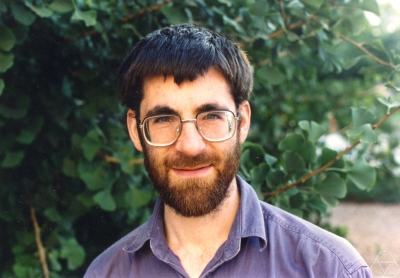
\includegraphics[scale=0.8]{images/borcherds}
\caption{Richard Borcherds.}
\end{center}
\end{figure}
\text{}
\newpage


\section{Varieties}

\subsection{Introduction}
\begin{problem}
	Classify all Pythagorean triples.
\end{problem}
We would like to solve
\begin{align*}
	x^2 + y^2 = z^2
\end{align*}
where $x$, $y$, and $z$ are integers. We shall assume that $x$, $y$, and $z$ are coprime. We know that $x^2$, $y^2$, and $z^2$ are $0$ or $1$ mod $4$, and, analyzing the equation, we see that $z$ must be odd and $x$ and $y$ must have opposite parities. Without loss of generality, we shall let $y$ be odd, and, therefore, $x$ even.

We can rearrange this as follows:
\begin{align*}
	y^2 = (z-x) (z+x).
\end{align*}
Notice that $z-x$ is prime to $z+x$. Therefore, we can write $r^2 := z-x$ and $s^2 := z+x$, so
\begin{align*}
	z &= \frac{r^2+s^2}{2};\\
	x &= \frac{s^2-r^2}{2};\\
	y&=rs.
\end{align*}
Here, $r$ and $s$ are odd and coprime.

Let us look at this problem from a geometric perspective. Again, we would like to solve
\begin{align*}
	x^2+y^2=z^2
\end{align*}
in the integers. Write $X:= x/z$ and $Y := y/z$, so
\begin{align*}
	X^2 + Y^2 =1.
\end{align*}
Now, we would like to find rational points on the unit circle. Pick a rational point $(X,Y)$ on the unit circle and draw a line between it and $(-1,0)$. Call the point at which this line intersects the $y$-axis $(0,t)$.

One sees that
\begin{align*}
	t = \frac{Y}{X+1}.
\end{align*}
Therefore, since $Y = t(X+1)$ and $X^2 + Y^2 = 1$,
\begin{align*}
	(X+1) ((t^2+1) X + t^2-1) =0.
\end{align*}
One finds that the nontrivial solution to this quadratic gives
\begin{align*}
	X &= \frac{1-t^2}{1+t^2};\\
	Y &=\frac{2t}{1+t^2}.
\end{align*}
This gives a correspondence between the points on the unit circle that are not $(-1,0)$ and points on the $y$-axis. This is called a birational equivalence\index{birational equivalence}---roughly, an equivalence except on subsets of codimension at least $1$. 

This also gives rise to the infamous Weierstrass substitution: Write $\cos \theta := X$, so $\sin \theta = Y$ and $t= \tan \theta/2$. Then, if one has an integral in $\sin \theta$ and $\cos \theta$, one can let $t = \tan\theta/2$ and use these rational expressions for $\cos\theta$ and $\sin \theta$.

Try $t=1/2$. Then $X=3/5$ and $Y=4/5$, so we find that $3^2 + 4^2 = 5^2$.

From the geometric perspective, we see that the circle forms a group (that one can identify with the group of rotations). Suppose $(x_1,y_1)$ and $(x_2,y_2)$ are points on the circle. Then, if the group operation is $\cdot$, one finds that
\begin{align*}
	(x_1,y_1) \cdot (x_2,y_2) = (x_1x_2-y_1y_2, x_1y_2+x_2y_1).
\end{align*}
Of course, this comes from the once well-known identities
\begin{align*}
	\cos(\alpha+\beta) &=\cos\alpha \cos\beta- \sin \alpha \sin \beta;\\
	\sin(\alpha + \beta) &= \sin\alpha \cos\beta + \cos \alpha \sin \beta.
\end{align*}
This is one of the simplest examples of an algebraic group\index{algebraic group}. One can think of this as a functor
\begin{align*}
	G : \catn{Ring} \longrightarrow \catn{Grp}.
\end{align*}
That is, we can take a commutative ring $R$ to the set of pairs $(x,y)\in \R^2$ such that $x^2+y^2=1$. We define the group operation as above; the identity is given by the point $(1,0)$ and $(x,y) ^{-1} = (x,-y)$.

Notice that $G(\R)$ is the unit circle. What about $G(\C)$? Well, notice that $x^2+y^2 =1$ factorizes into
\begin{align*}
	(x+iy) (x-iy) = 1.
\end{align*}
Note that $x$ and $y$ are complex. Set $z := x+iy$, and we get the pair $(z,z^{-1})$. That is, this group is the set of all nonzero complex numbers.

There are many ways to view a circle:
\begin{enumerate}
	\item A subset of $\R^2$;
	\item A polynomial $x^2 + y^2 -1$ (these first two things define an algebraic set);
	\item The ideal $(x^2+y^2-1)\subset \R[x,y]$;
	\item The ring $\R[x,y] / (x^2+y^2-1)$ (this is the coordinate ring\index{coordinate ring} of $S^1$);
	\item A (smooth) manifold;
	\item An algebraic group;
	\item A functor $\catn{Ring}\longrightarrow \catn{Grp}$ or $\catn{Ring} \longrightarrow \catn{Set}$.
\end{enumerate}

\subsection{Two cubic curves}
Consider the curve
\begin{align*}
	y^2 = x^3 + x^2.
\end{align*}
Suppose $(x,y)$ is a rational point on this curve. Draw a line between this point and $(0,0)$. The slope of this line is $y/x=t$. If we choose a line through $(0,0)$ with rational slope, it will meet the cubic curve at one other rational point. That is, $(x,y)$ being rational corresponds to $t$ being rational. This is almost a one-to-one correspondence: $(0,0)$ corresponds to $t = \pm 1$. Using the equation of the cubic, one gets that $x=t^2-1$ and $y=t^3-t$. This is another birational equivalence.

One can think of this cubic curve as a copy of the rational line except that two of the points on the rational line are identified and mapped to the same point. This is a \index{resolution of a singularity}resolution of a singularity. This resolution is done by \index{blowing up}blowing up. Hironaka proved that blowing up resolves singularities in characteristic zero.\footnote{``Resolution of singularities of an algebraic variety over a field of characteristic zero. I,'' 1964.}

\begin{example}[ ]\label{}\text{}
Find all rational points on 
\begin{align*}
	x^n+y^n = 1.
\end{align*}
Writing $x=X/Z$ and $y=Y/Z$ gives
\begin{align*}
	X^n + Y^n = Z^n.
\end{align*}
This is Fermat's last theorem, so finding rational points on curves can be hard.
\end{example}

\begin{example}[ ]\label{}\text{}
There are two glass spheres: one of radius $1$ and the other of radius $2$. Find two other glass spherees of rational radius that sum to the same value.\footnote{From \underline{The Canterbury Puzzles}, Henry Dudeney, problem 20.} That is, we want to solve
\begin{align*}
	x^3 + y^3 = 1^3 + 2^3 = 9
\end{align*}
in $\Q -\{1,2\}$. Dudeney found that
\begin{align*}
	x &= \frac{415280564497}{348671682660};\\
	y&= \frac{676702467503}{348671682660};
\end{align*}
formed another solution. How does one get this, though?

First, one draws the curve. We have two rational points on the curve already: $(1,2)$ and $(2,1)$. The tangent to $(1,2)$, for example, intersects the curve at a rational point: $(-17/7, 20/7)$. We require the coordinates be positive, though. So we draw a line between this point and $(2,1)$. The third intersection with the curve will also have rational coordinates. We determine that it is $(-271/ 438, 919/438)$. We continue this process and eventually get Dudeney's solution. 
\end{example}

This curve is not birational to a line. If a curve is birational to a line, it must be a complex sphere if one ignores some points. The curve $x^3 + y^3 =9$ looks like a torus with one point removed. Therefore, this example is fundamentally harder than the first curve and the circle.

We have an algebraic operation on this curve: Given two rational points $\alpha$ and $\beta$, we get another rational point $\alpha\cdot \beta$ by taking the third intersection of the curve and the line between $\alpha$ and $\beta$. If $\alpha$ and $\beta$ are the same point, we take the tangent to that point. Sometimes, though, we find that the line doesn't intersect with a third point. Defining a point at infinity solves this. (More on this in projective geometry.)

This operation defines a group. We let the identity be the point at infinity. We define the group law by $\alpha+\beta+\gamma = 0$ if and only if $\alpha$, $\beta$, and $\gamma$ lie on the same line. (The ``negative operation'' is what forms a group.) The operation is clearly commutative. What about associativity? It is very difficult to show that associativity holds with coordinates. However, it turns out that
\begin{align*}
	\alpha_1+\alpha_2+\cdots = \beta_1+\beta_2+\cdots
\end{align*}
if and only if there is a rational function $f$ with poles at the $\alpha_i$ and roots at the $\beta_i$. One can normally define a group structure like this on a curve.

Elliptic curves are the one-dimensional case of abelian varieties: algebraic, projective groups.
\begin{warn}
	Abelian linear groups are not abelian. ``Abelian linear group'' is an old name for ``symplectic group.'' 
\end{warn}

\subsection{B\'ezout, Pappus, Pascal}
\label{s_3}

\begin{theorem}[B\'ezout, Newton\protect\footnotemark]
	\footnotetext{\underline{Principia}, Sect. VI, Lemma XXVI.}\label{}\index{B\'ezout's theorem}\text{}
Two curves of degrees $m$ and $n$ have at most $mn$ points of intersection unless they have a common component. Two curves of degrees $m$ and $n$ in the plane have $mn$ points of intersection over $\C$ counting points at infinity and multiplicities.
\end{theorem}

Suppose the curves are given by $f(x,y)=0$ and $g(x,y)=0$ of degrees $m$ and $n$ respectively. One can assume that the number of intersection points does not change if we perturb $f$ and $g$. Write $f=p_1\cdots p_m$ and $g = q_1\cdots q_n$ as products of linear factors. Then $f$ and $g$ are a union of $m$ and $n$ lines respectively, and the result follows.

There are problems with this argument, though: How do we know that perturbing $f$ and $g$ doesn't change the number of points of intersection, for example? Proofs like this were very common in algebraic geometry before Zariski and Weil.

We shall prove this theorem later.

\begin{theorem}[Pappus]\label{}\index{Pappus's theorem}\text{}
Take two lines in the plane. Choose three collinear points and label them $1$, $2$, and $3$. Choose three more collinear points and label them $1$, $2$, and $3$. From the first line to the second, connect $1$ with $2$ and $2$ with $1$, $1$ with $3$ and $3$ with $1$, and $2$ with $3$ and $3$ with $2$. The three points of intersection are collinear.
\end{theorem}

\begin{remark}
	Pappus's theorem is equivalent to commutativity. That is, a division ring is a field if and only if Pappus's theorem holds.
\end{remark}

\begin{theorem}[Pascal]\label{}\index{Pascal's theorem}\text{}
Take an ellipse and choose six points on it. Label two points $1$, two points $2$, and two points $3$. Connect them as in the statement of Pappus's theorem. The three points of intersection are collinear. 
\end{theorem}

\begin{remark}
	Pappus's theorem is a sort of degenerate case of Pascal's theorem.
\end{remark}

\begin{proof}
Label the lines $1$ through $6$ in the order described in the statement. Choose $6$ linear polynomials $p_1,\hdots, p_{6}$ such that $p_j = 0$ on line $j$. Consider the polynomials $p_1p_3p_5$ and $p_2p_4p_6$. These vanish at all six points. The polynomial $p_1p_3p_5 - \lambda p_2p_4p_6$ also vanishes at all $6$ points. Choose $\lambda$ such that $p_1p_3p_5 - \lambda p_2p_4p_6$ vanishes at a seventh point of the conic. This polynomial has degree $3$ and the conic has degree $2$. Therefore, by B\'ezout's theorem, there are at most $2\cdot 3 = 6<7$ intersection points unless the conic and the polynomial have a common component. The conic does not split into smaller-degree polynomials, so the only way the conic and the polynomial can have a common component is if the conic is contained in the polynomial. Thus, the degree-$3$ curve is the union of a conic and a line, and this line is Pascal's line since $p_1p_3p_5$ and $p_2p_4p_6$ vanish at the points of intersection and the points are normally not on the conic. 
\end{proof}

\subsection{Kakeya sets}
A \defn{Kakeya set}\index{Kakeya set} is a set of points that contains a unit line in every direction. Examples include the radius-$1/2$ circle and the height-$1$ equilateral triangle. Kakeya conjuectured that the smallest-area Kakeya set was the three-pointed deltoid.

\begin{figure}
	\begin{center}
		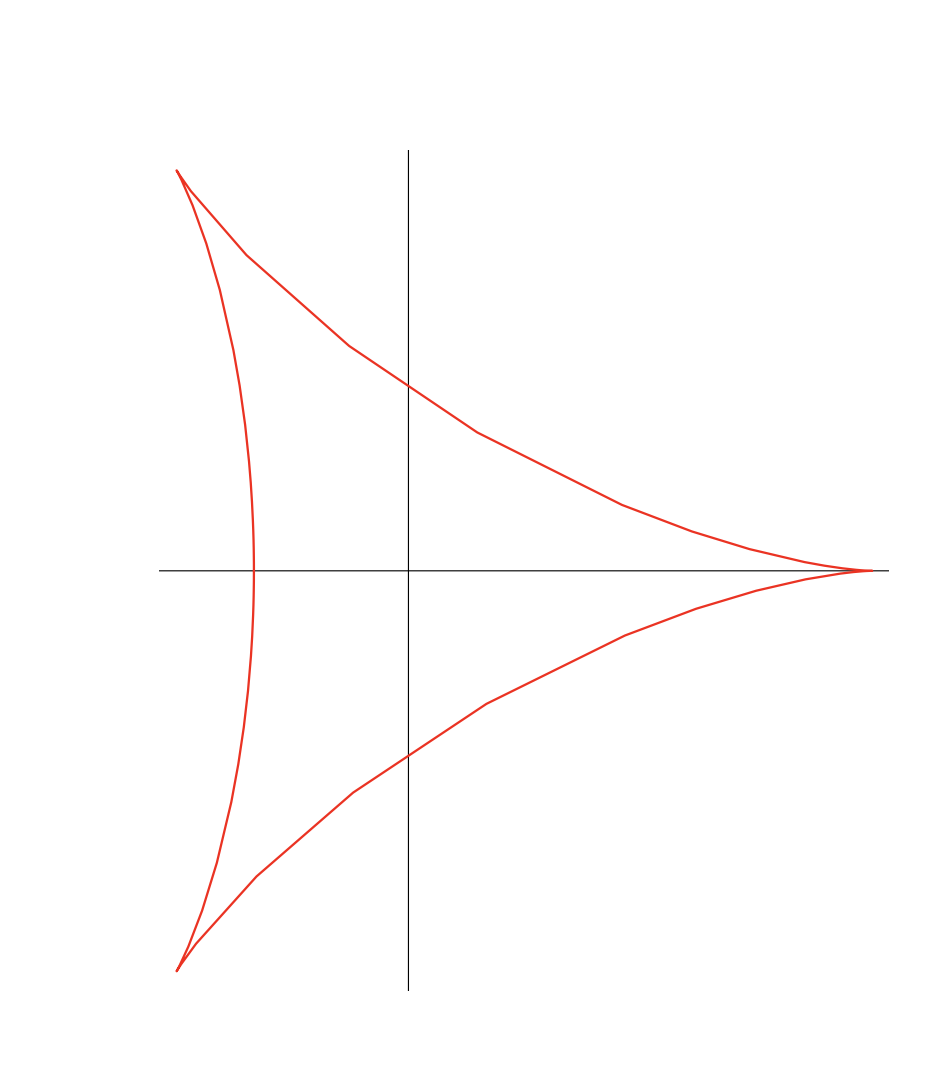
\includegraphics[scale=0.5]{images/kakeya_deltoid}
		\caption{The three-pointed deltoid.}
	\end{center}
\end{figure}

However, Besicovitch proved that there is no nonzero lower bound for the area of a Kakeya set. Thomas Wolff made the following conjecture that was proved by Dvir in 2008.\footnote{See \url{https://arxiv.org/abs/0803.2336}.}
\begin{theorem}[Wolff, Dvir]\label{}\index{}\text{}
The size of a Kakeya set over a finite field $F$ is bounded below by $c_n\left\lvert F \right\rvert ^n$.
\end{theorem}
Dvir proved this with $$c_n = \frac{1}{n!}.$$ The first step was to show that a Kakeya set cannot lie in a hypersurface of small degree. The second step was to show that, if a set is small, one can find a hypersurface of small degree containing it.

First, we claim that a Kakeya set in $F^n$ cannot lie in a hypersurface of degree $d<\left\lvert F \right\rvert $. Suppose $f$ is a polynomial of degree $d<\left\lvert F \right\rvert $ defining a hypersurface. Let $f_d$ be the highest-degree component. For any $v$, one can find $x$ such that $f(x+vt)$ vanishes for all $t$. This means that the roots of $f$ form a Kakeya set. Therefore, the coefficient $f_d(v)$ of $t^d$ vanishes. This is true for all $v$ and $f_d$ has degree less than $\left\lvert F \right\rvert $, so $f_d=0$. Thus, $f=0$.

Observe that the polynomials of degree less than or equal to $\left\lvert F \right\rvert -1$ form a vector space of dimension $\binom{n+\left\lvert F \right\rvert -1}{n}$. Therefore, one can find a hypersurface of degree at most $\left\lvert F \right\rvert -1$ vanishing on any set with less than $\binom{n+\left\lvert F \right\rvert -1}{n}$ points.

Thus, one concludes that Kakeya sets have at least $\binom{n+\left\lvert F \right\rvert -1}{n}$ points. This quantity is 
\begin{align*}
	\binom{n+\left\lvert F \right\rvert -1}{n} &= \frac{(\left\lvert F \right\rvert ) \cdots (\left\lvert F \right\rvert +n-1)}{n!} \\
						   &\ge \frac{\left\lvert F \right\rvert ^n}{n!}
\end{align*}
as required.

The following example is sometimes said to be the beginning of higher-dimensional algebraic geometry.

\begin{example}[$27$ lines on a cubic surface]\label{}\text{}
Cayley and Salmon proved that any nonsingular cubic surface has exactly $27$ lines on it. Consider the surface
\begin{align*}
	w^3 + x^3 +y^3 + z^3 = 0 \subset \mathbf{P}^3.
\end{align*}
(Projective space is the set of quadruples $(w,x,y,z)$ modulo the equivalence relation $(w,x,y,z)\sim  (\lambda w, \lambda x, \lambda y,\lambda z)$ for $\lambda\ne 0$. That is, if $z\ne 0$, one can take $\{(w,x,y,1)\} \isomto  \mathbf{C}^3$. One can see that $\mathbf{P}^3$ is covered by four copies of affine space.) The line $(a,-a,b,-b)$ is on this surface. We can permute the coordinates and multiply by a cube root of unity. This gives $3^3 = 27$ lines.  
\end{example}

\subsection{Affine space and the Zariski topology}
Let $K$ be a field. Then \index{affine space}affine space is almost the vector space $K^n$. The automorphisms of this vector space are all invertible linear transformations, given by $\GL_{n}(K)$. The automorphisms of affine space which one denotes $\A^n(K)$ include $\GL_{n}(K)$ and translations $x \longmapsto x+v$. Therefore, the group of automorphisms of affine space is of dimension $n(n+1)$ and consists of matrices of the form
\begin{align*}
	\mat{*&*&*\\ \text{}*&*&*\\0&0&1}
\end{align*}
where the $2\times 2$ matrix in the top left has nonzero determinant. Roughly speaking, a vector space has an origin and an affine space does not. That is, one has a forgetful functor from vector spaces to affine spaces that forgets about the origin. One goes the other way by choosing an arbitrary origin. 

\iffalse Consider the three-dimensional pre-Einstein space in which we live. This is affine space blakdnkjdn Wait it has a metric\fi

\index{affine geometry}Affine geometry can be thought of as the study of the properties of affine space invariant under affine symmetries: invariant under translations and linear transformations. \iffalse Let us list some well-defined things in affine geometry:
\begin{itemize}
	\item Points;
	\item Lines;
	\item Parallel lines;
	\item Conics;
	\item Polynomial functions.
\end{itemize}
The following things are not well-defined.
\begin{itemize}
	\item Circles;
	\item Angles;
	\item Lengths.
\end{itemize}\fi Points, lines, parallel lines, conics, and polynomial functions are well defined in affine geometry. One realizes that circles, angle, and lengths, for example, are not well defined.

Algebraic geometry tends to use the \index{coordinate ring}coordinate ring of $\mathbf{A}^n(K)$; that is, polynomials on the affine space: $K[x_1,\hdots, x_n]$. Given a coordinate ring, one can get an affine space $\A^n(K)$ by taking the set of all $K$-algebra homomorphisms from the polynomial ring to $K$. The automorphism groups of these two things are the same, for example.

\begin{definition}[Algebraic set]\label{}\text{}
An \defn{algebraic set}\index{algebraic set} in $\mathbf{A}^n(K)$ is the set of common roots of a set of polynomials in $K[x_1,\hdots, x_n]$.
\end{definition}

\begin{example}[ ]\label{}\text{}
Suppose $f=x^2+y^2-1$. Then the algebraic set is a circle. Suppose we have $\{x-\alpha,y-\beta\}$. Then the algebraic set is $\{(\alpha,\beta)\}$.
\end{example}

Algebraic sets are closed under intersections. If $C_1,C_2,\hdots $ are the set of roots of $P_1,P_2,\hdots$ respectively, then $C_1\cap C_2\cap \cdots $ is the set of roots of $P_1\cup P_2\cup \cdots$. They are also closed under finite unions. If $C_1$ and $C_2$ are the sets of roots of $\{f_1,f_2,\hdots\}$ and $\{g_1,g_2,\hdots\}$, then $C_1\cup C_2$ is the set of roots of $\{f_ig_j\}$.

If a collection of sets is closed under intersections and finite unions, they form the closed sets of a topology. Therefore, \index{algebraic set}algebraic sets are the closed sets of the Zariski topology. (The intersections do not need to be of countably many sets.)

What are the closed sets of the affine line $\mathbf{A}^1(K)$? The line is the set of roots of $0$. Any finite set consists of the roots of a polynomial $(x-\alpha_1)(x-\alpha_2)\cdots(x-\alpha_n)$. One can check that $\mathbf{A}^1(K)$ and finite sets are the only closed sets. One notes that this topology is not Hausdorff.

What about $\mathbf{A}^2(K)$? We have sets of points $\{(\alpha,\beta)\}$ that is the set of common roots of $\{x-\alpha, y-\beta\}$. We also have any algebraic curve $f(x,y) =0$. Therefore, a typical closed set in $\mathbf{A}^2(K)$ consists of finitely many algebraic curves and points. One notices that the Zariski topology on $\mathbf{A}^2(K)$ is not the product topology on $\mathbf{A}^1(K)\times \mathbf{A}^1(K)$. The latter is a finite number of vertical lines, horizontal lines, and points.

\begin{example}[Determinantal variety]\label{}\text{}
One can think of $\mathbf{A}^{mn}(K)$ as the vector space of linear maps $K^m \longrightarrow K^n$ or of $m\times n$ matrices of dimension $mn$. An algebraic set is given by all linear maps of rank at most $r$ for some $r$. This gives the \index{determinantal variety}determinantal variety. This set is given by the vanishing of all $(r+1)\times  (r+1)$ minors of an $m\times n $ matrix. For example, the subset of surjective maps $K^m\longrightarrow K^n$ is open in the Zariski topology.
\end{example}

\subsection{Noetherian spaces}
\begin{definition}[ ]\label{}\text{}
A \defn{Noetherian ring}\index{Noetherian ring} $R$ satisfies one of these three equivalent conditions:
\begin{enumerate}
	\item Every ideal of $R$ is finitely generated;
	\item Every nonempty set of ideals has a maximal element;
	\item Every increasing chain of ideals stabilizes. 
\end{enumerate}
\end{definition}

\begin{example}[ ]\label{}\text{}
The ring $K[x_1,\hdots, x_n]$ is Noetherian. Hilbert originally proved this. Noether gave a much simpler proof as follows. She showed that if $R$ is Noetherian, then $R[x]$ is Noetherian. Consider $I_0\subseteq I_1\subseteq\cdots$ of $R$ where $I_n$ is given by the leading coefficients of polynomials of degree less than or equal to $n$ in an ideal $I\subseteq R$. We know that $I_N=I_{N+1}=\cdots$ for some $N$ since $R$ is Noetherian. Take finite sets of polynomials $S_0,S_1,\hdots, S_N$ where $S_k$ contains polynomials of degree $k$ whose leading coefficients generate $I_k$. One can check $S_0,\hdots, S_N$ generate $I$. 
\end{example}

\begin{definition}[ ]\label{}\text{}
A topological space is a \defn{Noetherian topological space}\index{Noetherian topological space} if, equivalently,
\begin{enumerate}
	\item The closed sets satisfy the descending chain condition, so any decreasing chain of closed sets stabilizes;
	\item Any nonempty collection of closed sets has a minimal element.
\end{enumerate}
\end{definition}
 \begin{remark}
 	The affine space $\mathbf{A}^n(K)$ with the Zariski topology is Noetherian. Closed sets of $\mathbf{A}^n(K)$ correspond to some ideals of the coordinate ring $K[x_1,\hdots, x_n]$. (Any closed set is determined by the ideal of functions vanishing on it.)
 \end{remark}

Noetherian spaces are weird. The Noetherian condition is equivalent to saying that every open set is (quasi)compact. (Bourbaki changed the definition of ``compact'' to mean compact and Hausdorff, but it turned out that there were non-Hausdorff compact sets, so they used the term ``quasicompact.''\index{compact}\index{quasicompact}\footnote{See \underline{General Topology}, \S 9.I, p. 83.}) 

\begin{exercise}\label{}\text{}
Show that if a topological space is Noetherian and Hausdorff then it is finite.
\end{exercise}

\begin{definition}[ ]\label{}\text{}
A topological space is called an \defn{irreducible topological space}\index{irreducible topological space} if it is nonempty and not the union of two proper closed subsets.
\end{definition}

Recall that a typical closed set of $\mathbf{A}^2(K)$ is a finite number of curves and points. The curves are irreducible. An affine line, for example, is irreducible since any two nonempty closed sets intersect. This space seems to be the union of a finite number of irreducible subsets.

\begin{theorem}[ ]\label{}\index{}\text{}
Any Noetherian space is a finite union of irreducible subspaces.
\end{theorem}

\begin{proof}
This follows from Noetherian induction. Every closed subset is a finite union of irreducibles. If not, pick a minimal counterexample $C$. If $C$ is irreducible, then we are done, since we have a contradiction. If $C$ is not irreducible, then we can write $C=C_1\cup C_2$ where $C_1$ and $C_2$ are smaller closed subsets. By induction, $C_1$ and $C_2$ are finite unions of irreducibles and, therefore, $C$ is. This is a contradiction. 
\end{proof}

\begin{corollary}[ ]\label{}\text{}
Every algebraic set is a finite union of irreducible algebraic sets.
\end{corollary}

\begin{remark}
	Irreducible algebraic sets are sort of (provisionally) \index{algebraic variety}algebraic varieties.
\end{remark}

\begin{example}[ ]\label{}\text{}
Consider the variety $xy=1$ and the set of nonzero points in $\mathbf{A}^1$. The temporary definition of an algebraic variety means that the set of nonzero points is not an algebraic variety. However, one sees that these two objects are isomorphic. We shall address this later.
\end{example}

\begin{example}[ ]\label{}\text{}
Consider the algebraic set $\{x^2+y^2 -2z^2=0, 2x^2 - y^2 - z^2=0\}$. This turns out to be a union of four irreducible subsets (lines): $x=y=z$, $x=-y=z$, $x=-y=-z$, and $x=y=-z$. The intersection of irreducible subsets does not need to be irreducible.
\end{example}

\begin{example}[ ]\label{}\text{}
Take $xy=0$. This is reducible but connected. Now, consider $xy=1$. This is irreducible, and it certainly doesn't look connected. However, it is connected in the Zariski topology (of course, it isn't in the Euclidean topology).
\end{example}


\subsection{Weak Nullstellensatz}
Let us study the relationship between subsets of an affine space $\mathbf{A}^n$ and ideals of $K[x_1,\hdots, x_n]$. One can map a subset $Y$ to the ideal $\II(Y)$ given by polynomials vanishing on $Y$. Conversely, an ideal $\mathfrak{a}$ can be mapped to a subset $\ZZ(\mathfrak a)$ given by the set of roots of $\mathfrak{a}$. What is the relationship between these two maps? Well, $\ZZ(\II(Y))$ is the closure of $Y$ in the Zariski topology. Further, $\II(\ZZ(\mathfrak{a}))\ne \mathfrak{a}$. For example, take $\mathfrak{a}=(x^2)\subset K[x]$. Then $\ZZ(\mathfrak{a}) = \{0\}$, so $\II(\ZZ(\mathfrak{a})) =(x)\ne (x^2)$. More generally, if $f^n\in \mathfrak{a}$, then $f\in \II(\ZZ(\mathfrak a))$. So $\sqrt{\mathfrak{a}} \subseteq \II(\ZZ(\mathfrak{a}))$. Recall that\index{radical of an ideal}
\begin{align*}
	\sqrt{\mathfrak{a}} := \{ r\in R : r^n \in \mathfrak{a} \textrm{ for some $n$}\}.
\end{align*}
Also recall that the radical is an ideal.

\begin{problem}
	Does $\sqrt{\mathfrak{a}}= \II(\ZZ(\mathfrak{a})) $ hold?
\end{problem}

No. Take $\mathfrak{a} = (x^2 + 1) \subset \R[x]$. Notice that $\ZZ(\mathfrak{a})= \emptyset$, so $\II(\ZZ(\mathfrak{a})) = \mathbf{R}[x]\ne \mathfrak{a}$. (This has to do with $\mathbf{R}$ not being algebraically closed.) However, if $\Omega$ is algebraically closed, then the equality holds. (This will be Hilbert's \index{Nullstellensatz}Nullstellensatz.) 

\begin{problem}
	What are the maximal ideals of $K[x_1,\hdots, x_n]$?
\end{problem}

There are some obvious ones. Take $(a_1,\hdots, a_n)\in \mathbf{A}^n$. Consider the ideal $(x_1-a_1,\hdots, x_n-a_n)$. This consists of the functions vanishing on $(a_1,\hdots, a_n)$. It is maximal because its quotient by the ring is $K$. Are these all maximal ideals? No. But it is true if $K$ is algebraically closed. This is the \index{weak Nullstellensatz}weak Nullstellensatz  (as opposed to the \index{strong Nullstellensatz}strong Nullstellensatz above). Let us prove this.

First, we shall show that if $K$ is a field and finitely generated as an algebra over $k$, then $K$ is a finitely generated module over $k$. We're going to cheat by assuming that $k$ is uncountable. Notice that $K$ is of at most countable dimension as a module since it is finitely generated as an algebra. If $x\in K$ is transcendental over $k$, then the elements $1/(x-a)$ for $a\in k$ form an uncountable, linearly independent set. This is a contradiction. Therefore, all $x\in K$ are algebraic over $k$. Since $K$ is finitely generated as an algebra, $K$ is finitely generated as a module (or vector space). (One does not require $k$ to be uncountable: The finite number of generators of $K$ only have poles on a finite number of irreducible subsets of the affine space over $k$, but there are an infinite number of such irreducible subsets.)

Suppose $I$ is a maximal ideal of $k[x_1,\hdots, x_n]$. We want to show that $I = (x_1-a_1,\hdots, x_n-a_n)$ for some $(a_1,\hdots, a_n)$. Put $K = k[x_1,\hdots, x_n]/I$, which is a field since $I$ is maximal. The field $K$ is also finitely generated by an algebra (generated by $x_1,\hdots, x_n$). By  the previous ``lemma,'' $K$ is finitely generated as a module; that is, $K$ is algebraic over $k$. But $k$ is algebraically closed, so $k=K$. Therefore, each $x_i\in K$, so $x_i=a_i$ for some $a_i\in k$. This implies that $I\supseteq (x_1-a_1,\hdots, x_n-a_n)$. So $I = (x_1-a_1,\hdots, x_n-a_n)$. The weak Nullstellensatz follows.


\subsection{Strong Nullstellensatz}
Suppose $K$ is an algebraically closed field. Recall the weak and strong Nullstellensatz.\index{Nullstellensatz}\index{weak Nullstellensatz}\index{strong Nullstellensatz}

\begin{theorem}[Weak Nullstellensatz]\label{}\index{}\text{}
The maximal ideals of $K[x_1,\hdots, x_n]$ correspond to points in affine space.
\end{theorem}

\begin{theorem}[Strong Nullstellensatz]\label{}\index{}\text{}
Suppose $\mathfrak{a}\subseteq K[x_1,\hdots, x_n]$ is an ideal. Then 
\begin{align*}
	\II(\ZZ(\mathfrak{a})) = \sqrt{\mathfrak{a}} .
\end{align*}
\end{theorem}

\begin{proof}
It is straightforward to show that $\sqrt{\mathfrak{a}} \subseteq \II(\ZZ(\mathfrak{a}))$. We shall employ the Rabinowitsch trick.\footnote{See ``Zum Hilbertschen Nullstellensatz,'' 1929.} Suppose $\mathfrak{a}$ is generated by $f_1,\hdots, f_m$ and $f\in \II(\ZZ(\mathfrak{a}))$. We want to show $f\in \II(\ZZ(\mathfrak{a}))$. This means that $f$ vanishes if $f_1,\hdots, f_m$ vanish. Therefore, $f_1,\hdots, f_m$ and $1-x_0f$ have no common roots in $\mathbf{A}^{n+1}$ (bringing in another variable is the trick of Rabinowitsch). Apply the weak Nullstellensatz to $\mathbf{A}^{n+1}$. Therefore, $f_1,\hdots, f_m, 1-x_0f$ generate the unit ideal. That is, $(f_1,\hdots,f_m,1-x_0f) = (1) = K[x_0,\hdots, x_n]$, hence $1 = g_0(1-x_0f)+g_1f_1 +\cdots + g_mf_m$ for some $g_i$. Put $x_0=1/f$, so $1=g_1f_1+\cdots +g_mf_m$ where $g_i \in K[x_1,\hdots, x_n, 1/f]$. Clearing denominators, one has
\begin{align*}
	f^N = h_1f_1+\cdots + h_mf_m
\end{align*}
where $h_i=g_if^N\in K[x_1,\hdots, x_n]$. That is, $f\in \sqrt{(f_1,\hdots, f_m)} $.
\end{proof}

Hilbert's Nullstellensatz gives a correspondence between affine space $\mathbf{A}^n$ and the ring $K[x_1,\hdots, x_n]$. Points correspond to maximal ideals. Algebraic sets correspond to radical ideals $\mathfrak{a} = \sqrt{\mathfrak{a}} $. More generally, closed subschemes correspond to ideals.

\begin{example}[ ]\label{}\text{}
Consider the line $y=0$ that corresponds to the ideal $(y)$ and the parabola $y=x^2$ that corresponds to the ideal $(y-x^2)$. These are radical ideals. One takes the intersection of these two varieties by taking $(y-x^2, y)$. This ideal is not radical, since $\sqrt{(y, x^2)}=(x,y)$ as an ideal which corresponds to $(0,0)$ as a point in affine space.
\end{example}


\begin{example}[Nilpotent matrices]\label{}\text{}
Recall that $A\in \MM_n(K)$ is nilpotent if $A^n = 0$. One can think of $\MM_n(K)$ as $\mathbf{A}^{n^2}$. If $A = (a_{ij})$, then $A^n$ is something complicated, but suppose its entries generate the ideal $I$ in the coordinate ring of $\mathbf{A}^{n^2}$. Does $I=\sqrt{I} $ hold? No. If $A$ is nilpotent, then all of its eigenvalues are $0$, so its trace is $0$. But $\sum_{j}^{} a_{jj}\notin I$ since $I$ is generated by homogeneous polynomials of degree $n$ and $\sum_{j}^{} a_{jj} \in \sqrt{I} $ by the Nullstellensatz.

Take $n=2$. If 
\begin{align*}
	A = \mat{a&b\\c&d}
\end{align*}
is nilpotent, then
\begin{align*}
	A^2 = \mat{a^2 + bc&b(a+d)\\c (a+d) &d^2 + bc} = 0.
\end{align*}
Hence $I=   (a^2+bc,\, b(a+d), \,c (a+d),\,d^2 + bc)$. Some power of $a+d$ is an element of $I$. What is the smallest such power? Exercise: Show that $(a+d)^2\notin I$ but $(a+d)^3\in I$.
\end{example}

\begin{example}[Commuting matrices]\label{}\text{}
Write $A=(a_{ij})$ and $B=(b_{ij})$. Then $AB-BA$ is something; let its entries generate the ideal $I$ in the coordinate ring of $\mathbf{A}^{2n^2}$. Whether or not $I=\sqrt{I} $ holds is an open problem. The question of whether an ideal $I\subset R$ is radical is the same as asking whether $R/I$ has nilpotent elements. (The space of pairs of commuting matrices is a notoriously difficult space to study.)
\end{example}

\subsection{The Lasker--Noether theorem}
Recall that algebraic sets correspond to radical ideals of $K[x_1,\hdots, x_n]$. Also, an algebraic set is a finite union of irreducible algebraic sets. Irreducible algebraic sets correspond to prime ideals. (Recall that an ideal $\mathfrak{p}\subseteq R$ is prime if $R/\mathfrak{p}$ is an integral domain.)

\begin{theorem}[ ]\label{}\index{}\text{}
A radical ideal is a finite intersection of prime ideals.
\end{theorem}

This is a translation of the previously-mentioned result into ring-theoretic language.
\begin{theorem}[Lasker]\label{}\index{}\text{}
An ideal of $K[x_1,\hdots, x_n]$ is a finite intersection of primary ideals.
\end{theorem}
\begin{theorem}[Noether]\label{}\index{}\text{}
This holds for ideals of Noetherian rings.
\end{theorem}\index{Lasker--Noether theorem}
\iffalse
\begin{remark}
	Emmanuel Lasker was World Chess Champion for 27 years, which is the longest anyone has held this title. He proved the theorem above during his reign.
\end{remark}
\fi

\begin{definition}\label{}\text{}
An ideal $\mathfrak{p}\subseteq R$ is \defn{primary}\index{primary ideal} if and only if $ab\in \mathfrak{p}$ implies $a\in \mathfrak{p}$ or $b^n\in \mathfrak{p}$ for some $n$.
\end{definition}

Alternatively, suppose if $ab=0$ where $a\in R$ and $b\in R/\mathfrak{p}$ then $b=0$ or $a^n=0$ for some $n$. Then $R/\mathfrak{p}$ is \defn{coprimary}\index{coprimary module}. The module $R/\mathfrak{p}$ is coprimary if and only if $\mathfrak{p}$ is primary.

\begin{definition}[ ]\label{}\text{}
A module $M$ is coprimary if it has at most one associated prime.
\end{definition}

\begin{definition}[ ]\label{}\text{}
An \defn{associated prime}\index{associated prime} $\mathfrak{p}$ of a module $M$ over $R$ is a prime ideal such that $M$ contains a submodule isomorphic to $R/\mathfrak{p}$.
\end{definition}
\begin{remark}
If $R$ is Noetherian, these two definitions of coprimary are equivalent for finitely generated modules.
\end{remark}

If one has modules $M\supseteq N$, $N$ is primary if and only if $M/N$ is coprimary.

\begin{theorem}[Lasker--Noether]\label{}\index{}\text{}
Let $M$ be a finitely generated module over a Noetherian ring $R$. The ideal $(0)$ is an intersection of primary submodules of $M$. Equivalently, $M$ is contained in a finite direct sum of coprimary modules.
\end{theorem}

For $\mathbf{Z}$-modules, coprimary modules include $\mathbf{Z}^n$ where $\mathfrak{p}=(0)$ and any finite group of order $p^f$ where $\mathfrak{p} = (p)$. Recall that abelian groups are a direct sum of free abelian groups and groups of prime power order.

\subsection{The Lasker--Noether theorem}
The video in which Dr. Borcherds proves the Lasker--Noether theorem is incomprehensible, so this section comes from a video from his series on commutative algebra.\footnote{The link: \url{https://www.youtube.com/watch?v=GLmXzrusM2M}.}

Let $M$ be a finitely generated module over a Noetherian ring $R$. Recall that $M$ is coprimary if it has at most one associated prime. We shall prove that
\begin{align*}
	M \subseteq \bigoplus_{\mathfrak{p}\in \Ass M} M_{\mathfrak{p}}
\end{align*}
where each $M_{\mathfrak{p}}$ is coprimary with associated prime $ \mathfrak{p}$. 

There is no such thing as a primary module. The original version of the theorem says that if $I\subseteq R$ is an ideal, then $I$ is a finite intersection of primary ideals. Lasker originally proved this for polynomial rings over fields $K$ or $\mathbf{Z}$. His proof was incredibly long. Noether generalized the result to all Noetherian rings. Her proof was notably simpler.

The second version is as follows. Suppose we have modules $N\subseteq M$. Then $N$ is a finite intersection of primary submodules.

\begin{definition}[ ]\label{}\text{}
A submodule $X$ is called a \defn{primary submodule}\index{primary submodule} of $M$ if $rm\in X$ implies $m\in X$ or $r^nM\subseteq X$ for some $n>0$.
\end{definition}

Notice that if $M=R$, then a submodule is an ideal, and this becomes Lasker's definition of a primary ideal. One notes that this is not a property of $X$; it is a property of how $X$ is embedded in $M$. In particular, it is a property of the quotient $Y:= M/X$. If $r$ is a zero divisor of $Y$, then $r^nY=0$ for some $n>0$. The module $Y$ with this property is coprimary. We will show that this definition and the one mentioned earlier are equivalent for finitely generated modules.

The third version of the Lasker--Noether theorem says that
\begin{align*}
	M \subseteq \prod_{\mathfrak{p}\in \Ass M} M_{\mathfrak{p}}
\end{align*}
where $M_{\mathfrak{p}}$ is coprimary. In fact, the second version implies this one. 

Take $N=0$, so $0 = \bigcap J_{\mathfrak{p} }$ where $J_{\mathfrak{p}}$ is a primary submodule. That is, the natural map $M \longrightarrow \prod M/J_{\mathfrak{p}}$ is injective (the kernel is the intersection that is $0$). Although $J_{\mathfrak{p}}$ is a primary submodule, the quotient is coprimary.

We have two definitions for ``coprimary'':
\begin{enumerate}
	\item There is at most one associated prime;
	\item $rm = 0$ implies $m=0$ or $r^nM=0$ for some $n>0$.
\end{enumerate}

Suppose $n\ne 0$ and $m\in M$. Put $\mathfrak{p} = \Ann(m)$. Then the second definition implies $\mathfrak{p} \subseteq \sqrt{\Ann (M)} $. If $\mathfrak{p}$ is prime, then $\Ann(M)\subseteq \Ann (m)= \mathfrak{p}$, so $\sqrt{\Ann(M)}\subseteq \mathfrak{p} $. That is, if $\mathfrak{p}\in \Ass M$, $\mathfrak{p} = \sqrt{\Ann (M)} $. Thus, there is at most $1$ associated prime given by the radical of the annihilator of $M$. So 2. implies 1.

Assume $\Ann M=0$. Put $\Ass M = \{\mathfrak{p}\}$. This associated prime contains $\Ann (m)$ given $m\ne 0$. Therefore, we need to show that $\mathfrak{p}$ is nilpotent. Suppose $a\in \mathfrak{p}$ is nilpotent. Then the localization $M[a^{-1}]$ is nonzero. If $x\in M$ is $0$ in $M[a^{-1}]$ , then $xa^n=0$ for some $n$. That is, $M[a^{-1}]=0$ implies $a^n \in \Ann M$ for some $n$ since some power kills any element of $M$ and $M$ is finitely generated. But $\Ann M=0$ by assumption, so $a$ is nilpotent. 

Since $M[a^{-1}]\ne 0$, one has $\Ass (M[a^{-1}])\ne \emptyset$ (primes of $R[a^{-1}]$). Pick $T\in \Ass (M[a^{-1}])$, an ideal of $R[a^{-1}]$. Let $\mathfrak{q}$ be the preimage of $T$ in $R$. (Recall we have $R\longrightarrow  R[a^{-1}]$, $\mathfrak{q}\longrightarrow T$, $\mathfrak{q}\subseteq R$, and $T\subseteq R[a^{-1}]$.) Both $T$ and $\mathfrak{q}$ are primes, and $\mathfrak{q}$ is the union of $\Ann(m)\subseteq \Ann (ma)\subseteq \Ann (ma^2)\subseteq \cdots$. (One verifies that $\mathfrak{q}$ is everything that annihilates $ma^n$.) This is an increasing sequence in a Noetherian ring, so it stabilizes. Therefore, $\mathfrak{q}=\Ann(ma^n)$ for some $n$. Hence, $\mathfrak{q}\in \Ass(M)$ since it is prime and the annihilator of some element in $M$. But $a\in \mathfrak{p}$ and $a\notin \mathfrak{q}$ because $a$ is a unit of $M[a^{-1}]$ and if $a\in \mathfrak{q}$ then $M[a^{-1}]=0$. So $\mathfrak{p}\ne \mathfrak{q}$, so $M$ has at least $2$ associated primes. Contradiction. So 1. implies 2.

Now, we prove the Lasker--Noether theorem that 
\begin{align*}
	M\subseteq \prod_{\mathfrak{p} \in \Ass M} M_{\mathfrak{p}}
\end{align*}
where $M_{\mathfrak{p}}$ is coprimary.  

If it is not true, pick a maximal submodule $N$ such that $M/N$ is not contained in a product of coprimary ideals. We may assume that $N=0$ by modding out by $N$. Notice that $M$ is not coprimary, so it has $2$ submodules $M_1\isomto R/\mathfrak{p}_1$ and $M_2\isomto R/\mathfrak{p}_2$ where $\mathfrak{p}_1\ne \mathfrak{p}_2$ are primes. Then, for $x\in R/\mathfrak{p}_1- \{0\}$, $\Ann(x)= \mathfrak{p}_1$, and similarly for $\mathfrak{p}_2$. Therefore, $M_1\cap M_2=0$. Consider this exact sequence:
\begin{align*}
	M_1\cap M_2 \longrightarrow M\longrightarrow M/M_1 \oplus M/M_2.
\end{align*}
Since the intersection is zero, the second arrow is injective. Moreover, we assumed that $0$ is the maximal submodule not a product of coprimary modules, so each quotient is contained in a product of coprimary modules. Therefore, $M$ is contained in a product of coprimary modules. The Lasker--Noether theorem follows.

Take $M=R/I$. We have 
\begin{align*}
	R/I = M \subseteq \prod_{} R/I_{\mathfrak{p}}.
\end{align*}
We know that the $R/I_{\mathfrak{p}}$, so $I_\mathfrak{p}$ must be primary in Lasker's sense. Therefore, $I=\bigcap I_\mathfrak{p}$.

\subsection{Quotients of varieties by groups}
Recall that any algebraic set $Y$ has a coordinate ring $K[x_1,\hdots, x_n]/\II(Y)$. This coordinate ring is an algebra over $K$, is finitely generated, and has no nilpotent elements. Further, a ring with these three properties corresponds to an algebraic set by the Nullstellensatz. (This algebraic set is not unique; it depends on the choice of generators. The corresponding algebraic sets are isomorphic in a sense.) One can think of algebraic sets up to some kind of isomorphism as being equivalent to rings with these three properties. The category of algebraic sets is equivalent to the opposite category of coordinate rings. 

Suppose $Y$ is an algebraic set acted on by a group $G$. Can we form a quotient $Y/G$? One cannot form a quotient by identifying points of $Y$ with elements of $G$. One views this problem from the perspective of coordinate rings. 

If the group $G$ acts on the algebraic set $Y$, it will act on the corresponding coordinate ring. Therefore, we look at the ring of invariants $(K[x_1,\hdots,x_n]/\II(Y))^G$. If the invariant ring satisfies the three previous properties, then it is the coordinate ring of an algebraic set, so it is reasonable to call it $Y/G$.

This invariant ring is clearly a $K$-algebra. It has no nilpotent elements, either. But is it finitely generated? Hilbert proved that it is in many cases, but Nagata proved that that's not always the case.\footnote{``On the fourteenth problem of Hilbert,'' 1958, \url{https://web.archive.org/web/20131102202816/http://www.mathunion.org/ICM/ICM1958/Main/icm1958.0459.0462.ocr.pdf}.}

\begin{example}[ ]\label{}\text{}
Suppose $G=\Sg_n$ acts on $\mathbf{A}^n$ by permuting coordinates. Then $K[x_1,\hdots, x_n]^G$ is the ring of invariant functions generated by the elementary invariant polynomials. Hence, one sees that $\mathbf{A}^n/\Sg_n\isomto \mathbf{A}^n$. (This works out so nicely because $\Sg_n$ is a reflection group.)
\end{example}


If $\Zmod 2$ acts on the real line by $x\longmapsto -x$, one might think that the quotient is a half-closed interval. This is what one gets by identifying points under the group, but, by the construction above, it's the real line. One identifies $2$ and $-2$, but also identifies $2i$ and $-2i$ (these are real points of the quotient).


 \begin{example}[ ]\label{}\text{}
Suppose $\GL_{n}(K)$ acts on $K^n$. The orbits are either $0$ or everything else, so one is led to believe that the quotient will have two points. However, it only has one, since the only invariant polynomials acted on by $\GL_{n}(K)$ are constants. That is, we get the field $K$: the coordinate ring of a point.
\end{example}

\begin{example}[Classical invariant theory]\label{}\text{}
The group $G=\SL_{2}(\mathbf{C})$ acts on binary quantics (binary forms) $a_nx^n + a_{n-1}x^{n-1}y + \cdots +a_0y^n$. We have $(a_0,\hdots, a_n)\in \mathbf{A}^{n+1}$. What is the quotient $\mathbf{A}^{n+1}/\SL_{2}(\mathbf{C})$? The coordinate ring of this will be all polynomials in $a_n,a_{n-1},\hdots$ invariant under $\SL_{2}(\mathbf{C})$. These are called \index{invariants}invariants. 

Take $a_2x^2 + a_1xy + a_0y^2$. A typical invariant is the discriminant, given by $a_1^2 - 4a_0a_2$. Paul Gordan proved that the ring of invariants was finitely generated.\footnote{See \underline{Mathematics of the 19th Century: Mathematical Logic, Algebra, Number Theory, Probability Theory}, 2001, p. 85.} Gordan was known as the ``king of invariant theory.'' His proof was convoluted, but Hilbert figured out a way to prove that rings of invariants were finitely generated. We shall look at this in the next section.
\end{example}

\subsection{Hilbert's finiteness theorem}
Let $A$ be the ring $K[x_1,\hdots, x_n]$. Let $G$ be a group acting on $K^n$ spanned by $x_1,\hdots, x_n$. That is, the group $G$ acts on $A$. We consider $A^G$: the invariant elements of $A$ under the action of $G$. Is $A^G$ finitely generated as a $K$-algebra?

\begin{theorem}[Hilbert]\label{}\index{Hilbert's finiteness theorem}\text{}
The invariant ring $A^G$ is finitely generated as a $K$-algebra if $G$ is finite and $\chr K = 0$.
\end{theorem}
\begin{remark}
	Hilbert proved this for almost any reductive group. The restriction on the characteristic of $K$ is not necessary, but it simplifies the proof.
\end{remark}

Notice that $A$ is graded by degree, so $A = A_0\oplus A_1\oplus A_2\oplus \cdots$. Let $I$ be the ideal of $A$ generated by the homogeneous elements of $A^G$ of degree greater than $0$. Notice that $I$ is finitely generated as an ideal. We can assume that $I$ has a finite number of generators in $A^G$, and they are homogeneous. 

Suppose $I=(i_1,\hdots,i_n)$ as above. We would like to show that these elements generate $A^G$ as a $K$-algebra. Suppose $A=K[x,y]$ and $I = (y)$. Even though $I$ is finitely generated as an ideal, the ring it gives is not finitely generated as a ring or algebra (it is generated by $y, xy, x^2y,\hdots$). 

The ring of invariants $A^G$ of $A$ has a Reynolds operator\index{Reynolds operator} $\rho$. The Reynolds operator $\rho(a)$ of $a$ is the average of $a$ under $G$, so
\begin{align*}
	\rho(a) = \frac{1}{\left\lvert G \right\rvert } \sum_{g\in G}^{} g(a).
\end{align*}
(Notice that we needed that $G$ is finite and $\chr K = 0$.) It has the following properties:
\begin{itemize}
	\item $\rho(1)=1$;
	\item $\rho(a+b) = \rho (a)+\rho (b)$;
	\item $\rho(ab) = a\rho (b)=\rho(a)\rho (b)$ if $\rho(a)=a$.
\end{itemize}
Notice that $\rho$ is not a homomorphism of algebras. However, $\rho$ is an $A^G$-module homomorphism from $A$ to $A^G$.

We shall prove Hilbert's theorem by induction on the degree to show that if $x\in A^G$ is homogeneous then $x$ is in the algebra generated by $i_1,\hdots,i_n$. This is trivial for degree $0$. Suppose $\deg x > 0$. One has
\begin{align*}
	x=a_1i_1 + \cdots +a_ni_n
\end{align*}
for some homogeneous $a_i\in A$ since $x$ is in the ideal generated by $i_1,\hdots, i_n$. The $a_i$ need not be in $A^G$, though. One gets
\begin{align*}
	x &= \rho(x)\\ 
	  &= \rho(a_1)i_1 + \cdots +\rho(a_n)i_n
\end{align*}
since $x\in A^G$ and $\rho(i_j)=i_j$. Notice that $\rho(a_j) \in A^G$ by the properties of the Reynolds operator and $i_j\in A^G$ by assumption. So $x$ is a polynomial in elements of $A^G$ of smaller degree; that is, $\deg \rho(a_j)<\deg x$. Therefore, by induction, $x$ is in the algebra generated by $i_1,\hdots, i_n$. Hilbert's finiteness theorem follows.

Suppose $G$ is compact and $K=\mathbf{R}$ or $K=\mathbf{C}$. The same proof works. One defines 
\begin{align*}
	\rho(a) = \frac{1}{\vol (G)}\int_{G}^{} g(a) 
\end{align*}		
with respect to Haar measure on the group. Hilbert studied the case $G=\SL_{n}(\mathbf{C})$. Here, one can apply Weyl's unitarian trick. Note that $\SL_{n}(\mathbf{C})\supset \SU_n(\mathbf{C})$, and $\SU_n(\mathbf{C})$ is compact. Complex actions of $\SL_{n}(\mathbf{C})$ on finite-dimensional complex vector spaces $V$ are ``the same'' as actions of $\SU_n(\mathbf{C})$ on $V$. (The complexification of the Lie algebra of $\SU_n(\mathbf{C})$ is the same as the Lie algebra of $\SL_{n}(\mathbf{C})$.) 

Let's study Nagata's counterexample. Take the group
\begin{align*}
	k = \left\{ \mat{1&*\\0&1} \right\} 
\end{align*}
which acts on $k^2$. (This comes up in counterexamples often. It is a unipotent action in which all eigenvalues are $1$.) Now, $k^{16}$ acts on $k^{32}$. Take $G$ to be a ``generic'' $13$-dimensional subspace of $k^{16}$. 

\subsection{Three examples of quotients}
\begin{example}[Cyclic quotient singularity]\label{}\index{cyclic quotient singularity}\text{}
Take $\mathbf{A}^2$ whose coordinate ring is $K[x,y]$. Let $G=\Zmod n$. Suppose $G$ is generated by $\sigma$ of order $6$. Let $\zeta$ be an $n$th root of unity. Then $G$ acts on the coordinate ring by $\sigma x = \zeta x$ and $\sigma y = \zeta y$. What is the quotient of $\mathbf{A}^2$ by $G$? One needs the invariants of $K[x,y]$. Notice that 
\begin{align*}
	\sigma(x^iy^j) &= \zeta^{i+j} x^iy^j
\end{align*}
which is $x^iy^j$ if and only if $i+j\equiv 0\pmod n$. Therefore, the ring of invariants has a basis $x^iy^j$ satisfying the condition mentioned. If $n=3$, the ring of invariants is generated by $z_0:=x^3$, $z_1:=x^2y$, $z_2:=xy^2$, and $z_3:=y^3$. These are not independent: one notices that
\begin{align*}
	z_iz_j = z_kz_\ell
\end{align*}
if $i+j=k+\ell$. Hence, the ring of invariants is
\begin{align*}
	K[z_0,z_1,z_2,z_3] / (z_1z_2-z_0z_3, z_1^2 z_0z_2, z_2^2-z_1z_3). 
\end{align*}
\end{example}

\begin{example}[Parameter space of cyclohexane]\label{}\index{parameter space}\text{}
\iffalse In a parameter space, points correspond to ``configurations''---some algebraic subset of a variety, for example.\fi Points correspond to ``configurations'' in a parameter space. The centre of each carbon atom is specified by three numbers. Therefore, $\mathbf{A}^{18}$ is the parameter space for six carbon atoms. However, there are some conditions the atoms in cyclohexane must satisfy. Any two adjacent carbon atoms are at a fixed distance. If the first two carbon atoms are at $(x_1,y_1,z_1)$ and $(x_2,y_2,z_2)$, then we require $(x_1-x_2)^2 + (y_1-y_2)^2 + (z_1-z_2)^2=\lambda$ where $\lambda$ is a constant. Thus, we have six quadrics for these distances. Furthermore, bond angles must be fixed. These angles can be specified by the distances between every other carbon atom, so we get six more quadrics. One is led to believe that the parameter space is of dimension $18-6-6$, but we have translations and rotations. Therefore, one ought to take the space of (lower bound) dimension $18-6-6$ and mod out by the group of translations and rotations. There are three degrees of freedom and the group of rotations is three-dimensional, so the group by which we quotient out is of dimension $6$. 

What is the dimension of this parameter space? The obvious guess is $ (18-6-6) - (3+3)=0$, but this is wrong. Hermann Sachse (1890) discovered two distinct conformations of cyclohexane (``chair'' and ``boat''). The ``boat'' conformation is flexible, so to speak, and the ``chair'' conformation is rigid. Therefore, the parameter space has (at least) one point corresponding to the ``chair'' conformation and one $1$-dimensional component corresponding to the ``boat'' conformation. That is, the na\"ive guess for the dimension of the quotient was wrong.
\end{example}
\iffalse
\begin{figure}
	\begin{center}
		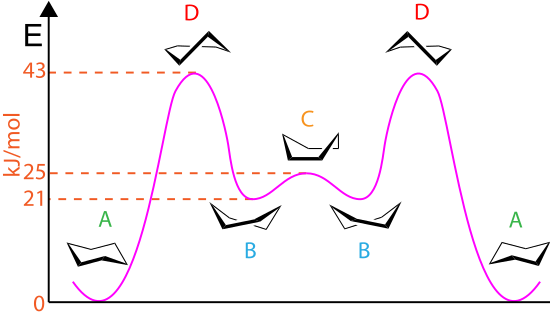
\includegraphics[scale=0.5]{images/cyclohexane_conformations}
		\caption{The conformations of cyclohexane.}
	\end{center}
\end{figure}
\fi
\begin{example}[Moduli space of elliptic curves]\label{}\text{}
A \index{moduli space}moduli space is a space whose points correspond to isomorphism classes of things. (It is tradition to use ``parameter space'' when the thing is embedded in something else and ``moduli space'' otherwise.) An \index{elliptic curve}elliptic curve over $\mathbf{C}$ is a nonsingular curve topologically isomorphic to a torus. Any elliptic curve in the form \[ y^2=x^3+ax^2+bx+c = (x-\alpha) (x-\beta) (x-\gamma).\] One can make some changes of variables to get the elliptic curve into the form
\begin{align*}
	y^2 = x(x-1) (x-\lambda),\ \lambda \ne 0,1.
\end{align*}
(Note that this does not change the isomorphism classes.) One gets the impression that elliptic curves are classified by numbers $\lambda$, but this is invariant under $\lambda\longmapsto 1/\lambda$ and $\lambda \longmapsto 1-\lambda$. Therefore, it is also invariant under
\begin{align*}
	\lambda &\longmapsto \frac{1}{1-\lambda};\\
	\lambda&\longmapsto \frac{\lambda}{\lambda-1};\\
	\lambda&\longmapsto \frac{\lambda-1}{\lambda};
\end{align*}
etc. These six transformations form a group isomorphic to $\Sg_3$. We get this affine variety $\mathbf{A}^1 - \{0,1\}$ modulo $\Sg_3$. This is an affine variety: if $\lambda\in \mathbf{A}^1-\{0,1\}$, one can think of this set as the curve $\lambda(\lambda-1)\mu = 1\subset\mathbf{A}^2$. What is this space $(\mathbf{A}^1 - \{0,1\}) / \Sg_3$, exactly? The coordinate ring is $K[\lambda, 1/\lambda, 1/(\lambda-1)]$, so we consider the subring of this invariant under $\Sg_3$. The simplest invariant element is 
\begin{align*}
	j(\lambda) =  \frac{2^8(\lambda^2-\lambda+1)^3}{\lambda^2(\lambda-1)^2}.
\end{align*}
It turns out that $K[\lambda, 1/\lambda, 1/(\lambda-1)]^{\Sg_3} \isomto K[j]$. This is the so-called \index{$j$-invariant}$j$-invariant of an elliptic curve.
\end{example}


\subsection{Dimension}
Dimension\index{dimension} first was thought of as the number of parameters needed to define a point. However, this fails: Cantor showed that $\mathbf{R}^2$ and $\mathbf{R}$ have the same number of points. Peano and Hilbert showed that there are continuous maps from $\mathbf{R}$ onto $\mathbf{R}^2$. So, in a sense, one does not need two parameters to describe points in $\mathbf{R}^2$. (This does make sense if one looks at smooth manifolds.)

The second attempt was the \index{Lebesgue covering dimension}Lebesgue covering dimension: A set has dimension at most $n$ if every open cover has a refinement such that each point is in at most $n+1$ sets. This works for Euclidean space but isn't all that useful in algebraic geometry.

The next definition is due to Brouwer, Menger, and Urysohn: The boundary of a topological space should have smaller dimension than the topological space. A topological space has dimension at most $n$, then, if all points have arbitrarily small neighbourhoods whose boundary has dimension less than $n$. Traditionally, this definition is used for separable metric spaces, and the spaces one encounters in algebraic geometry are not separable or metrizable. However, this definition works well for definitions of algebraic sets. (This is called \index{inductive dimension}inductive dimension, by the way.) If $\dim$ is the inductive dimension, one has
\begin{align*}
	\dim \emptyset := -1.
\end{align*}

Next, one has the \defn{Krull dimension}\index{Krull dimension}: The supremum of the numbers $n$ for which there is a chain
\begin{align*}
	Z_0\subsetneq Z_1\subsetneq \cdots \subsetneq Z_n
\end{align*}
of irreducible subsets. This only works well for Noetherian spaces. All Hausdorff spaces have Krull dimension $0$. Note that, in the case of Noetherian spaces, the Brouwer--Menger--Urysohn (inductive) dimension is the same as the Krull dimension.

\begin{remark}
	One uses the Krull dimension over the inductive dimension for historical reasons.
\end{remark}

One gets various variations on the \index{Hausdorff dimension}Hausdorff dimension, which is determined by counting the number of balls used to cover a metric space and then seeing what happens to the number of balls as the radii tend to $0$. (Interestingly, Hausdorff dimensions do not need to be integers; they don't need to be rational, either.) It isn't really relevant here, though.

One might consider transfinite dimensions\index{transfinite dimension}. Again, this isn't pertinent here.

One also has the \index{deviation of a poset}deviation of a poset. A poset has deviation at most an ordinal $\alpha$ if, for all descending chains, almost all intervals of the chain have deviation less than $\alpha$. For Noetherian rings, one looks at a poset of ideals; then, the deviation is the Krull dimension. This works well for modules and noncommutative rings. Notice that some posets do not have a deviation: for example, $\mathbf{Q}$. This means that there are some weird non-Noetherian commutative rings that do not have a deviation. (For non-Noetherian rings, there doesn't seem to be a good definition for ``dimension.'')

Now, we move on to algebraic definitions. The idea is that a set of high dimension has many functions on it.

Suppose $B$ is a variety over a field $K$. Look at the field of fractions of the coordinate ring of $B$. Set the dimension of $B$ to be the transcendence degree of the field of fractions. (Recall that the transcendence degree is the largest number of algebraically indepdent elements in the field.) If $B=\mathbf{A}^2$, the coordinate ring is $K[x,y]$, so the field of fractions is rational functions in two variables. This, clearly, has transcendence degree $2$. This works for algebraic varieties, but it doesn't work for more general objects in algebraic geometry: for example, for non-irreducible algebraic sets (which don't have a field of fractions). This doesn't work well for schemes, either: $\Spec \Z$ should have dimension $1$, but this definition gives $0$.

Next, one has the \index{Hilbert polynomial}Hilbert polynomial. This works for local rings $A$. (Recall that a ring is a \index{local ring}local ring if it has a unique maximal ideal $\mathfrak{m}$.) The (length of) dimension $\dim(A/\mathfrak{m}^k)$ is a polynomial in $k$ for large $k$ of degree $d$. Hence, we define $\dim A := d$. Consider the local ring $K [\![x_1,\hdots, x_n]\!]$ which has the maximal ideal $\mathfrak{m} = (x_1,\hdots, x_n)$. The dimension of $A/\mathfrak{m}$ is $1$, of $A/\mathfrak{m}^2$ is $1+n$, of $A/\mathfrak{m}^3$ is $1+n+n(n+1)/2$, etc.

One also considers the Gelfand--Kirillov dimension\index{Gelfand--Kirillov dimension} of a ring, which applies to finitely-generated algebras over a field. It is given by
\begin{align*}
	\limsup_{n} \log \dim R_n / \log n
\end{align*}
where $R_n$ is the subspace generated by monomials in some set of generators of length at most $n$. This isn't of much concern to us, either, since we are concerned with commutative rings and the Hilbert polynomial suffices.

One can define the \index{dimension of the tangent space of a point}dimension of the tangent space of a point of a variety. This works for nonsingular varieties/schemes. For example, if one considers the point $(0,0)$ on the singular curve $y^2=x^3+x^2$, the tangent space will look two-dimensional though you want it to be one-dimensional. However, this is a useful concept because one can define the notion of a singular point with it: a space is nonsingular at a point if the dimension of the tangent space is equal to its dimension.

One can also look at the minimum number of elements in a system of parameters. This works, but it's not intuitive. ``What's a system of parameters?'' A \index{system of parameters}system of parameters for a local Noetherian ring of Krull dimension $d$ with maximal ideal $\mathfrak{m}$ is a set of elements $z_1,\hdots, z_d$ that satisfies these equivalent conditions:
\begin{enumerate}
	\item $\mathfrak{m}$ is a minimal prime over $(z_1,\hdots, z_d)$;
	\item The radical $\sqrt{(z_1,\hdots, z_d)}=\mathfrak{m} $;
	\item Some power of $\mathfrak{m}$ is contained in $(z_1,\hdots, z_d)$;
	\item $(z_1,\hdots, z_d)$ is $\mathfrak{m}$-primary.
\end{enumerate}

Finally, one has various notions of \index{homological dimension}homological dimension.

\subsection{Projective space}
\begin{definition}[ ]\label{}\text{}
\defn{Projective space}\index{projective space} $\mathbf{P}^n(K)$ is the set of all $1$-dimensional subspaces of $K^{n+1}$.
\end{definition}

We use coordinates as follows: $(x_0:x_1:\cdots : x_n)\sim (\lambda x_0:\lambda x_1:\cdots:\lambda x_n)$ where not all $x_i=0$ and $\lambda\in K - \{0\}$.

If $x_0\ne 0$, we can write
\begin{align*}
	(x_0:x_1:\cdots:x_n) = (1:y_1:\cdots : y_n)
\end{align*}
where $y_i = x_i/x_0$. Therefore, $\mathbf{P}^n \supset \mathbf{A}^n$. If $x_0=0$, we get a copy of $\mathbf{P}^{n-1}(K)$. So $\mathbf{P}^n(K)$ is a disjoint union $\mathbf{A}^n(K) \sqcup \mathbf{P}^{n-1}(K) $. We think of the points of $\mathbf{P}^{n-1}(K)$ as ``\index{point at infinity}points at infinity.''

Consider $\mathbf{P}^n(\mathbf{R})$; we have $(x_0:\cdots:x_n)$, which we can rescale such that $x_0^2 +\cdots+x_n^2 = 1$. There are exactly two points, then, corresponding to the same line: $(x_0:\cdots:x_n)$ and $(-x_0:\cdots:-x_n)$. These correspond to antipodal points on the unit sphere. Hence, we have
\begin{align*}
	\mathbf{P}^n(\mathbf{R}) = S^n / \sim
\end{align*}
where $\sim$ identifies antipodal points. One sees that $\mathbf{P}^0(\mathbf{R})$ is a point and $\mathbf{P}^1(\mathbf{R})$ is the unit circle. The space $\mathbf{P}^2(\mathbf{R})$ is the simplest \index{non-orientable surface}non-orientable surface.

Now, consider $(x_0:\cdots : x_n)\in \mathbf{P}^n(\mathbf{C})$. We can rescale this such that $\left\lvert x_0 \right\rvert ^2 + \cdots \left\lvert x_n \right\rvert ^2 = 1$, which gives the sphere $S^{2n+1}$. However, this point is equivalent to $(\lambda x_0:\cdots:\lambda x_n)$ whenever $\left\lvert \lambda \right\rvert =1$, which gives a copy of $S^1$. Thus, we get a map from $S^{2n+1}$ onto $\mathbf{P}^n(\mathbf{C})$ whose fibres are copies of $S^1$. This is a \index{fibration}fibration. For $n=1$, we get $\C \cup \{ \textrm{point}\}$, which is the Riemann sphere (topologically isomorphic to $S^2$). Thus, we get a fibration $S^1 \longrightarrow S^3 \longrightarrow S^2$ (this is the \index{Hopf fibration}Hopf fibration). Another example of a fibration is 
\begin{align*}
	S^1 \longrightarrow S^1\times S^2 \longrightarrow S^2,
\end{align*}
which is the projection onto $S^2$. So $S^3$ is a sort of ``twisted product'' $S^1\times S^2$.


One can cover projective space with copies of affine space. Coordinates of $\mathbf{P}^n(K)$ are given by $(x_0:x_1:\cdots : x_n)$. If $x_0\ne 0$, we get a copy of affine space. Similarly, taking $x_1\ne 0$ gives another copy of affine space. So $\mathbf{P}^n(K)$ is covered by $n+1$ copies of $\mathbf{A}^n(K)$.

Suppose an artist is trying to draw an object---say, a triangle. He must project it onto the plane that is his canvas. What properties are preserved by projection? Parallel lines are not preserved (think of a railway track). Straight lines are preserved, for example.

One can approach geometry in two ways. Synthetic geometry is the axiomatic approach (think Euclid). Analytic geometry is the coordinate approach in which things are translated into algebra. The axioms for projective geometry follow:
\begin{enumerate}
	\item Any two distinct points meet a unique line;
	\item Any two distinct lines in the same plane meet in one point;
	\item Any line meets at least three points.
\end{enumerate}
Dimensions $0$ and $1$ are boring. For dimension $2$, we require any two lines meet at a unique point and any two points lie on a unique line. This is called a projective plane, and there are two types: Desarguesean\index{Desarguesean plane} and non-Desarguesean planes. One example of a projective plane is the Fano plane. 
\begin{figure}
	\begin{center}
		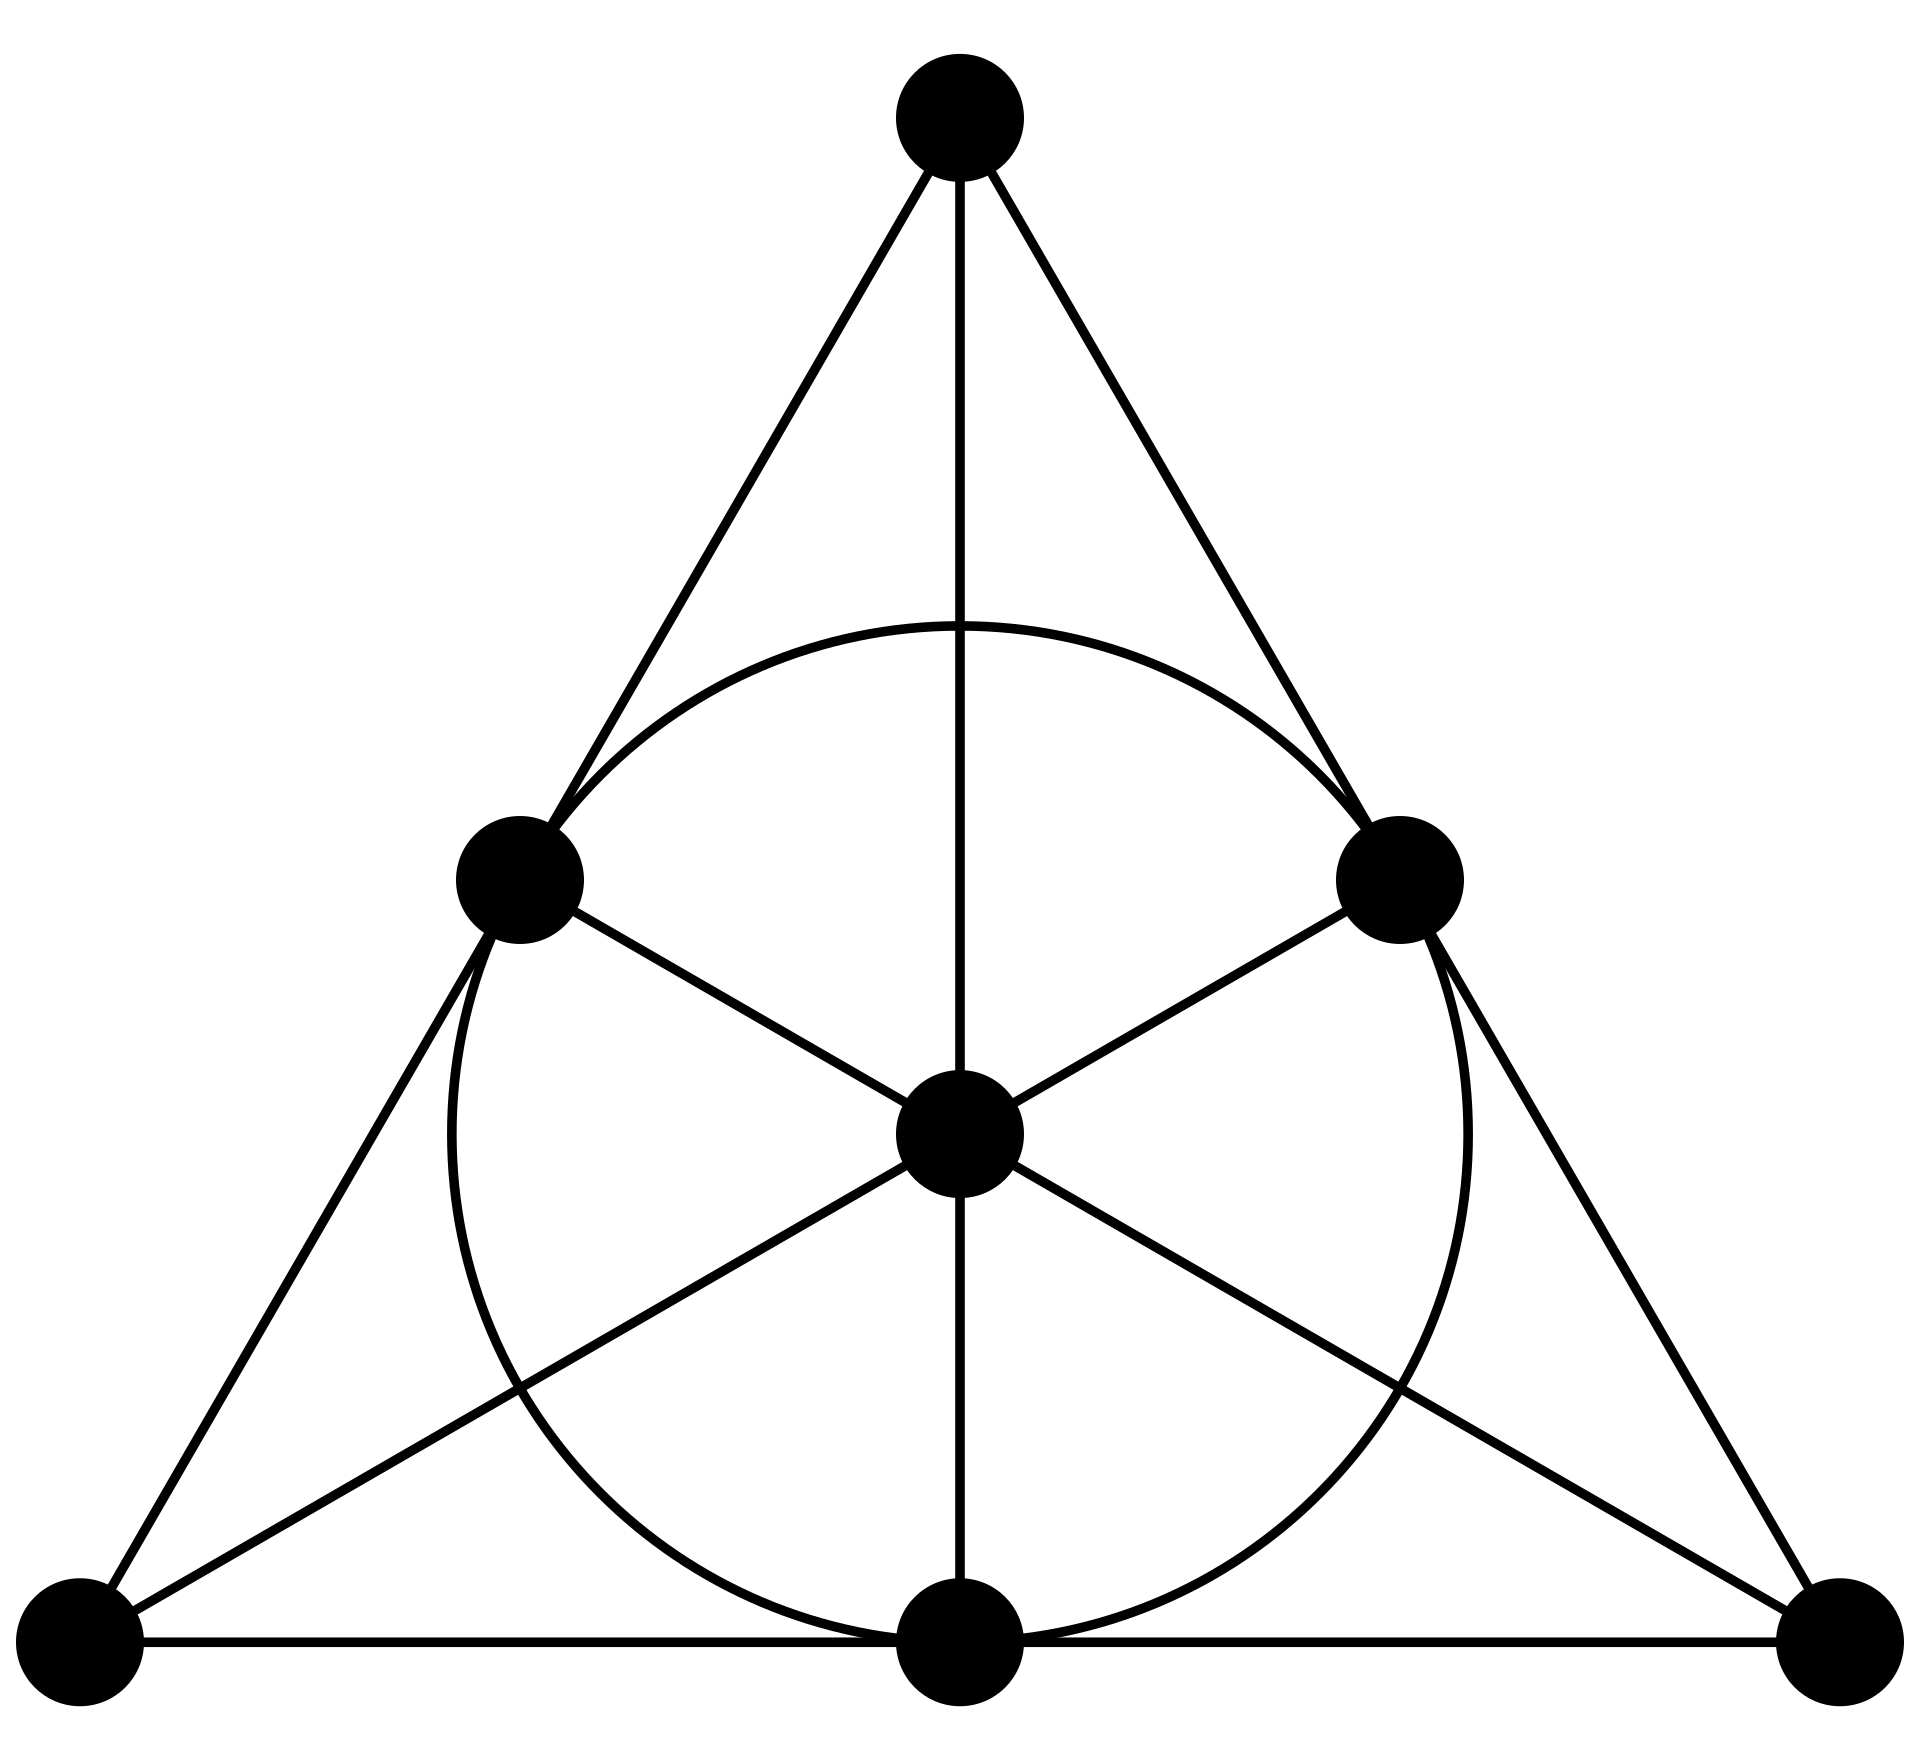
\includegraphics[scale=0.1]{images/fano_plane.png}
		\caption{The Fano plane.}
	\end{center}
\end{figure}
We get plenty of examples for dimension greater than $2$ by taking projective space over a field or division ring. These are all of the examples of projective space in these dimensions. The difference between fields and division rings is that being in a field means that \index{Pappus's theorem}Pappus's theorem holds.

\subsection{Desargues's theorem}
\begin{theorem}[Desargues]\label{}\index{Desargues's theorem}\text{}
If the three straight lines joining the corresponding vertices of two triangles $ABC$ and $\tilde A\tilde B\tilde C$ all meet in a point (the perspector), then the three intersections of pairs of corresponding sides lie on a straight line (the perspectrix). Equivalently, if two triangles are perspective from a point, they are perspective from a line.\footnote{Weisstein, Eric W. ``Desargues's Theorem.'' From \textsl{MathWorld}---A Wolfram Web Resource. \url{https://mathworld.wolfram.com/DesarguesTheorem.html}.}
\end{theorem}
\iffalse
\begin{figure}
	\begin{center}
		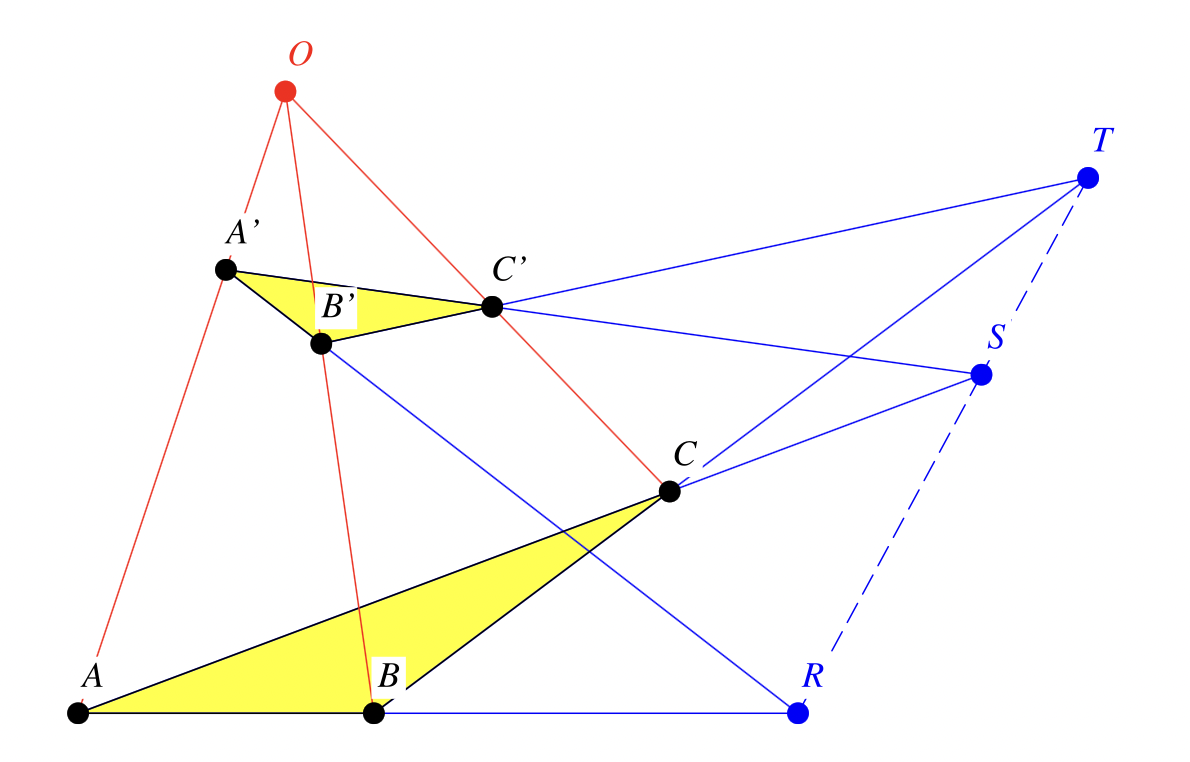
\includegraphics[scale=0.5]{images/desargues}
		\caption{An illustration of Desargues's theorem.}
	\end{center}
\end{figure}
\fi
It is useful to think about these triangles in space. One sees that $AB$ and $\tilde A\tilde B$, $AC$ and $\tilde A\tilde C$, and $BC$ and $\tilde B\tilde C$ do meet. These three points all lie on the planes containing $ABC$ and $\tilde A\tilde B\tilde C$, so they lie on the intersection of these two planes, which is typically a line. ``So, if these triangles are not both contained in the same plane, then Desargues's theorem holds and, if they are contained in the same plane, then you can mumble something about taking limits and still deduce the theorem.''

A projective space automatically satisfies this theorem if it has dimension at least $3$. However, there are some cases in which projective planes do not satisfy it. These counterexamples are called non-Desarguesean planes. In some sense, Desargues's theorem is equivalent to associativity of multiplication. One can introduce coordinates to form a ring for a projective space, and it turns out that the truth of Desargues's theorem is equivalent to associativity holding in the ring, just as Pappus's theorem is equivalent to commutativity. An example of a non-Desarguesean plane is a projective plane over a non-associative ring such as the octonions. (That is, synthetic projective geometry is almost analytic projective geometry, but not quite.)

One also has duality for projective space. Any two distinct points meet in a line, and any two distinct lines meet in a point. That is, points are dual to lines: anything you can say about lines and points you can say about points and lines. There is a dual to Pascal's theorem. 

One can think about this as duality of vector spaces. Points in projective space $\mathbf{P}^n$ correspond to lines in $\mathbf{A}^{n+1}$, which one thinks about as $k^{n+1}$. Lines in $\mathbf{P}^n$ correspond to planes in $k^{n+1}$. Consider the dual space $(k^{n+1})^*$ which is (non-canonically) isomorphic to $k^{n+1}$. The dual of a line in $\mathbf{A}^{n+1}$ is a hyperplane consisting of all linear transformations vanishing on it. So lines correspond to hyperplanes, planes corresponds to things of codimension $2$, etc., so hyperplanes correspond to lines, which are points of projective space.

\subsection{Affine and projective varieties}
Recall that affine space $\mathbf{A}^n$ corresponds to its coordinate ring $k[x_1,\hdots, x_n]$. An affine algebraic subset corresponds to a radical ideal $I=\sqrt{I} $.

Projective space sort of corresponds to $k[x_0,\hdots, x_n]$ where one considers this a graded ring that is graded in the obvious way. Projective algebraic sets correspond\footnote{This correspondence ignores the ideal $(x_0,\hdots, x_n)$.} to graded radical ideals in which every element is a sum of homogeneous elements in the ideal.

A cone over a projective variety in $\mathbf{P}^n$ sort of corresponds to an affine variety in $\mathbf{A}^{n+1}$ invariant under rescaling.

Projective space is affine space together with points at infinity.
\begin{example}[ ]\label{}\text{}
Consider the affine variety $y=x^3$. To make this into a projective variety, instead of considering $(x,y) \in \mathbf{A}^2$, we consider $(x:y:z)\in \mathbf{P}^2$. The affine point $(x,y)$ corresponds to the projective point $(x:y:1)$. We need a homogenous polynomials, so we get $yz^2 = x^3$. What does this variety look like?

Well, $\mathbf{P}^2$ is covered by $3$ copies of affine space, so we can either take $x\ne 0$, $y\ne 0$, or $z\ne 0$. In each case, we scale the nonzero component to make it $1$. If $x=1$, we have $(y,z)$, if $y=1$, we have $(x,z)$, and, if $z=1$, we have $(x,y)$. In the case $z=1$, we get the curve we had before: $y=x^3$. In the case $y=1$, we get $z^2 = x^3$. In the case $x=1$, we get $yz^2 = 1$. One can imagine these three curves, but how do they fit together? 

If we take the point $(1,1)$ on the first curve, this corresponds to $(1:1:1)$ in projective space, which corresponds to $(1,1)$ on the other two curves. The point $(0,0)$ corresponds to $(0:0:1)$. On the second curve, we want to rescale such that $y=1$, but we can't, so this corresponds to a point at infinity, and so it is with the third (here, the point at infinity in the ``rightward'' direction). Now, consider the point $(0,0)$ on the second curve. Again, this corresponds to a point at infinity on the first curve and the other point at infinity on the third one. All other points are on all three curves. Notice that this curve has a singularity at a point at infinity.
\end{example}

\begin{example}[ ]\label{}\text{}
Consider the elliptic curve $y^2 = x^3+bx+c$. This is the affine representation. In the projective plane, we have three coordinates $(x:y:z)$, and we need to make this homogeneous, so we get $y^2z = x^3 + bxz^2 + cz^3$. In the case $z\ne 0$, we get the same curve: $y^2 = x^3 + bx + c$. In the case $z=0$, we get $x=0$, so the only point at infinity is the point $(0:\lambda:0)$. What does the curve look like near this point? Is this singular?

For this, we consider the case $y=1$, so we get $z = x^3 + bxz^2 + cz^3$. The point at infinity in the original curve is the point $(0,0)$ here. If $x$ and $z$ are small, $z$ is $x^3$ plus something small, so around $(0,0)$ we get something that looks like $z=x^3$. So it is nonsingular. So the projective curve is nonsingular at the point at infinity.
\end{example}

\begin{example}[ ]\label{}\text{}
Consider $y^2 = x^2 + 1$. Looking at the curve, one sees that the curve tends to a point where $x$ and $y$ are large and equal to the right, corresponding to $(1:1:0)$. We get another point $(1:-1:0)$. These are points at infinity. A straightforward check corroborates this. 
\end{example}

\begin{example}[Twisted cubic]\label{}\text{}
In affine space $\mathbf{A}^3$, this is the set of points of the form $(t,t^2,t^3)$. The ideal that defines this curve is $(y-x^2, z-x^3)$. What is its closure in projective space $\mathbf{P}^3$?

Here's the wrong answer: Take generators for the ideal and make them homogeneous: We get $ (wy-x^2,w^2z-x^3)$, which is a graded ideal in $k[w,x,y,z]$ and defines something in $\mathbf{P}^3$. The first ideal contains things like $y^2-zx$, but this second one doesn't (it also doesn't contain $z-xy$). In projective space, the closure of the twisted cubic is given by $(s^3:s^2t:st^2:t^3)$ (the curve above where $s=1$ and another point where $s=0$). The ideal of polynomials vanishing on this is $(wy-x^2, y^2-zx, wz- xy)$. What happens if you take the incorrect set of generators for the closure of the twisted cubic?

That is, what happens when one takes $(wy-x^2, w^2z - x^3) \subset k[w,x,y,z]$? What algebraic set in $\mathbf{P}^3$ does it define? Projective space $\mathbf{P}^3$ is covered by four copies of affine space $\mathbf{A}^3$, corresponding to $w=1$, $x=1$, $y=1$, and $z=1$. In the case $w=1$, we get the twisted cubic with which we started. In the case $x=1$, we get $wy=1$ and $w^2z = 1$, which is a copy of the affine $z$-line minus a point (the original curve minus a point). In the case $y=1$, we get $w=x^2$ and $w^2z=x^3$, so $x^3(zx-1)=0$. Hence, we have a curve $zx=1$ which corresponds to the original curve and a triple line where $x=0=w$. That is, what happens when we make this na\"ive choice of generators is that we pick up something strange at infinity.

That this contains two components corresponds to the following decomposition:
\begin{align*}
	(wy-x^2, w^2z - x^3) = (wy-x^2,y^2-xz, wz-xy) \cap  (wy-x^2, w^2, wx).
\end{align*}
\end{example}

\subsection{Products of varieties}
Clearly, one has
\begin{align*}
	\mathbf{A}^m \times \mathbf{A}^n = \mathbf{A}^{m+n}
\end{align*}
where $((x_1,\hdots,x_m),(y_1,\hdots,y_n))\longmapsto  (x_1,\hdots, x_m,y_1,\hdots, y_n)$. In terms of coordinate rings, this is $k[x_1,\hdots,x_m]\tensor_k k[y_1,\hdots, y_n]$, which is more or less $k[x_1,\hdots, x_m,y_1,\hdots, y_m]$. Suppose we have algebraic sets $X$ and $Y$ with corresponding ideals $I$ and $J$. Then $X\times Y$ is the ideal $(I,J)$.

Notice:
\begin{align*}
	\mathbf{P}^m \times \mathbf{P}^n\ne \mathbf{P}^{m+n}.
\end{align*}
This isn't true even topologically: $\mathbf{P}^1(\mathbf{R})\times \mathbf{P}^1(\mathbf{R})\isomto S^1\times S^1$ is the torus, while $\mathbf{P}^2(\mathbf{R})$ is non-orientable. Similarly, $\mathbf{P}^1(\mathbf{C})\times \mathbf{P}^1(\mathbf{C})\isomto S^2\times S^2$ whose second homology group is $\HH^2(S^2\times S^2) =  \mathbf{Z}\oplus \mathbf{Z}$, while $\mathbf{P}^2(\mathbf{C})$ is the union of a point, $\mathbf{C}$, and $\mathbf{C}^2$ whose second homology group is $\mathbf{Z}$. While the convenient equality doesn't hold between these two objects, they are birational.

Let's try to map $((x_0:\cdots:x_m), (y_0:\cdots:y_n))\longmapsto (x_0:\cdots:x_m:y_1:\cdots:y_n)$. Well, this isn't even well defined. To get such a map, we need everything to be of the same degree in $x$ and $y$:
\begin{align*}
	((x_0:\cdots:x_m), (y_0:\cdots:y_n))\longmapsto (x_0y_0:x_1y_0:\cdots:x_my_0:\cdots: x_0y_1:\cdots:x_my_n).
\end{align*}
This gives us the non-surjective map $\mathbf{P}^m\times \mathbf{P}^n\longrightarrow \mathbf{P}^{mn+m+n}$. This is a closed subset. Write an element in the image $(w_{00}:w_{10}:\cdots: w_{m0} : \cdots: w_{mn})$. We have some relations: $w_{ij} = x_iy_j$, so $w_{ij}w_{pq}=w_{iq}w_{pj}$. 

Suppose one has $v\in k^{m+1}$ and $w\in k^{n+1}$. Then one has $v\tensor w \in k^{m+1}\tensor k^{n+1}$. This is, more or less, the map above.

We want to show that the map from $\mathbf{P}^m\times \mathbf{P}^n$ to vectors $(w_{00}:\cdots:w_{mn})$ satisfying $w_{ij}w_{pq}=w_{iq}w_{pj}$ is surjective. One assumes $w_{00}=1$ without loss of generality. Then $w_{pq} = w_{0q}w_{p0}=y_qx_p$. Thus, the $w_{pq}$s are determined by $ w_{0q}$ and $w_{p0}$. We can fix these to be whatever we would like by choosing $x$ and $y$ correctly, assuming $x_0=y_0=1$. Therefore, this map, called the \index{Segre embedding}Segre embedding, is surjective.

\begin{example}[Segre embedding]\label{seg}\text{}
We have
\begin{align*}
	\mathbf{P}^1\times \mathbf{P}^1\longrightarrow \mathbf{P}^{1+1+1}
\end{align*}
given by $((x_0:x_1), (y_0:y_1)) \longmapsto (x_0y_0:x_0y_1: x_1y_0: x_1y_1) =:(w_0:w_1:w_2:w_3)$. We get one relation: $w_0w_3=w_1w_2$. This is a quadric in $\mathbf{P}^3$. Over an algebraically closed field with characteristic not $2$, any two nonsingular quadrics are isomorphic. That is, any quadric in $\mathbf{P}^3$ is isomorphic to $\mathbf{P}^1\times \mathbf{P}^1$. In particular, it has two sets of lines on it. 

Suppose we take a sphere $x^2+y^2+z^2=1$. We claim that this has two sets of straight lines on it. Indeed, it does over $\mathbf{C}$. Example: $x=1$, $y=iz$. Exercise: Find all straight lines on this sphere over $\mathbf{C}$. (Writing this as $(x+iy) (x-iy)= (1-z) (1+z)$ puts into the form of the quadric above.)
\end{example}

\subsection{The Veronese surface and the variety of lines in space}
\begin{example}[Veronese surface]\label{}\text{}
\index{Veronese surface} The Veronese surface is given by
\begin{align*}
	(x^2:xy:xz:y^2:yz:z^2)\in  \mathbf{P}^5.
\end{align*}
One can think of this as a map $\mathbf{P}^2\longrightarrow \mathbf{P}^5$ where
\begin{align*}
	(x:y:z) \longmapsto (x^2:xy:xz:y^2:yz:z^2).	
\end{align*}
This is clearly not surjective. Write this point as $(w_{00}:w_{01}:w_{02}:w_{11}:w_{12}:w_{22})$. One has $w_{ij}w_{pq} = w_{ip}w_{jq}$. Accounting for these relations, the map is surjective. One can also think of this as a map $\mathbf{A}^3\longrightarrow \mathbf{A}^6$ where $\mathbf{A}^6 = \Sigma^2\mathbf{A}^3$ is thought of as the symmetric square of $\mathbf{A}^3$. Note that $\dim \Sigma^2\mathbf{A}^n = n(n+1)/2$. One can also consider maps $\mathbf{A}^3\longrightarrow \Sigma^3 \mathbf{A}^3$ and $\mathbf{A}^m \longrightarrow \Sigma^n \mathbf{A}^m$. The images of these maps are \index{Veronese variety}Veronese varieties.
\end{example}

\begin{example}[Variety of lines in $\mathbf{P}^3$]\label{}\text{}
We expect this variety to be of dimension $4$. A line in $\mathbf{P}^3$ corresponds to a two-dimensional subspace of $k^4$. This is a special case of a \index{Grassmannian}Grassmannian. A Grassmannian $\Gr(m,n)$ is the set of $m$-dimensional subspaces of the vector space $k^{m+n}$. The Grassmannians $\Gr(0,m)=\Gr (m,0)$ are points. The Grassmannian $\Gr(1,m)$ is projective space $\mathbf{P}^m$. Finally, $\Gr(m,n)\isomto \Gr (n,m)$. The first is an $m$-dimensional subspace of $k^{m+n}$; its dual $(k^{m+n})^*\isomto k^{m+n}$ gives an $n$-dimensional subspace. So $\Gr(m,1)\isomto \Gr(1,m)$. The first nontrivial case of this is $\Gr(2,2)$, which is the two-dimensional subspaces of $k^4$.

Grassmannians are special cases of \index{Hilbert scheme}Hilbert schemes: Schemes whose points correspond to certain configurations (algebraic sets, subschemes) of projective space satisfying certain conditions; the simplest condition is that this should be a linear subspace.

We would like to make $\Gr(2,2)$ a projective variety. We shall embed $\Gr(2,2)$ into $\mathbf{P}^5$. Pick a line in $\mathbf{P}^3$ which corresponds to a point of $\Gr(2,2)$. Pick two points $(a_0:a_1:a_2:a_3)$ and $(b_0:b_1:b_2:b_3)$ on the line. Consider the matrix
\begin{align*}
	\mat{a_0&a_1&a_2&a_3\\b_0&b_1&b_2&b_3}.
\end{align*}
Let $S_{ij}$ be the determinant of the columns $i$ and $j$. We get $(S_{01}:S_{02}:S_{03}:S_{12}:S_{13}:S_{23}) \in \mathbf{P}^5$. This point depends on only the line. The map we get is not surjective, since $\Gr(2,2)$ is dimension $4$ and $\mathbf{P}^5$ is dimension $5$. Therefore, there must be a relation between these determinants. This is the \index{Plucker relation}Plucker relation:
\begin{align*}
	S_{01}S_{23}-S_{02}S_{13}+S_{03}S_{12}=0.
\end{align*}
There are no other relations.

We want to show that the map from $\Gr(2,2)$ to solutions to the Plucker relation is surjective. Some $S_{ij}$ must be nonzero, so we can assume it is $1$. Without loss of generality, assume that $S_{01}=1$. Then $S_{01}S_{23}$ is some combination of the other determinants, and $S_{23}$ is determined by them. We get a matrix
\begin{align*}
	\mat{1&0&-S_{12}&-S_{13}\\0&1&S_{02}&S_{03}}
\end{align*}
which gives a line in $\Gr(2,2)$ with image a given point of $\mathbf{P}^5$.
\end{example}

One can use this to find the cohomology of a quadric in $\mathbf{P}^5(\mathbf{C})$. The Grassmannian is a union of subsets:
\begin{align*}
	&\mat{1&0&*&*\\0&1&*&*};\\
	&\mat{1&*&0&*\\0&0&1&*};\\
	&\mat{1&*&*&0\\0&0&0&1};\\
	&\mat{0&1&0&*\\0&0&1&*};\\
	&\mat{0&1&*&0\\0&0&0&1};\\
	&\mat{0&0&1&0\\0&0&0&1}.
\end{align*}\iffalse
\begin{align*}
	&\mat{0&0&1&0\\0&0&0&1}.
\end{align*}
\fi
These correspond to $\mathbf{A}^4$, $\mathbf{A}^3$, $\mathbf{A}^2$, $\mathbf{A}^2$, $\mathbf{A}^1$, and $\mathbf{A}^0$ respectively. One also uses this to determine how many points $\Gr(2,2)$ has over a finite field $k$. If $q=\left\lvert k \right\rvert $, then $\Gr(2,2)$ has $q^0 + q^1 + 2q^2 + q^3+q^4$ points. One sees that $\mathbf{P}^4$ has $q^0+q^1+q^2+q^3+q^4$ points.

This strongly suggests there is a relationship between the cohomology groups of a variety over $\mathbf{C}$ and the number of points of that variety over a finite field. This is the concern of the Weil conjectures.

\subsection{Grassmannians}
The Grassmannian $\Gr(2,2)$ can be thought of as the two-dimensional subspaces of $k^4$, or, alternatively, lines in space. Grassmannians $\Gr(m,n)$ are injective maps $k^m \longrightarrow k^{m+n}$.
One can show that
\begin{align*}
	\Gr(m,n) \subseteq  \mathbf{P}^{\binom{m+n}{m}-1}.
\end{align*}

Suppose we are given an $m$-dimensional subspace of $k^{m+n}$. Pick $m$ vectors spanning it. This gives an $m\times(m+n)$ matrix:
\begin{align*}
	\mat{a_1&\cdots &a_{m+n}\\b_1&\cdots &b_{m+n}\\&\vdots}.
\end{align*}
Pick any $m$ columns and consider the determinant of these columns. This generates $\binom{m+n}{m}$ numbers. Call them $p_{{i_1},\hdots,{i_m}}$. These give a point in $\mathbf{P}^{\binom{m+n}{m} - 1}$. 

Instead, suppose $V\subseteq W$ is a subspace of $W$ with with dimension $m$. Suppose $W$ has dimension $m+n$. Then we have a map from the $m$th exterior power of $V$ to the $m$th exterior power of $W$:
\begin{align*}
	\Lambda^m V \longrightarrow  \Lambda ^m W.
\end{align*}
The first space has dimension $1$ and the second has dimension $\binom{m+n}{m}$. A one-dimensional subspace of something corresponds to the projective space of that thing: $\mathbf{P}(\Lambda^m W)$. This map is not surjective. We have the Plucker relations:
\begin{align*}
	0 &= \sum_{\lambda}^{} (-1)^\lambda p_{i_1,\hdots, i_{m-1},j_\lambda} p_{j_1,\hdots, j_{\lambda -1},j_{\lambda+1},\hdots, j_{m+1}}.
\end{align*}
These give quadric relations that make the map from $\Gr(m,n)$ to the roots of the Plucker relations surjective. We can assume, say, that $p_{1,\hdots, m} = 1$. Then, we can find a point of $\Gr(m,n)$ with given values of $p_{1,\hdots, r-1,r+1,\hdots, m,s}$. The Plucker relations determine all of the other $p$s.

Grassmannians have applications.
\begin{enumerate}
	\item Grassmannians are covered by affine spaces that can be used to determine their cohomologies.
	\item One has the Littlewood--Richardson rule\index{Littlewood--Richardson rule} that gives the product of the cohomology of a Grassmannian.
	\item One has \index{line complex}line complexes. The quadric line complex is given as follows. Take $\Gr(2,2)\subset  \mathbf{P}^5$. Intersect $\Gr(2,2)$ with a quadric.
	\item The Grassmannian $\Gr(m,n)$ is a quotient \[\frac{\GL_{m+n}(k)}{\mat{*&*\\0&*}}.\] The group $\GL_{m+n}(k)$ is affine and the second is, too, though $\Gr(m,n)$ is not affine; it is projective, however. Quotients of affine varieties do not need to be affine or projective: take 
		\begin{align*}
			k^2 - (0,0) =  \frac{\GL_{2}(k) }{\mat{1&*\\0&1}}.
		\end{align*}
	\item Grothendieck used Grassmannians in his construction of Hilbert schemes. A \index{Hilbert scheme}Hilbert scheme parameterizes subschemes of projective space: Take the coordinate ring $k[x_0,\hdots, x_n]$ of projective space and consider graded ideals $I = \bigoplus_j I_j$. Subschemes sort of correspond to graded ideals, so one tries to classify graded ideals and show that they correspond to points of a projective scheme. The dimension $\dim (I_j)$ is a polynomial in $j$ for $j$ large. Suppose $I_d$ generates $I_{d+1},I_{d+2},\hdots$. Then $I_d \subseteq S_d$ (degree $d$ monomials). This gives a point of a Grassmannian, which is itself a projective variety in a larger projective space.
\end{enumerate}

We would like to say that lines in $\mathbf{P}^3$ ``naturally'' correspond to points of $\Gr(2,2)\subset  \mathbf{P}^5$. What does ``natural'' mean? Grothendieck looked at functors from commutative rings $R$: maps $F$ from $R$ to lines in $\mathbf{P}^3(R)$, maps from $R$ to $\Gr(2,2)$ over $R$, maps $G$ from $R$ to $R$-valued points of a quadric given by the Plucker relation. Grothendieck showed that these are isomorphic as functors. Suppose $\phi: R\longrightarrow  S$ is a ring homomorphism. Then we have maps $F(R) \longrightarrow F(S)$ and $G(R) \longrightarrow G(S)$ that make this commute:
\[
\begin{tikzcd}
F(R) \arrow[d, -,double equal sign distance,double]\arrow[r] &F(S) \arrow[d, -,double equal sign distance,double] \\ G(R)\arrow[r] & G(S).
\end{tikzcd}
\]
Grothendieck showed that any scheme is defined by its functors of points.

\subsection{Projective space bundles}
Recall the definition of a fibre bundle: A fibre bundle\index{fibre bundle} is a space that looks like a product locally. Specifically, a fibre bundle is a structure $(E,B, \pi, F)$ where $E$, $B$, and $F$ are topological spaces and $\pi:E\longrightarrow B$ is a continuous surjective map that, in small regions of $E$, behaves like a projection from $B\times F$ to $B$. For sufficiently small open sets $U$:
\begin{center}
	\begin{tikzcd}
		F \ar[r] & E\ar[d] & F\times U \ar[d]\\
			 &B&U\ar[l,hook'].
	\end{tikzcd}
\end{center}

Take $B=S^1$ and $F=\mathbf{R}$. Then we can map $S^1\times \mathbf{R}$ onto $S^1$, which would look like a cylinder mapping onto a circle with fibres copies of $\mathbf{R}$. One can twist this construction, mapping a M\"obius strip onto $S^1$. One can think of the fibres as copies of $\R$. Locally, this looks like a product: The preimage of a little section of the circle looks like $\R$ times that little section.

Fibre bundles are ``twisted products.'' Often, the fibre is a vector space; in this case, we talk about a \index{vector bundle}vector bundle. If the fibre is a copy of projective space, we talk about a \index{projective space bundle}projective space bundle.

\begin{example}[Hirzebruch surface]\label{}\text{}
\index{Hirzebruch surface}Consider the space
\begin{align*}
	(\mathbf{A}^2 - \{0\}) \times (\mathbf{A}^2 - \{0\}).
\end{align*}
Act on this by $G_m\times G_m$; think of $G_m$ as $\mathbf{C}^*$. The quotient $(\mathbf{A}^2 - \{0\})/G_m$ where $\lambda \in G_m$ acts by $(x,y)\longmapsto  (\lambda x,\lambda y)$ is the projective line $\mathbf{P}^1$. Pick a point $(\lambda,\mu)\in  G_m\times G_m$; now, act on a point $(s,t,x,y)$ by
\begin{align*}
	(s,t,x,y)\longmapsto  (\lambda s, \lambda t,\mu x,\lambda^{-\alpha}\mu y),\ \alpha\in  \mathbf{Z}.
\end{align*}
The quotient defined by this action is a Hirzebruch surface. One has a map
\begin{align*}
	F := \frac{(\mathbf{A}^2-\{0\})\times (\mathbf{A}^2-\{0\})}{G_m\times G_m} \longrightarrow \mathbf{P}^1
\end{align*}
given by
\begin{align*}
	(s,t,x,y)\longmapsto  (s:t).
\end{align*}
The fibre at any point is also isomorphic to $\mathbf{P}^1$. This is a product locally, but it isn't globally. We have a surface that is a fibre bundle over $\mathbf{P}^1$ with fibres also $\mathbf{P}^1$.
\end{example}

\begin{example}[Scroll]\label{}\text{}
\index{scroll}Act on the space
\begin{align*}
	(\mathbf{A}^2- \{0\}) \times (\mathbf{A}^n - \{0\})
\end{align*}
by $G_m\times G_m$ where $(\lambda,\mu)$ acts on $(s,t,x_1,\hdots, x_n)$ by 
\begin{align*}
	(s,t,x,y)\longmapsto  (\lambda s, \lambda t, \lambda^{-\alpha_1}\mu x_1,\hdots, \lambda^{-\alpha_n}\mu x_n), \ \alpha_i\in \mathbf{Z}.
\end{align*}
We get a map from the scroll to the projective line: 
\begin{align*}
	\frac{(\mathbf{A}^2-\{0\}) \times (\mathbf{A}^n-\{0\})}{G_m\times G_m} \longrightarrow \mathbf{P}^1
\end{align*}
given by
\begin{align*}
	(s,t,x_1,\hdots, x_n) \longmapsto (s:t).
\end{align*}
Here, the fibres are copies of $\mathbf{P}^{n-1}$. Grothendieck showed that, if one has a vector bundle over the projective line,  one can replace each vector space that is a fibre with the corresponding vector space, and this gives a projective bundle over $\mathbf{P}^1$. This construction covers all such vector bundles.

Let us map this to projective space. Assume that all of the $\alpha_i>0$. Consider the monomials $s^it^{\alpha_j-1}x_j$. One can take these as the coordinates of a point in $\mathbf{P}^{\left( \sum_{}^{} \alpha_j+1 \right) - 1}$.
\end{example}

\index{abstract variety}Abstract varieties were invented by Andr\'e Weil to take the Jacobian of a curve to formulate his Weil conjectures. A differentiable manifold was viewed as a subset of $\mathbf{R}^n$ defined by some equations. For instance, $S^2$ is the set of points $x^2+y^2+z^2=1$ in $\mathbf{R}^3$. However, this isn't a differentiable manifold, really; it is a differentiable manifold together with an embedding into Euclidean space. Now, one covers $S^2$ with charts\index{chart}: a top hemisphere and a bottom hemisphere, each of which looks like an open disk in Euclidean space, glued together. 

The old view was that a variety is a subset of $\mathbf{P}^n$ defined by equations. The new one: Take some affine varieties and glue them together. One might have considered $\mathbf{P}^1$ as a subset of projective space (itself). Alternatively, one can glue together two copies of $\mathbf{A}^1$, so $\mathbf{P}^1=\mathbf{A}^1\cup \mathbf{A}^1$. The projective line is given by $(x:y)$, the first copy of $\mathbf{A}^1$ is given by $(1:y)$, and the second is given by $(x:1)$. For both copies, we consider the subset $\mathbf{A}^1-\{0\}$. Then, if we have $x$ in the first copy and $y$ in the second, we map 
\begin{align*}
	x\longmapsto \frac{1}{y}.
\end{align*}
The ``gluing'' given by $x\longmapsto y$ is kind of funny: you get a line with two origins; this is a non-Hausdorff manifold and a non-projective abstract variety. If one eliminates this phenomenon, all dimension-$1$ abstract varieties are projective. One needs to exclude singularities in dimension $2$. There are some abstract nonsingular non-projective varieties in dimension $3$. \index{Chow's lemma}Chow's lemma says that an abstract complete variety is pretty close to a projective variety. 

\subsection{Toric varieties}
\index{toric variety}Toric varieties give an easy way to construct examples of projective varieties.

\begin{example}[Constructing affine varieties from cones: dimension $2$]\label{}\text{}
Consider the coordinate ring of $k^*\times k^*$, namely $k[x,x^{-1},y,y^{-1}]$. One gets a square lattice of monomials. One defines subrings by drawing cones:
\begin{center}
	\phantom{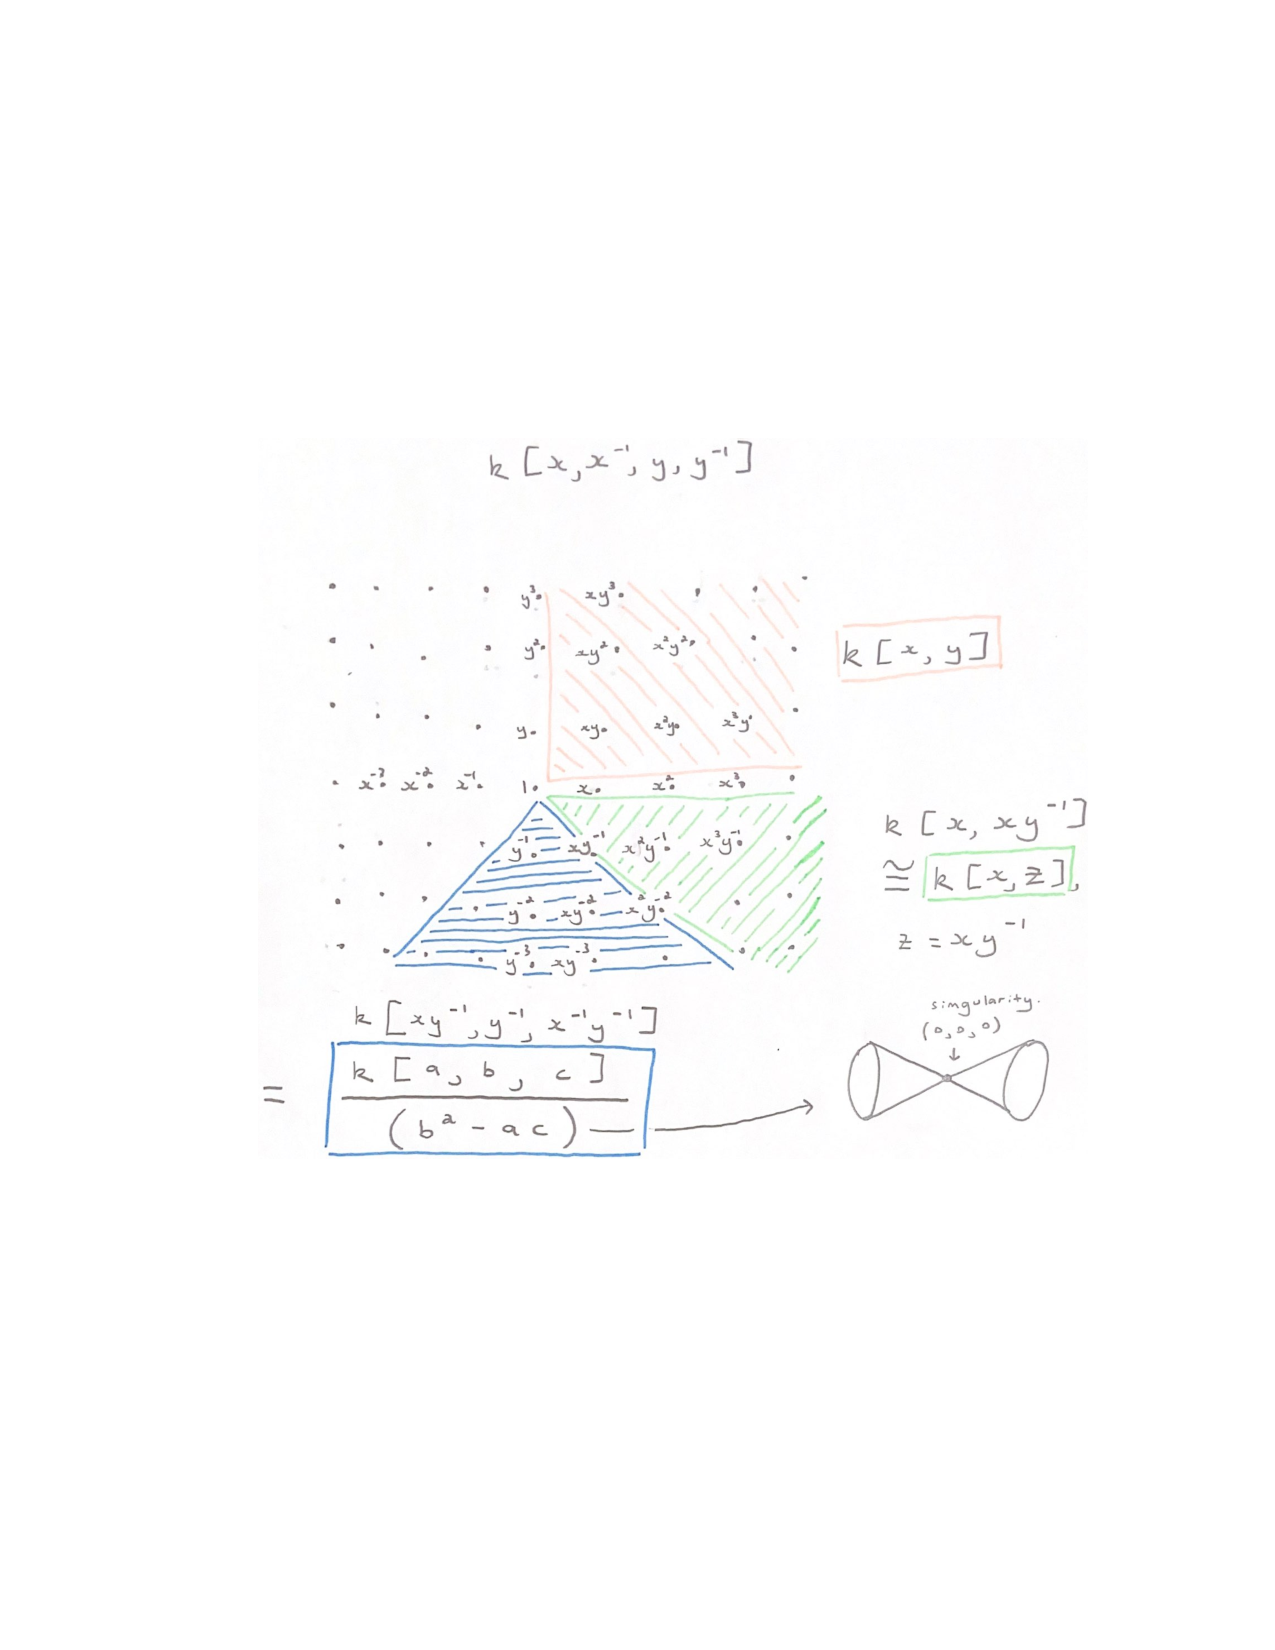
\includegraphics[scale=0.8]{images/subring_cone.pdf}}
\end{center}
A subring given by a cone has the following properties:
\begin{enumerate}
	\item It is a $k$-algebra;
	\item It has no nilpotent elements;
	\item If the cone is rational, it is a finitely-generated algebra.
\end{enumerate}
If these three conditions are met, this gives the coordinate ring of an affine variety. The orange and green cones correspond to $\mathbf{A}^2$ and the blue cone corresponds to a double cone as drawn above. 

Suppose we have an orange cone and a larger red cone that contains the orange cone. One sees that the orange ring is a subring of the red ring. Since we have a map from the orange ring to the red ring, we have a map from the red variety to the orange variety. We can get around this problem using duality. 

If one has a cone in $\mathbf{Z}^2$, one can look at the dual cone: the corresponding cone in $(\mathbf{Z}^2)^*=\mathbf{Z}^2$. The orange dual cone contains the red dual cone. The idea: For each cone $C$ in $\mathbf{Z}^2$, look at the dual cone and take the corresponding ring. This gives a variety of $C$.

Consider a degenerate cone (a vertical line). The dual of this cone is the upper half plane. The coordinate ring of this is $k[x,x^{-1},y]$, which corresponds to $k^*\times k$. This is the ring corresponding to the line.

Consider a quadrant. Its dual is the same quadrant whose coordinate ring is $k[x,y]$, so this corresponds to the affine plane or $k\times k$. Now, one sees that sub--- is preserved under taking coordinate rings of cones. (That is, $k^*\times k$ is a subring of $k\times k$ and, correspondingly, the line is a subcone of the quadrant.)
\end{example}

		One can do the same with more cones. Consider the following cones in $1$ dimension: An upward line at the origin, a downward line at the origin, and their intersection (a point). The lines are self-dual, but the dual of the point is the entire line. The lines correspond to $k[x]$ and $k[x^{-1}]$ respectively, thus $\mathbf{A}^1$, and the point corresponds to $k[x,x^{-1}]$, thus $\mathbf{A}^1 - \{0\}$. Take these affine varieties and glue them together. One gets $\mathbf{P}^1$. 


Now, in two dimensions, take four distinct quadrants. One gets four varieties which are isomorphic to $\mathbf{A}^2$. We are gluing them together along various subvarieties. The right horizontal one corresponds to $\mathbf{A}^2 - \mathbf{A}^1 = \mathbf{A}^1 \times (\mathbf{A}^1 - \{0\})$. The picture we have is just two copies of the picture we had in the one-dimensional case, so we get $\mathbf{P}^1\times \mathbf{P}^1$. The variety $\mathbf{P}^1 \times \mathbf{P}^1$ as a toric variety is drawn like this. How do we get $\mathbf{P}^2$?

Consider these cones:
\begin{center}
	\phantom{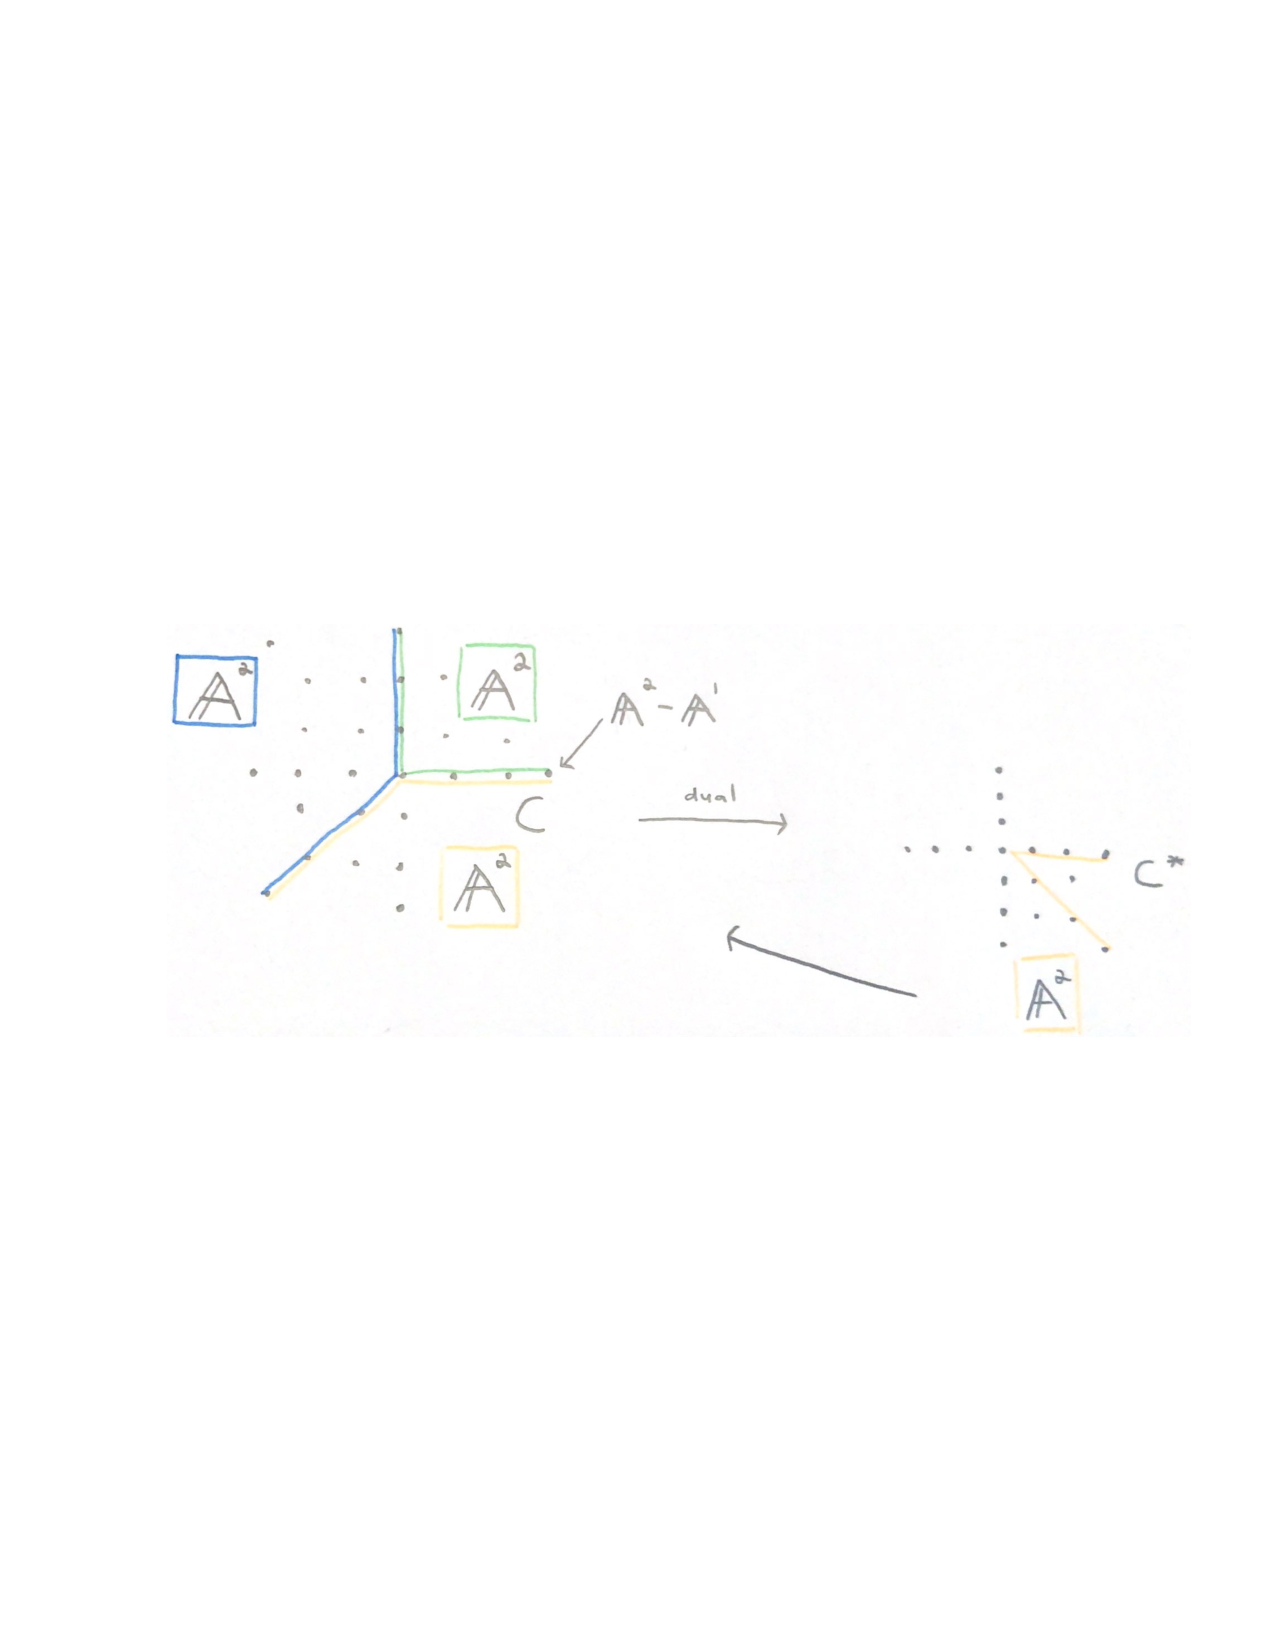
\includegraphics[scale=0.8]{images/toric_proj_plane.pdf}}
\end{center}
Looking at the dual cone, we see that the orange and blue cones correspond to $\mathbf{A}^2$.  Again, we see that the green and orange cones are glued together by the variety $\mathbf{A}^2 - \mathbf{A}^1$. So $\mathbf{P}^2$ is $\mathbf{A}^2\cup \mathbf{A}^2\cup \mathbf{A}^2$ glued along copies of $\mathbf{A}^1\times (\mathbf{A}^1-\{0\})$.

Consider this more exotic example:
\begin{center}
	\phantom{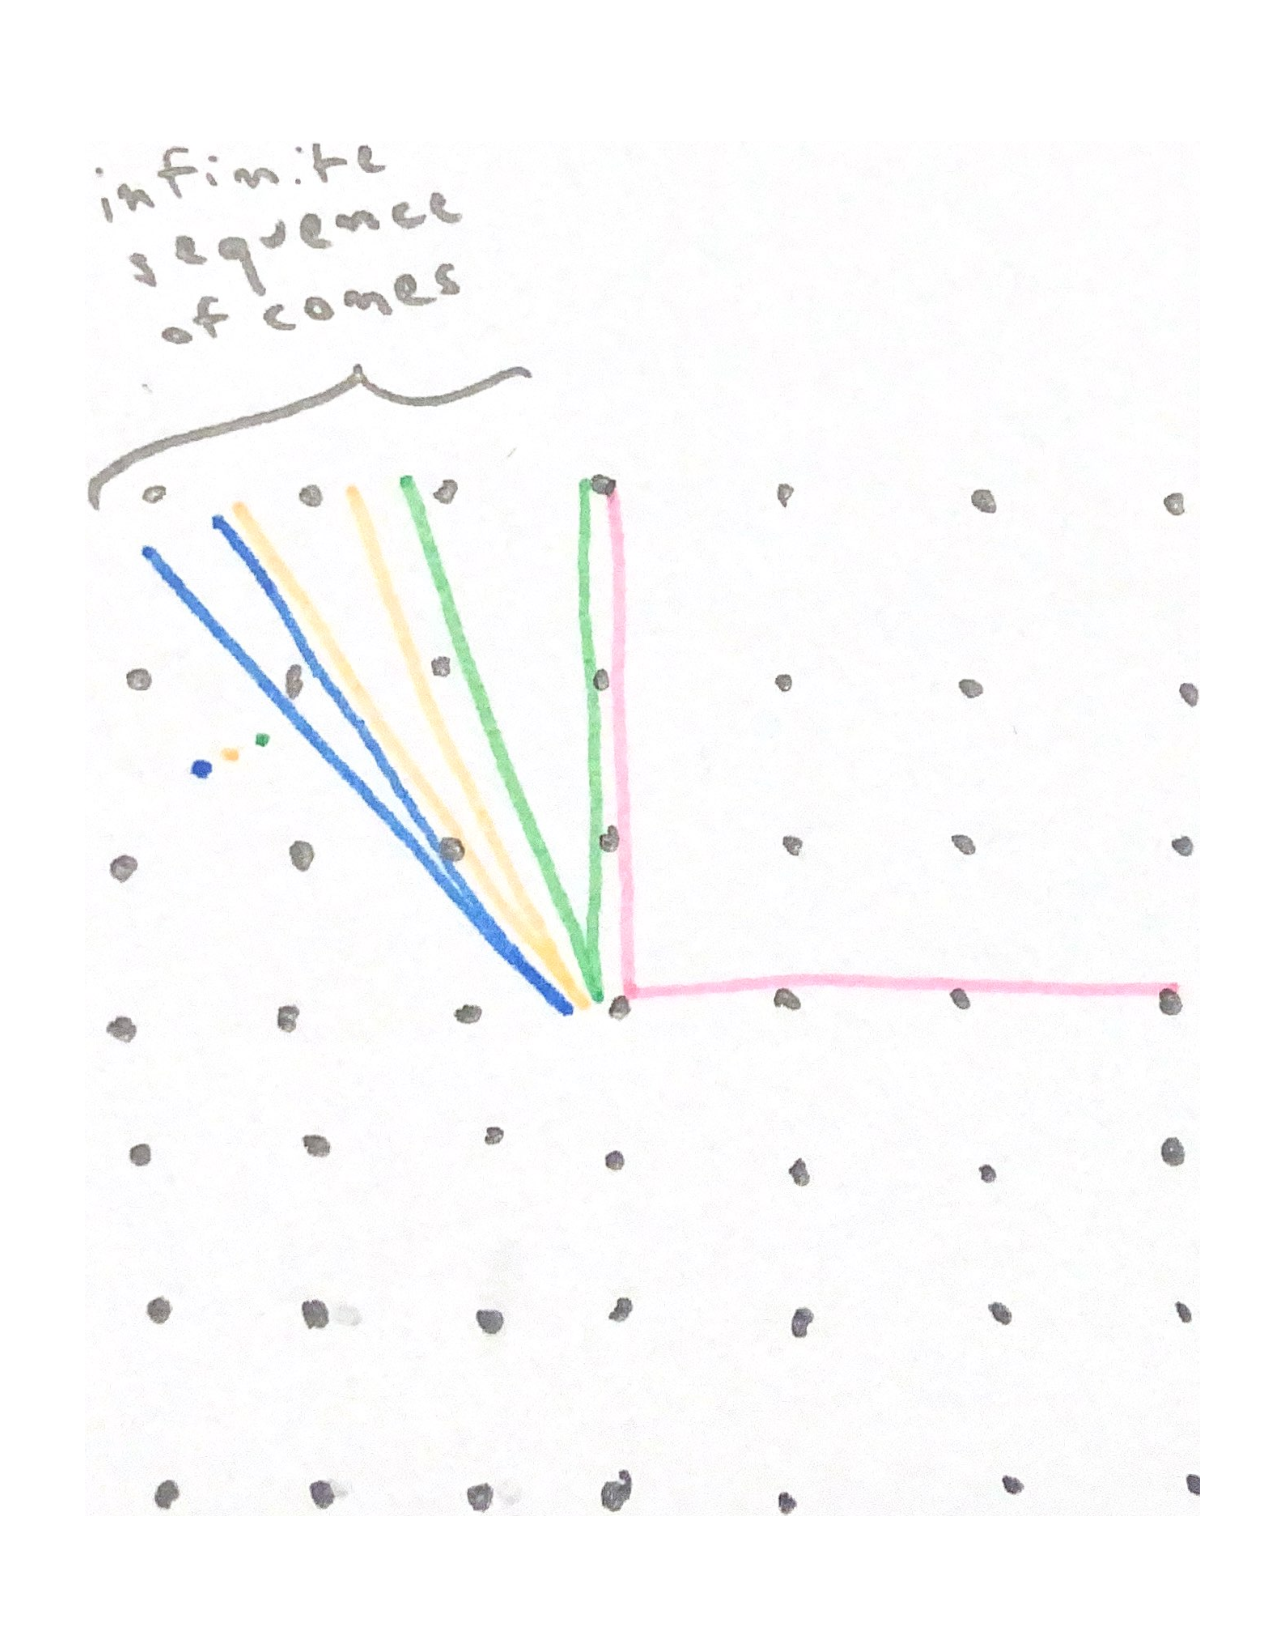
\includegraphics[scale=0.4]{images/cone_seq}}
\end{center}
One can take an infinite sequence of cones and glue together copies of $2$-dimensional affine space according to this sequence. What projective variety does one get? Well, one doesn't get one: It is too big. The resulting thing is not \index{quasicompact}quasicompact, and all projective varieties or their open subsets are quasicompact. Instead, it gives an \index{abstract variety}abstract variety. Varieties one gets like this are called toric varieties: They contain a torus as a dense subvariety.

In the drawing above, notice that there is a single point contained in all of the cones. The variety of this point is, looking at the dual cone, $k[x,x^{-1},y,y^{-1}]$. This is the coordinate ring of a torus. Why is this called a torus?

One knows that, in algebraic topology, a torus is $S^1\times S^1$, or, more generally, $(S^1)^n$. Over $\mathbf{R}$, $S^1$ is the set of points $x^2 + y^2 = 1$. Over $\mathbf{C}$, this is $(x+iy) (x-iy)=1$ or $z_1z_2=1$. This is a hyperbola, which is $\mathbf{C}-\{0\}$. Hence, one can think of $\mathbf{C}^*$ as an analogue of $S^1$. Therefore, one can call $(\mathbf{C}^*)^n$ a torus. In the theory of algebraic groups, $(\mathbf{C}^*)^n$ plays the same role that $(S^1)^n$ plays is the theory of compact Lie groups. 

\subsection{Categories}
A category has objects and morphisms. They are named after their objects. Here are some examples.
	\begin{center}
\begin{tabular}{cc}
    Objects & Morphisms\\
    \midrule
    Sets & Functions\\
    Groups & Group homomorphisms\\
    Topological spaces & Continuous maps\\
    Commutative rings & Ring homomorphisms
\end{tabular}
\end{center}
A category has a collection of objects. For any two objects, one has a collection of morphisms between them. Given objects $A$, $B$, and $C$, a morphism $f$ from $A$ to $B$, and a morphism $g$ from $B$ to $C$, one has a morphism $g\circ f$ from $A$ to $C$. For every object $A$, there is an identity morphism $I_A$. This identity must behave as one expects. Composition of morphisms must be associative when defined.

A theme of category theory is to focus on morphisms between objects, and not the objects themselves. How does one define products? The definitions of products of sets, groups, topological spaces, etc. are notably different. Suppose $A$ and $B$ are two objects. Suppose $C$ is another object with morphisms to $A$ and $B$. Then there is a unique morphism from $C$ to $A\times B$. This is universal:
\begin{center}
	\begin{tikzcd}
		C \ar[ddr] \ar[dr, dashed] \ar[drr] \\
		& A\times B \ar[r] \ar[d] & B\\
		& A
	\end{tikzcd}
\end{center}
One can check that products of sets, groups, rings, topological spaces, etc. satisfy this universal property. The product is not unique but it is unique up to unique isomorphism.

Suppose $X$ and $Y$ both satisfy the universal property above. Since $Y$ is a product and $X$ maps to $A$ and $B$, there is a unique map from $X$ to $Y$ that makes the diagram commute. Reverse the roles of $X$ and $Y$ to get a unique map from $Y$ to $X$. The composition of these two unique morphisms is a map from $Y$ to itself that makes the diagram commute; by unicity, this morphism must be the identity of $Y$. Reverse the roles of $X$ and $Y$.

We would like to make varieties or algebraic sets into a category. One can use \index{regular map}regular maps, which are somewhat analogous to smooth maps in differential geometry and defined everywhere, or one can use \index{rational map}rational maps, which are not defined everywhere.

Given a category $\mathcal{C} $, its opposite $\mathcal{C}\op$ is $\mathcal{C} $ with all arrows reversed. The morphisms of ${\mathcal{C}}\op $ from $A$ to $B$ are the same as the morphisms of $\mathcal{C} $ from $B$ to $A$. Affine varieties with regular maps is somewhat dual to finitely-generated algebras over $k$ with no nilpotent elements. (Affine schemes have the same correspondence to commutative rings.)

A map of varieties $V\longrightarrow W$ does not give a map from a coordinate ring of $V$ to that of $W$; it gives a map from functions on $W$ to functions on $V$.


\subsection{Regular functions}
An affine variety $Y\subseteq \mathbf{A}^n$\index{affine variety} is defined by an ideal $I$ and the coordinate ring of $Y$ is $k[x_1,\hdots,x_n]/I$, which one thinks of as polynomial functions on affine space restricted to $Y$. This coordinate ring is the \index{ring of regular functions}ring of regular functions on $Y$.

We would like to define regular functions when $U$ is an open subset of an affine variety $Y$. Such open sets are called \index{quasiaffine variety}quasiaffine varieties.

\begin{example}[Quasiaffine varieties]\label{}\text{}
Take $U=\mathbf{A}^1-\{0\}$. We have seen that $U$ is isomorphic to the hyperbola of points $xy=1$ in $\mathbf{A}^2$. This quasiaffine variety is an affine variety disguised.

Take $U=\mathbf{A}^2-\{(0,0)\}$. We will see that this is not isomorphic to an affine variety.
\end{example}

What do we want the regular functions on $U$ to be? If $U=\mathbf{A}^1-\{0\}$, we want $x^{-1}$ to be regular on $U$. Hence, we want the ring to be $k[x,x^{-1}]$. We define a regular function\index{regular function} on $U$ to be a function that is locally regular at all points $p\in U$. (A function $f$ is \index{locally regular}locally regular at $p$ if $f=g/h$ in some neighbourhood of $p$ where $g$ and $h$ are polynomials and $h$ is nonzero at $p$. Note that $g$ and $h$ depend on $p$.) 

\begin{problem}
	Suppose $Y$ is affine. Are regular functions regular? Note that the first ``regular'' means ``regular at each point'' and the second means that they are polynomials on affine space.
\end{problem}

Suppose $Y=U_1\cup U_2\cup \cdots \cup U_m$ is a union of open subsets. Let $f$ be a function on $Y$ that is regular on all $U_i$s. Therefore, $f=g_i/h_i$ on $U_i$ where $h_i\ne 0 $ on $U_i$. Is $f$ a polynomial? Observe that $1= a_1h_1 + a_2h_2 + \cdots +a_mh_m\pmod I$ for some polynomials $a_i$. This is because $Y$ is covered by the $U_i$s; thus, no point of $Y$ is outside of all $U_i$s, and no maximal ideal of $k[x_1,\hdots,x_n]$ containing $I$ contains all of the $h_i$s; so $(h_1,h_2,\hdots, h_m, I)=(1)$. This relation gives
\begin{align*}
	f &= a_1h_1f + a_2h_2f + \cdots + a_mh_mf \pmod I\\
	  &= a_1g_1 + a_2g_2+\cdots + a_mg_m \pmod I.
\end{align*}
Define $f:= a_1g_1+\cdots + a_mg_m$. We want to check that $h_if = g_i$ on $U_i$: Since $h_if = h_ia_1g_1 +\cdots + h_ia_mg_m$ and $h_ig_j = h_jg_i$, one gets
\begin{align*}
	h_if &= h_ia_1g_1 +\cdots + h_ia_mg_m\\
	     &= g_ia_1h_1 + \cdots + g_ia_mh_m\\
	     &= g_i(a_1h_1+\cdots+a_mh_m)\pmod I\\
	     &= g_i \pmod I.
\end{align*}
Therefore, the local and global conditions for regularity are equivalent.

Suppose $U$ is a \index{quasiprojective variety}quasiprojective variety, so it is an open subset of a projective variety. (Every quasiaffine variety is a quasiprojective variety.) Notice that a quasiprojective variety is covered by open affine subvarieties. A function on a quasiprojective variety is  \index{regular function}regular if it is \index{locally regular}locally regular.

Given a quasiprojective variety $Y$, one has a \index{ring of regular functions}ring of regular functions $\mathscr{O}(U)$ for each open subset $U\subset Y$. 

Suppose $U= U_1\cup U_2\cup \cdots$. One has the following properties:
\begin{enumerate}
	\item If $f\in \mathscr{O}(U) $ vanishes on $\mathscr{O}(U_i) $, then $f = 0$;
	\item If $f_i\in \mathscr{O}(U_i) $ and $f_i = f_j$ on $U_i\cap U_j$, then there exists $f\in \mathscr{O}(U) $ such that $f \big |_{U_i} = f_i$.
\end{enumerate}
These are the defining conditions of a \index{sheaf}sheaf.

\begin{example}[ ]\label{}\text{}
Let us find the regular functions on $\mathbf{P}^1$. The regular functions on $\mathbf{A}^1$ is $k[x]$. We cover the projective line with two copies of the affine line: $\mathbf{P}^1 = \mathbf{A}^1\cup \mathbf{A}^1$. To specify a regular function $f\in \mathbf{P}^1$, pick regular functions on $\mathbf{A}^1$ and $\mathbf{A}^1$ that are the same on the intersection $\mathbf{A}^1-\{0\}$. The ring of regular functions on $\mathbf{A}^1-\{0\}$ is $k[x,x^{-1}]$. One can identify the ring of regular functions of the second copy of $\mathbf{A}^1$, $k[y]$, with $k[x^{-1}]$. We need to pick $f$ that is a polynomial in $x$ and a function that is a polynomial in $x^{-1}$ that are the same in $k[x,x^{-1}]$. Thus, $f$ is constant.
\end{example}

\subsection{Morphisms of varieties}
Suppose $X$ and $Y$ are quasiprojective varieties. We want to define a regular map $f:X\longrightarrow Y$. This should be a ``nice'' function from points of $X$ to points of $Y$. ``Nice'' functions from $h:Y\longrightarrow k$ are regular functions, so the composition $h\circ f$ should be regular.

Suppose $U$ is open in $Y$. Then $f^{-1}(U)$ is open in $X$. Let $g: U\longrightarrow k$ be a regular function. Then $f$ is called a morphism if the composition $g\circ f$ is regular on $f^{-1}(U)$. Indeed, the composition of two morphisms is a morphism. Quasiprojective varieties and this morphism comprise a category.

\begin{warn}
	This is a morphism of \index{ringed space}ringed spaces. A \defn{ringed space}\index{ringed space} is a topological space with a sheaf of rings. We have seen that regular functions on open sets form a sheaf of rings. This definition fails for schemes: one needs to use a morphism of locally ringed spaces.
\end{warn}

\begin{example}[Ringed spaces]\label{}\text{}
	 Topological manifolds: Take continuous functions on every open set. Then, one can take $C^1$ manifolds, $C^2$ manifolds, etc., and $C^\infty$ manifolds (smooth manifolds), in which the ringed space structure is given by smooth functions on every open set. Continuing, one can take analytic manifolds $C^\omega$, and then smooth algebraic varieties over $\mathbf{C}$ or $\mathbf{R}$. These are more or less inclusions. Topological manifolds are ``floppy,'' while smooth algebraic varieties are ``rigid.'' There is a significant change in behaviour between smooth manifolds and analytic manifolds.  

	 All of these are \index{locally ringed space}locally ringed spaces.
\end{example}

Suppose $X$ is a topological space together with a sheaf of rings. For each open set $U$ of $X$, we have a ring $\mathscr{O}(U)$. If we have open sets $U\subseteq V$, we have a restriction map $\mathscr{O} (U)  \longleftarrow \mathscr{O}(V)$. The local ring\index{local ring} at a point $p\in X$ is, informally, ``functions defined near $p$.'' More precisely, an element of a local ring is given by an open set $U$ such that $p\in U$ and a function $f\in \mathscr{O}(U)$ defined on $U$. We define an equivalence relation by $(f,U)\sim  (g,V)$ if there exists $W\subseteq U\cap V$ and $p\in W$  so $f=g$ on $W$. The set of equivalence classes is a ring called the \index{local ring}local ring at $p$. Indeed, this is a local ring with maximal ideal functions vanishing at $p$.

\begin{example}[ ]\label{}\text{}
Consider the hyperbola $xy=1$ and the points $\mathbf{A}^1-\{0\}$. We can define a morphism from the hyperbola by $(x,y)\longmapsto x$ and one in the other direction by $x\longmapsto (x,x^{-1})$. These maps are inverses of each other, so these two objects are isomorphic in the category of quasiprojective varieties.
\end{example}

\begin{example}[ ]\label{}\text{}
Consider the curve $C: y^2=x^3$. There is a map $\mathbf{A}^1\longrightarrow C$ given by $t\longmapsto (t^2,t^3)$. This morphism of varieties is a continuous bijection, so it an isomorphism of sets. Further, its inverse is continuous, so it is a homeomorphism of topological spaces. However, it is not an isomorphism of varieties. We might try to define $t = y/x$, but this is not regular at $x=0$.
\end{example}

\subsection{Affine algebraic sets and commutative rings}
\begin{theorem}[ ]\label{}\index{}\text{}
Suppose $Y$ is affine. Then morphisms $X\longrightarrow Y$ are the same as ring homomorphisms $\mathscr{O}(Y)  \longrightarrow \mathscr{O}(X)$.
\end{theorem}

\begin{proof}
Suppose $\varphi \in \Mor(X,Y)$. This gives a ring homomorphism from $\mathscr{O}(Y) $ to $\mathscr{O}(X)$. An element of $\mathscr{O}(Y)$ is a regular function, just some $\psi\in \Mor(Y, \mathbf{A}^1)$, and this will map to $\psi\circ\varphi$. This works for all $Y$. The problem is constructing a map from $\Hom_{}(\mathscr{O}(Y), \mathscr{O}(X))$ to $\Mor(X,Y)$. 

Suppose $h\in \Hom_{}(\mathscr{O}(Y),\mathscr{O}(X) )$. Think of $\mathscr{O}(Y)$ as $k[x_1,\hdots, x_n]/I$ for some ideal $I$ since $Y$ is affine. Construct $\psi:X\longrightarrow Y$ as follows. For $p\in X$, one has $(h(x_1)(p),\hdots, h(x_n) (p))\in k^n$. This defines a map $X\longrightarrow \mathbf{A}^n$, which is $\psi$. One needs to check that the image of $\psi$ is in $Y$, and this follows from $h(I)=0$. Also, one needs to check that $\psi$ is a morphism, and this follows from $x_i\circ\psi$ being regular on $X$.

The two functions defined above are inverses of each other.
\end{proof}
\begin{remark}
This means that affine varieties over $k$ are ``the same as'' finitely-generated algebras over $k$ with no nilpotent elements. That is, the category of affine varieties over $k$ is dually equivalent to the category of finitely-generated $k$-algebras.

Therefore, products of varieties correspond to coproducts of algebras. The coproduct is the dual of the product:
\begin{center}
        \begin{tikzcd}
                T \\
                & R\tensor S \ar[ul, dashed] & R\ar[l]\ar[llu]\\
                & S\ar[u] \ar[uul]
        \end{tikzcd}
\end{center}
\end{remark}
\begin{warn}
	This fails over non-perfect fields: If $K$ is an inseparable extension of $k$, then $K\tensor_k K$ might have nilpotent elements. 
\end{warn}

\begin{example}[Algebraic groups]\label{}\text{}
An \defn{algebraic group}\index{algebraic group} $G$ is an algebraic variety together with a morphism $G\times G\longrightarrow G$ (product) with an inverse morphism $G\longrightarrow G$ and an identity morphism from a point to $G$. The variety $\mathbf{A}^1$ with product
\begin{align*}
	(x,y)\longmapsto x+y
\end{align*}
is an algebraic group $G\textsubscript{a}$ with inverse
\begin{align*}
	x\longmapsto -x
\end{align*}
and identity $0$. Now, let us look at this from the point of view of rings. The coordinate ring of $\mathbf{A}^1$ is $k[z]$ and the coordinate ring of $\mathbf{A}^1\times \mathbf{A}^1$ is $k[x]\tensor k[y]$. The corresponding homomorphism is $z\longmapsto x+y$. That is, we have two maps: $k[x]\tensor k[x]\longrightarrow k[x]$ that is ring multiplication and $k[x]\longrightarrow k[x]\tensor k[x]$ that is the group operation. These look dual (cf. \index{Cartier duality}Cartier duality\footnote{See \url{https://en.wikipedia.org/wiki/Cartier_duality}.}).
\end{example}

\begin{example}[Another algebraic group: The multiplicative case: $G\textsubscript{m}$]\label{}\text{}
The underlying variety is $\mathbf{A}^1 - \{0\}$ with group ring $k[x,x^{-1}]$ and product 
\begin{align*}
	(x,y)\longmapsto x\cdot y.
\end{align*}
The coproduct $k[x,x^{-1}] \longrightarrow k[x,x^{-1}]\tensor k[x,x^{-1}]$ is given by 
\begin{align*}
	x\longmapsto x\tensor x.
\end{align*}
\end{example}

\begin{example}[$\GL_2(k)$: A non-commutative example]\label{}\text{}
The product here is given by matrix multiplication and the inverse is given by the ordinary inverse. The coordinate ring is $$R:=k[a,b,c,d,(ad-bc) ^{-1}].$$ One can think of this as 
\[
	\frac{k[a,b,c,d,e]}{((ad-bc)e-1)}.
\] 
One has a homomorphism of rings $R\longrightarrow R\tensor R$ corresponding to the product where $a\longmapsto a_1a_2+b_1c_2$, etc. according to matrix multiplication. The inverse corresponds to a homomorphism of rings $R\longrightarrow R$ taking each entry to the appropriate entry of the inverse. These are called \defn{Hopf algebras}\index{Hopf algebra}: Things with a multiplication $R \longrightarrow  R\tensor R$, a comultiplication $R\tensor R\longrightarrow R$, and an antipode corresponding to the inverse and satisfying some axioms.
\end{example}

\subsection{The twisted cubic}
We shall look at some examples of morphisms of varieties.

\begin{example}[Twisted cubic]\label{}\text{}
\index{twisted cubic}The twisted cubic is isomorphic to $\mathbf{P}^1$. Recall that the twisted cubic is given by points of the form $(w:x:y:z) = (s^3:s^2t:st^2:t^3)\in  \mathbf{P}^3$. One can also describe it as the roots of $wy=x^2$, $xz=y^2$, and $wz=xy$. We get a graded ring $k[w,x,y,z]$ modulo these polynomials.

One has an isomorphism from $\mathbf{P}^1$ to the twisted cubic given by 
\begin{align*}
	(s:t) \longmapsto  (s^3:s^2t:st^2:t^3).
\end{align*}
This is an isomorphism of topological spaces. However, this might not be an isomorphism of algebraic sets. So we need to construct a regular map from the twisted cubic to $\mathbf{P}^1$. Cover the cubic with open affine sets $U_i$. Choose a function on each $U_i$ and check that they are the same on $U_i\cap U_j$.

Projective space $\mathbf{P}^3$ is covered by four copies of $\mathbf{A}^3$, corresponding to the cases $w\ne 0$, $x\ne 0$, $y\ne 0$, and $z\ne 0$. The twisted cubic is covered by $2$ affine sets given by $w\ne 0$ and $z\ne 0$. For $w\ne 0$, we map
\begin{align*}
	(w:x:y:z)\longmapsto  (w:x).
\end{align*}
For $z\ne 0$, we map
\begin{align*}
	(w:x:y:z)\longmapsto  (y:z).
\end{align*}
For the intersection ($w\ne 0$ and $z\ne 0$), recall that $wz=xy$, so $(w:x)= (y:z)$, and, hence, we have a regular morphism from the cubic to $\mathbf{P}^1$. Indeed, this is the inverse of the map we gave earlier.
\end{example}

\begin{remark}
	Two affine varieties are isomorphic if and only if the corresponding coordinate rings are isomorphic. The same statement is false for projective varieties and the corresponding graded rings: The graded ring corresponding to $\mathbf{P}^1$---namely, $k[x,y]$---and the graded ring corresponding to the twisted cubic are certainly not isomorphic.
\end{remark}

\begin{example}[ ]\label{}\text{}
Recall that $\mathbf{A}^1-\{0\}$ is affine, while $\mathbf{A}^2 - \{(0,0)\}$ is not. Let us find the regular functions on $\mathbf{A}^2 - \{(0,0)\}$ (morphisms from it to $\mathbf{A}^1$). Cover $\mathbf{A}^2-\{(0,0)\}$ by affine sets $U$ and $V$. Let $U$ be $\mathbf{A}^2$ without the $x$ axis and $V$ be $\mathbf{A}^2$ without the $y$ axis. The corresponding coordinate rings are $k[x,y,y^{-1}]$ and $k[x,x^{-1},y]$. The intersection $U\cap V$ has coordinate ring $k[x,x^{-1},y,y^{-1}]$. We have maps from $U\cap V$ to $U$ and from $U\cap V$ to $V$ that induce dual maps of the coordinate rings. These corresponding maps are injective, so finding elements in either ring with the same image in $k[x,x^{-1},y,y^{-1}]$ is straightforward: One gets $k[x,y]$ for the regular functions on $\mathbf{A}^2-\{(0,0)\}$. This is the same as the coordinate ring of $\mathbf{A}^2$.

One has a morphism $\mathbf{A}^2-\{(0,0)\}\longrightarrow \mathbf{A}^2$ (the inclusion) that induces a map $k[x,y] \longleftarrow k[x,y]$. Since morphisms of affine varieties correspond to homomorphisms of coordinate rings, if $\mathbf{A}^2-\{(0,0)\}$ were affine, then $k[x,y]$ would be its coordinate ring. Since the homomorphism here is an isomorphism, $\mathbf{A}^2-\{(0,0)\}$ would have to be isomorphic to $\mathbf{A}^2$. Hence, $\mathbf{A}^2-\{(0,0)\}$ is not affine.
\end{example}

\begin{remark}
	With $\mathbf{A}^1-\{0\}$, one is removing a subset of codimension $1$; with $\mathbf{A}^2-\{(0,0)\}$, one is removing a subset of codimension $2$. Roughly, if one removes a subset of codimension $1$ from an affine variety, it generally remains affine; this does not tend to happen for codimension greater than $1$.
\end{remark}


\subsection{Products of projective varieties}
Suppose $A\subseteq \mathbf{P}^m$ and $B\subseteq \mathbf{P}^n$ are varieties. If we can find a product $\mathbf{P}^m\times \mathbf{P}^n$, it is not hard to find a product $A\times B$. We shall demonstrate that the product of two projective varieties is projective.

Recall that \index{Segre embedding}we have the Segre embedding:
\begin{align*}
	\mathbf{P}^m\times \mathbf{P}^n\longrightarrow \mathbf{P}^{mn+m+n}.
\end{align*}
We want to find that the image is a product in the category of varieties. This embedding is given by
\begin{align*}
	((x_0:\cdots:x_m), (y_0:\cdots:y_n))\longmapsto (x_0y_0:x_1y_0:\cdots:x_my_0:\cdots: x_0y_1:\cdots:x_my_n).
\end{align*}
Write $(z_{00}:\cdots:z_{mn}):=(x_0y_0:x_1y_0:\cdots:x_my_0:\cdots: x_0y_1:\cdots:x_my_n)$. We have the relations
\begin{align*}
	z_{ij}z_{k\ell} = z_{i\ell}z_{kj}.
\end{align*}

Let us check that there is a morphism from the variety given by those relations to projective space. Suppose $z_{00}\ne 0$. Then we have a map from the Segre variety to $\mathbf{P}^m$ by
\begin{align*}
(z_{00}:\cdots:z_{mn})\longmapsto (z_{00}:z_{10}:\cdots:z_{m0})\in \mathbf{P}^m.	
\end{align*}
If $z_{01}\ne 0$, we have a similar map given by
\begin{align*}
	(z_{00}:\cdots:z_{mn})\longmapsto (z_{01}:z_{11}:\cdots:z_{m1})\in \mathbf{P}^m.
\end{align*}
Do these maps coincide intersect on the intersection of the two open subsets? Yes: We have the relations $z_{ij}z_{k\ell} = z_{i\ell}z_{kj}$. 

Let $S$ be the Segre variety. If $C$ is a variety that maps to $\mathbf{P}^m$ and $\mathbf{P}^n$, we want to show that there is a unique map $C\longrightarrow S$:
\begin{center}
        \begin{tikzcd}
                C \ar[ddr] \ar[dr, dashed] \ar[drr] \\
                & S \ar[r] \ar[d] & \mathbf{P}^n\\
                & \mathbf{P}^m
        \end{tikzcd}
\end{center}
Cover $C$ by open affine varieties. If we have proved this works for affine varieties, we get maps from each open affine variety to $S$. By the unicity of the maps for the product, all of the maps must coincide on all of the intersections. Hence, one assumes that $C$ is affine without loss of generality.

One also covers the projective spaces by open affine varieties. A morphism from $C$ to the open subset $x_0\ne 0$ of $\mathbf{P}^m$ is given by a set of regular functions on $C$: $\{f_0=1,f_1,\hdots, f_m\}$. Similarly, one from $C$ to the open subset $y_0\ne 0$ of $\mathbf{P}^n$ is given by $\{g_0=1,g_1,\hdots, g_n\}$. 

In general, an affine variety will not map to the open subset $x_0\ne 0$ of $\mathbf{P}^m$. However, one can cover $C$ by smaller open subsets where each open subset maps to one of the standard open subsets of $\mathbf{P}^m$ and one of $\mathbf{P}^n$. Thus, one also assumes that the image of $C$ is in the open subset $x_0\ne 0$ of $\mathbf{P}^m$ (and similarly for $\mathbf{P}^n$).

Now, we have a map 
\begin{align*}
	C\longrightarrow (f_0g_0:f_0g_1:\cdots:f_mg_n).
\end{align*}
One checks that this is well-defined, etc.

\subsection{Automorphisms of space}
\begin{problem}
	What is the group of automorphisms of an algebraic set?
\end{problem}

Automorphism groups of algebraic sets tend to be trivial or uninteresting. However, affine and projective space happen to be quite symmetric.

\begin{example}[Automorphisms of the affine line]\label{}\text{}
The coordinate ring of $\mathbf{A}^1$ is $k[x]$, so morphisms $\mathbf{A}^1\longrightarrow \mathbf{A}^1$ correspond to algebra homomorphisms $k[x]\longrightarrow k[x]$ (that is, $x\longmapsto p(x)$). So morphisms from $\mathbf{A}^1$ to itself are polynomials with coefficients in $k$. These are invertible if $p(x) = ax+b$ for $a\ne 0$. Therefore, $\Aut(\mathbf{A}^1)$ is the $ax+b$ group, and one can identify this with
\begin{align*}
	\left\{ \mat{a&b\\0&1} \right\}. 
\end{align*}
This group is nonabelian and has a normal subgroup 
\begin{align*}
	\left\{\mat{ 1&b\\0&1} \right\} 
\end{align*}
isomorphic to the additive group $k$ (and whose quotient is isomorphic to the multiplicative group $k^*$).
\end{example}

\begin{example}[Automorphisms of the affine plane]\label{}\text{}
The coordinate ring of $\mathbf{A}^2$ is $k[x,y]$. Some automorphisms include 
\begin{align*}
	(x,y)\longmapsto (ax+by+c, dx+ey+f) 
\end{align*}
where
\begin{align*}
	\mat{a&b\\d&e} \in \GL_{2}(k).
\end{align*}
The invertible map
\begin{align*}
	(x,y)\longmapsto  (x,y+p(x))
\end{align*}
is an automorphism. Hence, we have an infinite-dimensional abelian subgroup. One can do the same with $y$, compose these, etc. 
\end{example}

\begin{example}[Automorphisms of affine space]\label{}\text{}
Consider this endomorphism of $\mathbf{A}^n$:
\begin{align*}
	x_i\longmapsto f_i(x_1,\hdots, x_n).
\end{align*}
When is this an automorphism? Consider the Jacobian determinant $\det (\partial f_i/\partial x_j)$. One has
\begin{align*}
	\det (\Jac FG) =  (\det \Jac F) (\det \Jac G).
\end{align*}
Therefore, if $FG = 1$, then $\det\Jac F$ is invertible. One conjectures that this is an automorphism if and only if the Jacobian is invertible. One direction is trivial, and the other is the \index{Jacobian conjecture}Jacobian conjecture: If $\det \Jac F$ is invertible then $F$ is an automorphism. This is open.
\end{example}

\begin{example}[Automorphisms of the projective line]\label{}\text{}
One can restrict a map $\mathbf{P}^1\longrightarrow \mathbf{P}^1$ to a map $\mathbf{A}^1\longrightarrow \mathbf{P}^1$, and this gives a map from an open subset of $\mathbf{A}^1$ to $\mathbf{A}^1$. Hence, we have a regular map on an open subset of $\mathbf{A}^1$ given by a rational function $p(x)/q (x)$. These have inverses if they are of the form
\begin{align*}
	\frac{ax+b}{cx+d},\qquad \mat{a&b\\c&d}\in \GL_{2}(k).
\end{align*}
However, one has
\[
\mat{\alpha\\&\alpha} : x\longmapsto x,
\]
so we need to mod out by this. This gives $\PGL_2( k)$, which is of dimension $3$. This is parallel to what one sees in complex analysis.
\end{example}

\begin{figure}
\begin{center}
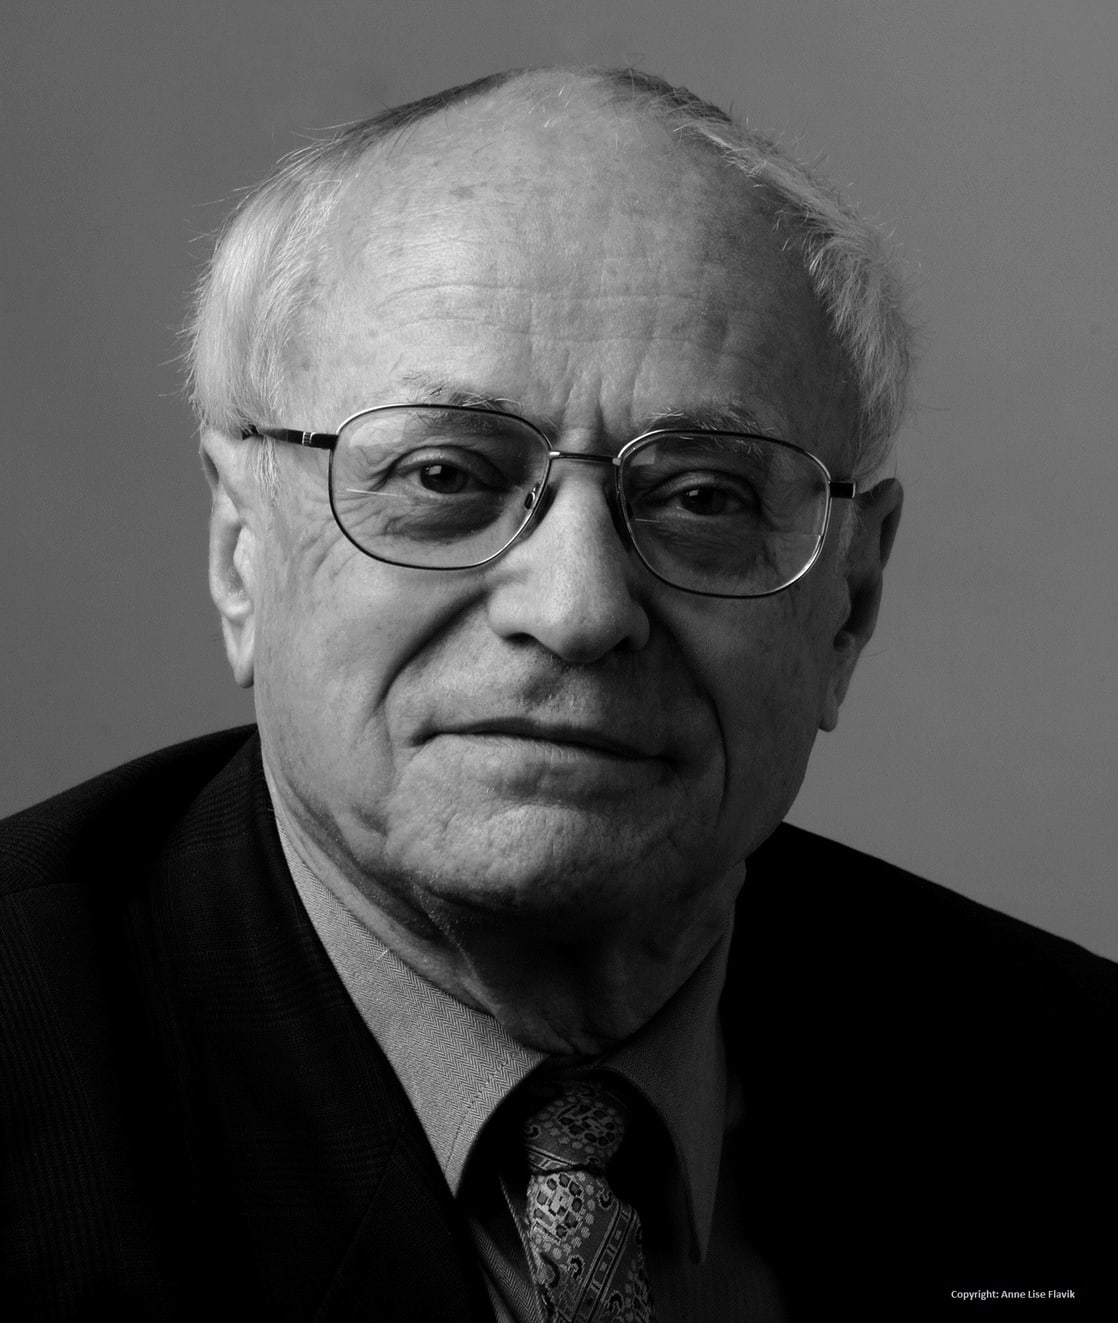
\includegraphics[scale=0.8]{images/serre}
\caption{Jean-Pierre Serre.}
\end{center}
\end{figure}

\begin{remark}
	A paper by Serre\footnote{``G\'eom\'etrie alg\'ebrique et g\'eom\'etrie analytique'' (GAGA), 1956.} says, roughly, that analytic maps over projective manifolds tend to be algebraic whereas analytic things over affine manifolds are much more common than algebraic things.
\end{remark}


\begin{example}[An automorphism of the affine plane]\label{}\text{}
Consider the endomorphism $\mathbf{A}^2\longrightarrow \mathbf{A}^2$ given by
\begin{align*}
	(x,y)\longmapsto  (x,xy).
\end{align*}
The image is not open, closed, or even locally closed. A theorem of Chevalley says that it must be a constructible set.\footnote{See EGA IV Th\'eor\`eme 1.8.4 (?).} For projective manifolds, the image of a closed set is closed.
\end{example}

\subsection{The Ax--Grothendieck theorem}
\begin{remark}
	[First-order logic]\index{first-order logic} In first-order logic, one uses the usual logical connectives $\land$, $\lor$, $\lnot$, $\implies$, etc. to make statements. Also, one can use the operations of the field or model in question. One may also quantify over all elements in the model $X$ (with ``for all $x\in X$, . . .'' or ``there exists $x\in X$, . . .'').

	Here's an attempt at saying, ``$\Omega$ is algebraically closed'':
	\begin{center}
		\small For all polynomials $a_nX^n + \cdots + a_1X + a_0\in \Omega[X]$, there is a root.
	\end{center}
	This is not allowed in first-order logic: One cannot say ``For all polynomials . . . .'' Here's the closest one can get:
	\begin{center}
		\small For all polynomials of degree $n$, there is a root.
	\end{center}
	This is allowed because it is a statement on $n$ coefficients in $\Omega$. To say that $\Omega$ is algebraically closed takes infinitely many statements in first-order logic. One cannot quantify over all integers.
\end{remark}
\begin{definition}[ ]\label{}\text{}
A theory is \defn{complete}\index{complete theory} if every statement in it is provable or disprovable.
\end{definition}

\begin{proposition}[ ]\label{}\text{}
The theory of algebraically closed fields of a given characteristic is complete.
\end{proposition}

\begin{proof}
There is a unique algebraically closed field of a given characteristic and cardinality $\mathfrak{c}$.
\end{proof}

\begin{remark}
	This means that anything true for all algebraically closed fields of large characteristic is true for algebraically closed fields of characteristic $0$. One cannot say that $\Omega$ is of characteristic $0$ with one statement in first-order logic. One needs a countably infinite number of statements: For every prime number $p$, the statement
	\begin{center}
		\small For all $\omega\in \Omega$, $p\omega\ne 0$.
	\end{center}
	must be true. Suppose you have proved something for algebraically closed fields of characteristic $0$. This proof uses only a finite number of axioms; that is, this proof can only eliminate a finite number of characteristics. Therefore, true for algebraically closed and characteristic $0$ implies true for algebraically closed and large characteristic.

	The converse is clearly true.
\end{remark}

\begin{theorem}[Ax--Grothendieck]\label{}\index{Ax--Grothendieck theorem}\text{}
Let $V$ be a variety over an algebraically closed field $k$. Let $f:V\longrightarrow V$ be a regular map. If $f$ is injective, $f$ is surjective.
\end{theorem}

\begin{example}[$k$ must be algebraically closed]\label{}\text{}
Consider $k= \mathbf{Q}$ and $f:\mathbf{A}^1\longrightarrow \mathbf{A}^1$ given by $f(x)=x^ 3$. This is injective but not surjective.
\end{example}

\begin{example}[The converse is false]\label{}\text{}
Let $k=\mathbf{C}$ and $f(x)=x^2$. This is surjective but not injective.
\end{example}

\begin{proof}
This is trivial if $k$ is finite. Also, this is true over any algebraic extension of a finite field: The coefficients of all equations defining a variety and those of a point lie in some finite field. It is true for algebraic closures of finite fields. Recall that a first-order statement is true for an algebraically closed field of characteristic zero if and only if it is true for algebraically closed fields of all sufficiently large characteristics. Also, if a first-order statement is true for one algebraically closed field of a given characteristic, it is true for all algebraically closed fields of that characteristic.
\end{proof}

\begin{remark}
	A well-known example of proving something for positive characteristics and extending it to characteristic $0$ is Mori's bend-and-break argument.
\end{remark}

\subsection{Rational maps}
Suppose $Y$ is an affine variety. The coordinate ring $\mathscr{O}(Y)$ is an integral domain. Hence, one can construct the field of fractions $K(Y)$. Its elements are called \defn{rational functions}\index{rational function} on $Y$.

\begin{example}[ ]\label{}\text{}
Suppose $Y=\mathbf{A}^2$. Then $\mathscr{O}(Y) = k[x,y]$ and $K(Y) =k(x,y)$. 
\end{example}

\begin{remark}
	Regular functions on affine varieties are analogous to holomorphic functions on Riemann surfaces; rational functions correspond to meromorphic functions.
\end{remark}

Now, suppose $Y$ is a projective variety. The previous construction does not work because the ring of regular functions $\mathscr{O}(Y)$ is just $k$ (whose field of fractions is itself). Instead, a rational function is given by the following:
 \begin{enumerate}
	\item A dense affine open set $U$;
	\item A rational function $f$ on $U$.
\end{enumerate}
One identifies $(f_1,U_1)$ and $(f_2,U_2)$ if $f_1=f_2$ on a dense open set containing $U_1$ and $U_2$. One gets the rational functions by taking a direct limit over dense open affine sets $U$ of the ring of regular functions on $U$. Therefore, the rational functions $K(Y)$ form a field.

\begin{remark}
	We are supposing that $Y$ is irreducible. One can define rational functions on a reducible algebraic set, but the rational functions do not form a field in that case.
\end{remark}

Suppose $X$ and $Y$ are varieties. A \defn{rational map}\index{rational map} $X\longrightarrow Y$ is a regular map $U\longrightarrow Y$ where $U$ is dense and open in $X$. One identifies $(f_1,U_1)$ and $(f_2,U_2)$ if $f_1=f_2$ on an open set contained in $U_1\cap U_2$.

\begin{example}[ ]\label{}\text{}
Rational maps $X\longrightarrow \mathbf{A}^1$ are rational functions on $X$.
\end{example}

Rational maps do not form a category: Composition does not need to be defined! For example, the composition of $0:\mathbf{A}^1\longrightarrow \mathbf{A}^1$ and $f:\mathbf{A}^1\longrightarrow \mathbf{A}^1$ given by $x\longmapsto 1/x$ is not defined.

\begin{definition}[ ]\label{}\text{}
A rational map is \defn{dominant}\index{dominant rational map} is a rational map whose image contains a dense open set.
\end{definition}

\begin{definition}
	Two varieties are \defn{birational}\index{birational equivalence} if they are equivalent in the category whose morphisms are dominant rational maps.
\end{definition}

\begin{remark}
	Birational equivalence is a cruder notion of equivalence than isomorphism.
\end{remark}

\begin{example}[ ]\label{}\text{}
Consider $\mathbf{A}^1$, $\mathbf{P}^1 $, the hyperbola $xy=1$ in $\mathbf{A}^2$, and the curve $x^3=y^2$. All of these are birational, though no two are isomorphic.

The varieties $\mathbf{P}^1\times \mathbf{P}^1$, $\mathbf{P}^2$, $\mathbf{A}^2$, and $\mathbf{A}^2-\{(0,0)\}$ are birational but not isomorphic.
\end{example}

\begin{remark}
	A variety that is birational to an affine space is called a \defn{rational variety}\index{rational variety}.
\end{remark}

\begin{problem}
	Find a non-rational variety.
\end{problem}

\begin{example}[ ]\label{}\text{}
Consider the curve $x^3+y^3=1$. Let us show that this is not birational to $\mathbf{A}^1$, and, more generally, that there is no dominant rational map from $\mathbf{A}^1$ onto it. Suppose we have a dominant map from $\mathbf{A}^1$ to the curve (this is non-constant). This means we have rational functions $x$ and $y$ with $x(t)^3+y (t)^3 =1$. Clearing denominators, we have 
\begin{align*}
	f(t)^3+g (t)^3=h (t)^3
\end{align*}
where $f$, $g$, and $h$ are coprime polynomials. Factoring, we get
\begin{align*}
	(f(t)+g (t)) (f(t)+\omega g (t)) (f(t) + \omega^2g (t)) = h(t)^3.
\end{align*}
The ring $k[t]$ in which these polynomials live is a UFD. Therefore, each term must be a cube (up to units, but the units are constants which are cubes in an algebraically closed field). Write
\begin{align*}
	h_1 (t)^3 h_2(t)^3  h_3(t)^3 = h (t)^3.
\end{align*}
One can eliminate $f$ and $g$ from the three equations one gets and a linear relation between $h_1^3$, $h_2^3$, and $h_3^3$ emerges. Multiplying by constants, one gets another relation between polynomials in which the sum of the cubes of the first two is the cube of the third. 

This gives another equation of the form above. If $f$, $g$, and $h$ are not constants, then $h_1$, $h_2$, and $h_3$ have smaller degree. This is a contradiction.
\end{example}

\begin{remark}
	This works for exponent greater than or equal to $3$. The result is false for exponent $2$:
	\begin{align*}
		(1-t^2)^2 +  (2t^2)^2 =  (1+t^2)^2.
	\end{align*}
	This corresponds to the fact that $x^2+y^2=1$ is rational.
\end{remark}

\begin{remark}
	The variety $\mathbf{A}^1$ has genus $0$ and $x^3+y^3=1$ has genus $1$. We will prove that there is no non-constant map from something to something of higher genus.
\end{remark}

\subsection{Elliptic functions and cubic curves}
We shall use elliptic functions to show that some cubic curves in the plane are not birational to the affine line.

Recall that $\wp$ is elliptic, so $\wp(z+\lambda) = \wp(z)$ where $\lambda$ is a point in a lattice $\Lambda$. This doubly periodic function is not holomorphic; if such a function were holomorphic, it would be bounded in a fundamental domain, so bounded everywhere, hence constant by Liouville's theorem. 

How does one find elliptic functions? One way is to take a function $g$ and sum over the lattice:
\begin{align*}
	f(z) :=  \sum_{\lambda\in \Lambda}^{} g (z+\lambda).
\end{align*}
This does not converge for $g(z) = 1/z$. This converges well for $g(z) = 1/z^3$ and borderline for $g(z)=1/z^2$ (that is, it doesn't converge for $1/z^2$, but does for $1/z^{2+\epsilon}$). Hence, we define
 \begin{align*}
	\wp(z) :=  \frac{1}{z^2} + \sum_{\lambda\ne 0}^{} \frac{1}{(z-\lambda)^2} - \frac{1}{\lambda^2}.
\end{align*}
One shows that this is doubly periodic by looking at its first derivative and noticing that it is doubly periodic and showing that the constant up to which $\wp$ is doubly periodic is $0$.

Let's look at its Laurent expansion at $z=0$:
\begin{align*}
	\wp(z) = z^{-2} + 0 z + *z^2 + \cdots.
\end{align*}
Now, its derivative:
\begin{align*}
	\wp'(z) = -2z^{-3} + *z +\cdots.
\end{align*}
Square the derivative:
\begin{align*}
	(\wp'(z)) ^2 = 4z^{-6} + *z^{-2} + *z^0 + \cdots.
\end{align*}
Further,
\begin{align*}
	4(\wp(z)) ^3 = 4z^{-6} + *z^{-2} + \cdots.
\end{align*}
Hence,
\begin{align*}
	(\wp'(z)) ^2 = 4(\wp(z)) ^3 +  *\wp(z) + * + z.
\end{align*}
The first part is doubly periodic with no poles, and the whole thing vanishes at $z=0$. Therefore, one has
\begin{align*}
	(\wp'(z)) ^2 = 4(\wp(z)) ^3 - g_2 \wp(z) -  g_3.
\end{align*}

Why are these called elliptic functions? The arc length of an ellipse is given by 
\begin{align*}
	\int_{0}^{t} \frac{dx}{\sqrt{4x^3 - ax - b} }. 
\end{align*}
Such integrals are called elliptic integrals. Write
\begin{align*}
	\kappa(z) = -\int_{z}^{\infty} \frac{ds}{\sqrt{4s^3 -g_2s - g_3} }. 
\end{align*}
Extending $\kappa\inv$ to $\C$ gives $\wp$. The inverses of such functions are doubly periodic, so they were called elliptic functions.

Now, consider the curve $C:y^2 = 4x^3 - g_2x-g_3$. Put $y=\wp'(z)$ and $x=\wp(z)$, and one sees that $(x,y)$ is on this curve. Hence, one has a map $\mathbf{C}-\Lambda \longrightarrow C$ given by
\begin{align*}
	z\longmapsto (\wp'(z),\wp (z)).
\end{align*}
It's somewhat unfortunate that we have to ignore the lattice, so we can define a map $f$ from $\mathbf{C}$ to the projective curve given by $C$ where $f(\Lambda) = \{\infty\}$. 

We have a doubly periodic function on our hands, so we have a map from $\mathbf{C}/\Lambda$ to the projective curve. (This is a homeomorphism of topological spaces.) One notices that $\mathbf{C}/\Lambda$ is isomorphic to $S^1\times S^1$ as a topological space, so it is a torus.

Any rational curve is the same as $\mathbf{P}^1$ up to a finite number of points. The variety $\mathbf{P}^1$ is isomorphic to $S^2$ and the curve $C$ is isomorphic to the torus $S^1\times S^1$. Therefore, the two are not birational.

\begin{remark}
	We constructed a doubly periodic function by taking (essentially) $\sum_{}^{} 1/(z-\lambda)^2 $. One can also do this for (singly) periodic functions by taking the almost-convergent $\sum_{}^{} 1/(z-\lambda)$ and reordering by absolute value. This is $\pi\cot (\pi z)$. Taking the logarithmic derivative gives the product formula of $\sin$.
\end{remark}

\subsection{Rationality of cubic surfaces}
We have seen that cubic curves such as $x^3+y^3+z^3=0$ in $\mathbf{P}^2$ are not rational. Now, look at a cubic suface $w^3+x^3+y^3+z^3= 0$ in $\mathbf{P}^3$. One might argue that setting $w=0$ gives a cubic curve in $\mathbf{P}^2$ that isn't rational, but this doesn't work. In fact, it is rational.

First, observe that it contains two not intersecting lines: $w+x=0, y+z=0$ and $w+y=0, x+\omega z=0$ where $\omega$ is a primitive cube root of unity. Pick one point on each line and connect them. The resulting line should intersect the surface at one other point (ignoring the possibility that it lies on the cubic surface). Therefore, we have sort of constructed a map from $\mathbf{P}^1\times \mathbf{P}^1$ to the cubic surface. This is a rational map that is not defined everywhere. One can conclude that this map is almost surjective. Does it have a rational inverse?

Suppose there is a point on the third line that another line that goes through the first two lines intersects. This is a contradiction, since we assumed that the first two lines were skew. Hence, it is injective and (with some work) has a rational inverse; this strongly suggests that it's birational to $ \mathbf{P}^1\times \mathbf{P}^1$, and it is. Therefore, if a cubic surface has two not intersecting lines, it is birational to $\mathbf{P}^1\times \mathbf{P}^1$. Let's look at a different argument.

Pick $6$ points in $\mathbf{P}^2$ in general position (in this case, no three points are on a line and not all are on a conic). The space of cubic functions in three variables is $10$ dimensional. Consider the cubics that vanish on all $6$ points. This gives a $4$ dimensional space. Suppose this is spanned by $f_1$, $f_2$, $f_3$, and $f_4$.

Try to define a map $\mathbf{P}^2 \longrightarrow \mathbf{P}^3$ by 
\begin{align*}
	(x:y:z)\longmapsto  (f_1:f_2:f_3:f_4).
\end{align*}
However, this is not defined at the $6$ points. So this is a rational map, not a regular map. What is its image?

One guesses that it's a hypersurface, so assume so. What is the degree of this hypersurface? Pick a line in $\mathbf{P}^3$, say $f_1=f_2=0$. Both $f_1$ and $f_2$ are cubics, so \index{B\'ezout's theorem}B\'ezout's theorem says that they have $9$ points of intersection. Six of these are the points with which we started, which leaves $3$ points. Therefore, the hypersurface has degree $168$ (just kidding: it has degree $3$).

The dimension of the space of cubics in $\mathbf{P}^3$ has dimension $20$. Therefore, the dimension of the space of cubic surfaces is $19$.  (Think of each cubic surface as being a point in a parameter space. This parameter space is $\mathbf{P}^{19}$.) 

The dimension of the parameter space of the six points is $6\cdot 2$. Further, $\dim (\Aut(\mathbf{P}^2))=8$ and $\dim(\Aut(\mathbf{P}^3)) =15$. The dimension of the space of cubic surfaces one gets by taking $6$ points in $\mathbf{P}^2$ is probably going to be $12+15-8=19$, which strongly suggests that one can get all nonsingular cubic surfaces from this construction. Dr. Borcherds states about this argument:
\begin{center}
	\small It's got more holes in [it] than a piece of Swiss cheese.
\end{center}

These kinds of arguments were typical of old school algebraic geometry. Proving this true claim takes a lot more work.

\begin{problem}
	How might one guess that there are $27$ lines on a cubic surface from this construction?
\end{problem}

Take $6$ points in $\mathbf{P}^2$ as before. The map above is indeterminate at these points, and there are lines on the cubic surface whose preimages are these points. That is, $6$ points give rise to $6$ lines on the cubic. One also gets $15$ lines in $\mathbf{P}^2$ through $2$ of the $6$ points whose images are lines on the cubic surface. Lastly, take a conic through five of the points. There are $6$ conics through $5$ points, and the image of each is a line on the cubic surface. Altogether, there are $27$ lines.

\subsection{Blowing up a point}
\index{blowing up} 
\begin{example}[ ]\label{}\text{}
Take the curve $y^2 = x^3 +x^2$. This has a singularity at $(0,0)$. Let $y=tx$. Then one has $t^2x^2 = x^3+x^2$, which factorizes as follows:
\begin{align*}
x^2(t^2 - (x+1)) =0.
\end{align*}
One gets $2$ curves in the $(x,t)$ plane: $t^2=x+1$ and $x=0$. We get rid of the singularity but pick up another curve. The curve $x=0$ is called the \defn{exceptional curve}\index{exceptional curve}. This is blowing up.
\end{example}


Suppose we want to blow up the $(x,y)$ plane $\mathbf{A}^2$ at $(0,0)$. We introduce two new variables $(X:Y)\in  \mathbf{P}^1$. Consider the points $((x,y),  (X:Y))$ in $\mathbf{A}^2\times \mathbf{P}^1$ such that 
\begin{align*}
	xY = Xy.
\end{align*}
If $(x,y)\ne (0,0)$, there is one point of $\mathbf{P}^1$ to which it corresponds. If $(x,y)= (0,0)$, any point in $\mathbf{P}^1$ satisfies this. This subset of $\mathbf{A}^2\times \mathbf{P}^1$ is called the \index{blow up}blow up of $\mathbf{A}^2$ at a point (this is a \index{quasiprojective variety}quasiprojective variety). We get a map from the blow up to $\mathbf{A}^2$ given by
\begin{align*}
	((x,y), (X:Y)) \longmapsto (x,y).
\end{align*}
The preimage of a nonzero point in $\mathbf{A}^2$ is one point and that of $(0,0)$ is $\mathbf{P}^1$. The projective line $\mathbf{P}^1$ is covered by two affine lines: $X = 1$ and $Y=1$. If $X=1$, then we have the transformation $xY=y$, and, if $Y=1$, we have $x = Xy$.

This generalizes. Take $\mathbf{A}^n$ with coordinates $(x_1,\hdots, x_n)$ and $\mathbf{P}^{n-1}$ with coordinates $(X_1:\cdots : X_n)$. Consider the subvariety of $\mathbf{A}^n\times \mathbf{P}^{n-1}$ given by the relation $x_iX_j = x_jX_i$ for all $i$ and $j$. This maps onto $\mathbf{A}^n$. The inverse image of $(x_1,\hdots, x_n)$ is a point if it's not $(0,\hdots, 0)$ and $\mathbf{P}^{n-1}$ if it is. The space $\mathbf{P}^{n-1}$ is covered by affine subsets of the form $X_i=1$, so we get $X_j = x_j/x_i$. That is, the effect of blowing up on the subset $X_i$ is introducing new coordinates by dividing the original coordinates by $x_i$.

\begin{example}[Resolving a singularity]\label{ressing}\text{}
We haven't formally defined \index{singularity}singularities yet, but they're fairly straightforward to understand. The curve $y^2=x^3$ has a singular point at $(0,0)$. Let us blow up at $(0,0)$. Let $y=xt$, so 
\begin{align*}
	x^2(t^2-x)=0.
\end{align*}
In the $(x,t)$ plane, one has the exceptional curve $x=0$ and the curve $t^2=x$. These curves have no singular points.
\end{example}

\begin{example}[ ]\label{}\text{}
Consider the surface $x^2+y^2=z^2$ (a cone). There is a singularity at $(0,0,0)$. Let us blow up at $(0,0,0)$. Choose to divide by $z$, so $y=zs$ and $x=zt$. One gets
\begin{align*}
	z^2(t^2+s^2-1)=0.
\end{align*}
In the $(z,s,t)$ plane, the surface in question transforms into a cylinder given by $t^2+s^2-1$ and the exceptional plane $z=0$. The singularity has been resolved.
\end{example}

\begin{example}[ ]\label{}\text{}
Consider $y^8=z^5$. Blow this up once: If one divides $y$ by $z$, let $z=yt$. Then
\begin{align*}
	y^5(t^5-y^3)=0.
\end{align*}
The curve $y=0$ is exceptional, and $t^5-y^3$ still has a singularity, so blow it up again. Let $y= ts$. Therefore,
\begin{align*}
	t^3(s^3-t^2)=0.
\end{align*}
The curve $t=0$ is exceptional, and one blows up $s^3=t^2 $ by letting $t=su$, which means that $s=0$ and $s=u^2$ (see \cref{ressing}). Finally, the singularity has been resolved. 
\end{example}

\begin{example}[Pinch point\index{pinch point}]\label{ppoint}\text{}
Consider $xy^2=z^2$. (This is called the \defn{Whitney umbrella}\index{Whitney umbrella}.) The points on the $x$ axis are the only singular points. The point $(0,0,0)$ seems to be worse off than the rest of them, so we blow it up. Take the variety $\mathbf{A}^3 \times \mathbf{P}^2$ with coordinates $((x,y,z),  (X:Y:Z))$. Choose one of the projective coordinates to be $0$ such that one of the affine pieces covers it. Dividing by $x$, we let $y=xY$ and $z=xZ$. Then, we get
\begin{align*}
	x^2(xY^2-Z^2)=0.
\end{align*}
Hence, we have transformed the singularity into an exceptional curve and another singularity. Notice that the new singularity is the same as the one with which we started. Oh no. Well, we can blow up a line, not just a point.

Take coordinates $(x,y,z)$, and, instead of taking $\mathbf{P}^2$, take $\mathbf{P}^1$ with coordinates $(s:t)$. Assert $yt=zs$. We have $xy^2=z^2$, so if we blow up along this line, we should choose $s=1$ or $t=1$. Choose $s=1$. Then $yt=z$. Thus, $y^2=0$ or $x=t^2$.
\end{example}

\begin{warn}
	One needs to define ``worst singularity'' in a very precise manner, as corroborated in \cref{ppoint}. 
\end{warn}

\subsection{More on blow ups}
\begin{example}[Blowing up a point of $\R^2$]\label{}\text{}
Blow up $(0,0)\in  \mathbf{R}^2$. Consider the coordinates $(x,y)$, and introduce new coordinates $(s:t) \in \mathbf{P}^1$. Take the set of points $((x,y), (s:t)) \in \mathbf{R}^2\times \mathbf{P}^1$ such that $xt=ys$. Every nonzero point in $\mathbf{R}^2$ corresponds to a unique point of the blow up and the zero point of $\mathbf{R}^2$ blows up to $\mathbf{P}^1(\mathbf{R})\isomto S^1$  (one can think of this having a point for every possible direction through the point). Hence, we have a map from the blow up to $\mathbf{P}^1(\mathbf{R})$ given by
\begin{align*}
	((x,y),  (s:t)) \longmapsto (s:t).
\end{align*}
The preimage of a point $(s:t) \in \mathbf{P}^1$ is a copy of $\mathbf{R}$. Let $E$ be the blow up. Then one has a map $E\longrightarrow S^1$ whose fibres are $\mathbf{R}$. One might guess that this might be a cylinder, but that's not right: The blow up is non-orientable\index{non-orientable surface}. Therefore, it is homeomorphic to an open M\"obius strip. 
\end{example}

\begin{example}[ ]\label{}\text{}
Let us construct a map 
\begin{align*}
	\mathbf{P}^1\times \mathbf{P}^1\longrightarrow \mathbf{P}^2.
\end{align*}
One might try with $((x_0:x_1),(y_0:y_1)) \longmapsto (x_0y_0:x_1y_0:x_0y_1)$. This is not defined if $x_0=y_0=0$, but we can make it so by blowing up $\mathbf{P}^1\times \mathbf{P}^1$ at $((0:1), (0:1) )$. Cover it with a copy of $\mathbf{A}^2$ with coordinates $(x_0,y_0)$ given by the points $x_1=1,y_1=1$. One blows up at $(0,0)$ and finds there is a map from this blown up plane to $\mathbf{P}^2$: Write $x_0=ty_0$, so $(x_0y_0:x_1y_0:x_0y_1)$ becomes $(ty_0^2:x_1y_0:ty_0y_1)$ or $(ty_0:x_1:ty_1)$. This is a good point of $\mathbf{P}^2$.

Therefore, one gets a regular map from the blow up of $\mathbf{P}^1\times \mathbf{P}^1$ to $\mathbf{P}^2$ from a rational map $\mathbf{P}^1\times \mathbf{P}^1\longrightarrow \mathbf{P}^2$.

\begin{remark}
	This regular map is not an isomorphism. The point $(0:0:1)\in  \mathbf{P}^2$ is the image of the line $y_0=0$ in $\mathbf{P}^1\times \mathbf{P}^1$ and $(0:1:0)\in \mathbf{P}^2$ is the image of the line $x_0=0$. This map is just the map one gets by blowing up these two points of $\mathbf{P}^2$. That is, the blow up of $\mathbf{P}^1\times \mathbf{P}^1$ at one point is the blow up of $\mathbf{P}^2$ at two points.
\end{remark}
\end{example}

The geometric meaning of blowing up a point is taking it to the projective space over its tangent space. We have seen that we can blow up a line, and, more generally, we can blow up a subvariety $X$; the geometric interpretation here is mapping a point in $X$ to the projective space over the normal space at that point. 

We can also blow up an ideal or a \index{quasicoherent sheaf}quasicoherent sheaf of graded algebras. One can construct a projective variety from a graded algebra. Suppose we have a graded algebra for every point in the variety and replace every point by the projective space of the corresponding graded algebra. That's a blow up. But how does one assign a graded algebra to every point of the variety? The nice way to do this is through a quasicoherent sheaf of graded algebras. (More on that in the next chapter.) This corresponds to the projective space of a graded algebra at each point.

There is one straightforward example to consider: Suppose the variety is a point. Then a quasicoherent sheaf of graded algebras is a graded algebra, say $k[x_0,\hdots,x_n]$. Blowing up a point along this sheaf is the usual construction of $\mathbf{P}^n$.

\begin{example}[ ]\label{introsing}\text{}
Consider the affine plane $\mathbf{A}^2$ with coordinate ring $k[x,y]$. Blowing up a point $(0,0)\in  \mathbf{A}^2$ corresponds to blowing up the ideal $(x,y)$. Suppose $g_1,\hdots, g_n\in k[x,y]$ generate an ideal. Take the set of all pairs $((x,y), (g_1:\cdots:g_n))$ in $\mathbf{A}^2\times \mathbf{P}^{n-1}$ where $x$ and $y$ are not in the subvariety generated by the $g_i$. Take the closure of the image of $\mathbf{A}^2- V$ in $\mathbf{A}^2\times \mathbf{P}^{n-1}$.

Take $I=(x^2,y^2)$. Then, take 
\begin{align*}
	(x,y)\longmapsto  ((x,y), (x^2:y^2)) \in \mathbf{A}^2\times \mathbf{P}^1.
\end{align*}
Write the elements in the image $((x,y),  (s:t))$. The projective line is covered by two copies of the affine line. Take $s=1$. Notice that $x^2t = y^2s$ so $x^2t=y^2$. This is the Whitney umbrella\index{Whitney umbrella}.
\end{example}

\begin{warn}
	One must be careful about blowing up. While Hironaka showed that blowing up always resolves singularities in characteristic $0$, if you blow up the wrong thing, you may introduce new singularities, as was demonstrated at the end of \cref{introsing}.
\end{warn}

\subsection{The Atiyah flop}
\begin{figure}
\begin{center}
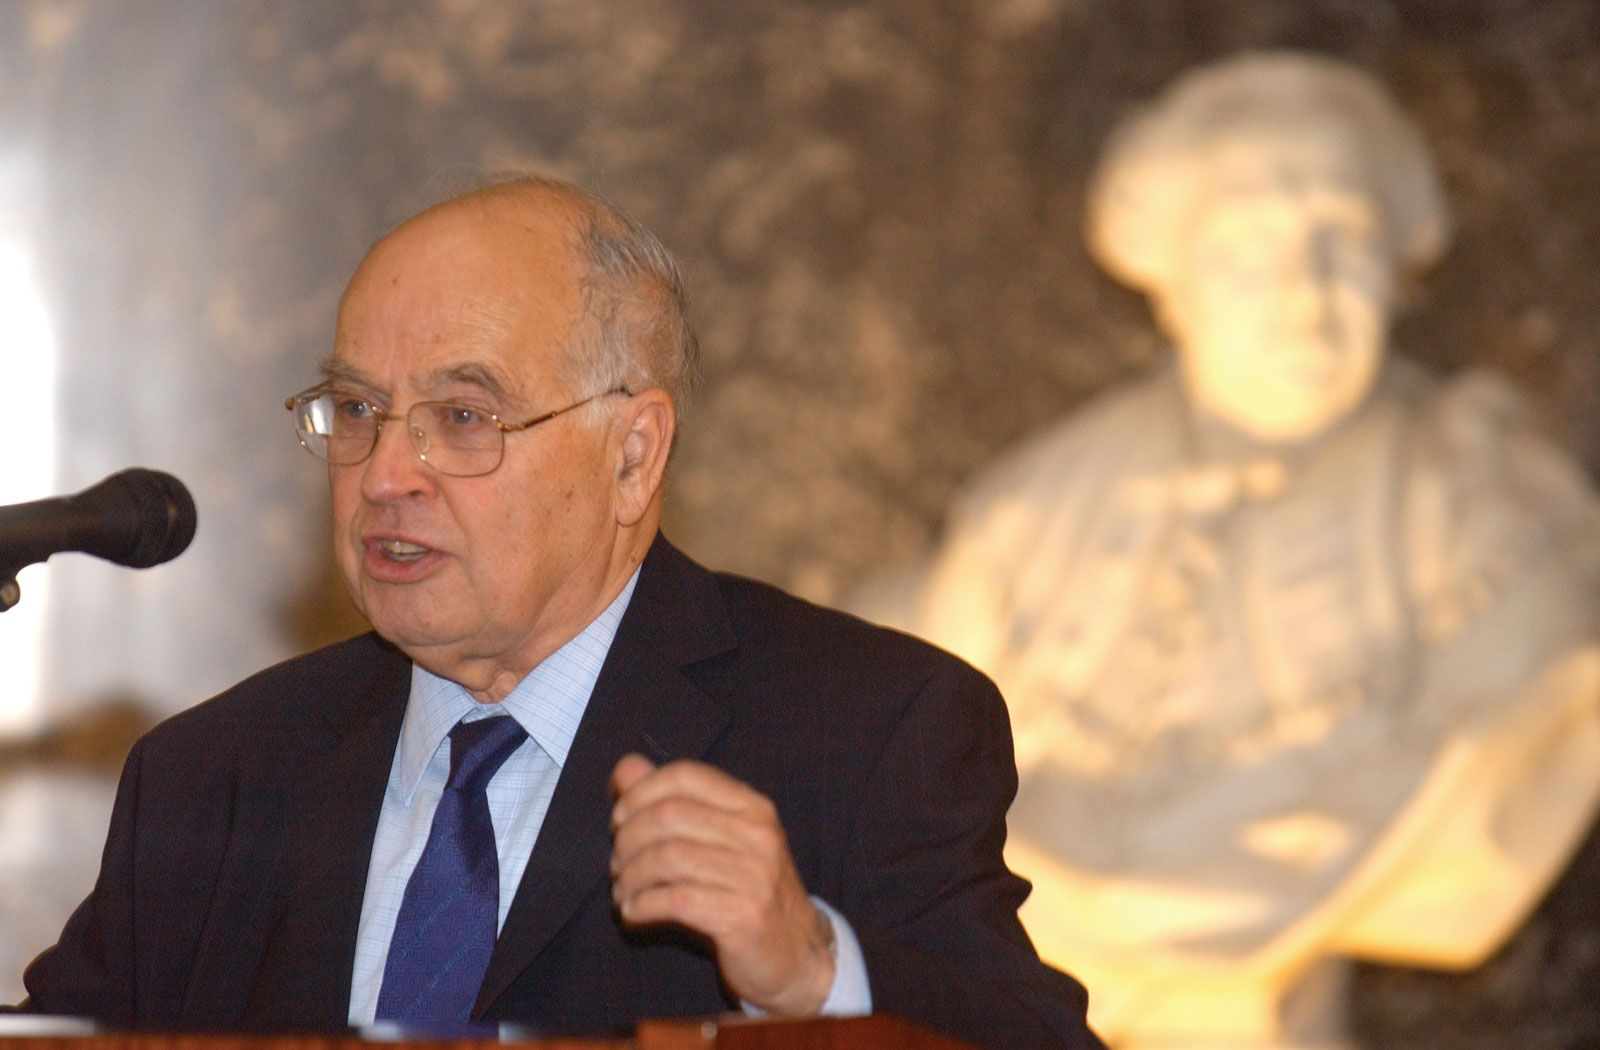
\includegraphics[scale=0.15]{images/atiyah}
\caption{Michael Atiyah.}
\end{center}
\end{figure}
Consider the hypersurface $xy=zt$ in $\mathbf{A}^4$. This looks like a cone over $\mathbf{P}^1\times \mathbf{P}^1$: One looks at the corresponding variety of points $(x:y:z:t)\in \mathbf{P}^3$ satisfying $xy=zt$. This is a quadric in projective space, which gives a product $\mathbf{P}^1\times \mathbf{P}^1$ (cf. \cref{seg}). In particular, this variety has a singularity at $(0,0,0,0)$ that is the singular point of the cone.

One resolves this singularity by blowing up at $(0,0,0,0)$. Consider points $((x,y,z,t),  (X:Y:Z:T)) \in \mathbf{A}^4\times \mathbf{P}^3$ satisfying $xy=zt$, $xY=Xy$, $xZ = Xz$, etc. Take the image of the nonzero points in $\mathbf{A}^4$ under
\[
	(x,y,z,t)\longmapsto  ((x,y,z,t),  (X:Y:Z:T))
	\]
	Taking the Zariski closure of the image, one also has the equation $XY=ZT$. Every nonzero point of $\mathbf{A}^4$ corresponds to a unique point in the blow up $\mathbf{A}^4\times \mathbf{P}^3$ while $(0,0,0,0)$ corresponds to a copy of $\mathbf{P}^1\times \mathbf{P}^1$. This is not singular\iffalse, since, along $X=1$, it becomes $Y=ZT$ in the coordinates $(x,Y,Z,T)$\fi.

	One can also resolve this by blowing up to $\mathbf{P}^1$: Blow up along the line $y=t=0$. Consider the points $((x,y,z,t),  (X:Z)) \in \mathbf{A}^4\times \mathbf{P}^1$. Blowing up, we get the equations $xy=zt$ and $xZ=Xz$. However, taking the closure of the image of $\mathbf{A}^4$, we get the equation $tZ = Xy$, too. Say $X=1$. Then $y=tZ$, $z=xZ$, and $xy=tz$, which reduces to affine $3$-space. Hence, the blow up non-singular. The point $(0,0,0,0)$ is blown up to $\mathbf{P}^1$. (One can also blow up along $x=z=0$, which results in a distinct resolution to $\mathbf{P}^1$.)

	The birational map from the first resolution to the second resolution is called the \defn{Atiyah flop}\index{Atiyah flop}.\footnote{This explanation from Wikipedia is slightly more clear: Let $Y$ be the zeros of $xy=zw$ in $\mathbf{A}^4$, and let $V$ be the blowup of $Y$ at the origin. The exceptional locus of this blowup is isomorphic to $\mathbf{P}^1\times \mathbf{P}^1$ and can be blown down to $\mathbf{P}^1$ in two different ways, giving varieties $X_1$ and $X_2$. The natural birational map from $X_1$ to $X_2$ is the Atiyah flop.}
	\begin{figure} 
		\begin{center}
			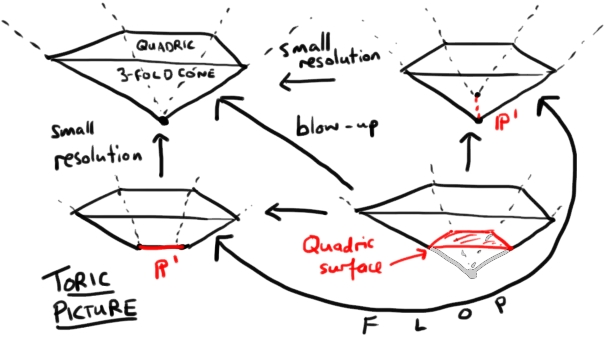
\includegraphics[scale=0.53]{images/flop_1}
			\caption{An illustration of a flop.}
		\end{center}
	\end{figure}

	\begin{figure}
		\begin{center}
			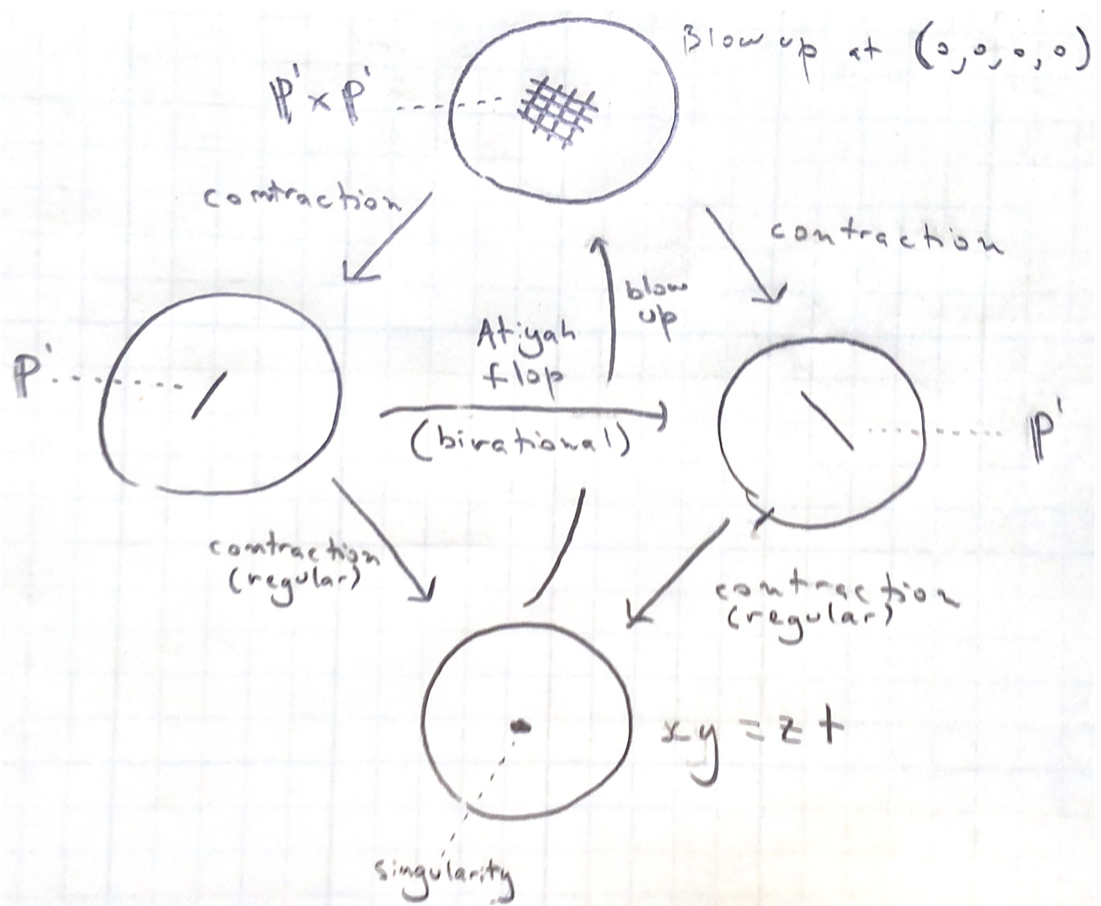
\includegraphics[scale=0.53]{images/atiyah_flop}
			\caption{An illustration of the Atiyah flop.}
		\end{center}
	\end{figure}

	This shows that there is no minimal way to resolve singularities in general. If one wants to find a minimal model---a ``smallest possible'' resolution of singularities---the best thing to do is to allow ``mild'' singularities in it. (More precisely, one allows \index{terminal singularity}terminal singularities.)

\subsection{Singular points}
Suppose $p$ is a point of a variety $V$. The point $p$ is called \defn{singular}\index{singular point} if the tangent space at $p$ has the wrong dimension (that is, the dimension is greater than the dimension of $V$).

Let $p=(0,\hdots, 0)\in  \mathbf{A}^n$ and $V$ the set of points at which an irreducible polynomial $f$ vanishes. Then the \defn{tangent space}\index{tangent space} at $p$ is given by the roots of the linear part of $f$. For example, if this irreducible polynomial is $x-2y-3x^2+4xy =0$, the tangent space is given by $x-2y=0$.

Let $f(x,y)=0$ be a plane curve. Saying that $(0,0)$ is singular is equivalent to saying that $f(0,0)=0$ and the linear terms vanish. If the linear terms vanish, the tangent space is $\mathbf{A}^2$, which is the wrong dimension.

\begin{example}[ ]\label{}\text{}
For the curves $y^2 = x^3$ and $y^2 = x^3+x^2$, the tangent spaces at $(0,0)$ are two dimensional.
\end{example}

If one has $f(x_1,\hdots, x_n) =0$, then saying that $(0,\hdots, 0)$ is singular is equivalent to saying that $f(0,\hdots,0)=0$ and the linear terms vanish: 
\begin{align*}
	\frac{\partial f}{\partial x_i}(0,\hdots, 0) =0.
\end{align*}

Suppose $V\subseteq \mathbf{A}^n$ is the zero set of polynomials $f_1,\hdots$. Take $p=(0,\hdots, 0)$, so all $f_i$ vanish at $p$. The tangent space is the common roots of all linear parts of $f_1,\hdots$. The dimension of the tangent space is given by the rank of the Jacobian:
\begin{align*}
	\dim(\textrm{tangent space at $p$}) = n-\rank \frac{\partial f_i}{\partial x_j}.
\end{align*}
This is difficult to compute in general, which is why we started with codimension-$1$ hypersurfaces. However, one sees that the subset of singular points is closed: the condition for a matrix having rank less than a fixed constant is a closed condition on the entries. Therefore, the condition for the tangent space having the wrong dimension is closed.

\begin{warn}
	For varieties, the set of singular points is closed, but this does not hold for schemes.
\end{warn}

\begin{proposition}[ ]\label{}\text{}
The nonsingular points of a variety are dense.
\end{proposition}

The nonsingular points comprise an open set, so one needs to show that the set of nonsingular points is nonempty. 

\begin{example}[ ]\label{}\text{}
Consider the variety $x^3+y^3=1$. Over $\mathbf{C}$, there are no singular points. However, over a field of characteristic $3$, all points are singular. What goes wrong: $x^3+y^3-1=(x+y-1)^3$ is not irreducible over $\mathbf{F}_{3}$.
\end{example}


First, we reduce to the case of hypersurfaces. The key is that every variety $V$ is birational to a hypersurface. Consider the function field $K$ of the variety $V$. Choose $x_1,\hdots, x_n$ such that $K$ is separable over $k(x_1,\hdots, x_n)$. Then it is generated by $1$ element, so $K=k(x_1,\hdots, x_n,y)$ and $f(x_1,\hdots, x_n,y)=0$ for some $f$.

Consider the hypersurface $f(x_1,\hdots, x_n)=0$ where $f$ is irreducible. Also, suppose that the field $k$ over which we are working is algebraically closed. If all points are singular, then 
\begin{align*}
	\frac{\partial f}{\partial x_i} =0
\end{align*}
at all points of $V$. But $\deg \partial f/\partial x_i< \deg f$, and, since $f$ is irreducible, $f\mid \partial f/\partial x_i$, so $\partial f/\partial x_i =0$. This implies that $f=0$ in characteristic $0$ and that $f$ is a linear combination of $p$th powers of monomials in characteristic $p$. This implies that $f=g^p$, so $f=0$  (since $k$ is algebraically closed).

 \begin{remark}\label{convvv}
	At nonsingular points over $\mathbf{R}$ or $\mathbf{C}$, a variety $V$ looks like a smooth manifold locally.
\end{remark}

\begin{example}[The converse of \cref{convvv}]\label{}\text{}
Consider $y^2=x^3$ over $\mathbf{R}$. This is a topological manifold.
\end{example}

\subsection{The Zariski tangent space}
We would like to determine a definition of ``tangent space'' that does not depend on how one embeds the variety $V$ into affine space.

 \begin{definition}[ ]\label{}\text{}
The \index{tangent space}tangent space at a point is the dual of the \index{cotangent space}cotangent space at that point.
\end{definition}

\begin{remark}
	From the perspective of differential geometry, this definition seems circular. However, while the tangent space is fundamental in differential geometry, the cotangent space is fundamental in algebraic geometry.
\end{remark}

One defines the cotangent space as $\mathfrak{m}/\mathfrak{m}^2$ where $\mathfrak{m}$ is the maximal ideal of the local ring\index{local ring} at the point---the ring of functions of the form $f/g$ where $g\ne 0$ there. Hence, one might think of $\mathfrak{m}$ as functions vanishing at the point. The local ring at a point does not depend on the embedding of the variety as desired, but is this definition the same as the earlier one?

Consider $p= (0,\hdots, 0)$ for simplicity and $V\subseteq \mathbf{A}^n$ with coordinates $(x_1,\hdots, x_n)$. The maximal ideal $\mathfrak{m}$ is generated by $x_1,\hdots,x_n$, so $V$ is the set of zeros of functions $f_1,\hdots, f_n$. Now $\mathfrak{m}$ is $(x_1,\hdots, x_n)$ modulo $(f_1,\hdots, f_n)$ and all monomials of degree greater than or equal to $2$. This is the vector space spanned by $x_1,\hdots, x_n$ modulo the linear parts of the $f_i$s. This is the dual of the tangent space. Therefore, the new definition is compatible with the old one.

\begin{remark}
	This definition works for any local ring $R$: The quotient $\mathfrak{m}/\mathfrak{m}^2$ is a vector space over $R/\mathfrak{m}$. The space $\mathfrak{m}/\mathfrak{m}^2$ is called the \defn{Zariski cotangent space}\index{Zariski cotangent space} of the local ring. The \defn{Zariski tangent space}\index{Zariski tangent space}, naturally, is the dual of this.
\end{remark}

\begin{figure}
\begin{center}
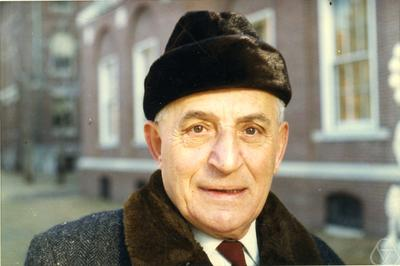
\includegraphics[scale=0.8]{images/zariski}
\caption{Oscar Zariski.}
\end{center}
\end{figure}


Let $R$ be a local ring. The quotient $\mathfrak{m}/\mathfrak{m}^2$ is an $R/\mathfrak{m}$--vector space whose dual $(\mathfrak{m}/\mathfrak{m}^2) ^*$ can be seen as ring homomorphisms 
\begin{align*}
	R\longrightarrow k[\epsilon]/(\epsilon^2).
\end{align*}
The target here is a two-dimensional vector space with a basis $\{1,\epsilon\}$ and $\epsilon^2=0$. This takes $\mathfrak{m}^2$ to $(0)$ and $\mathfrak{m}$ to multiples of $\epsilon$. A ring $k[x_1,\hdots, x_n]/I$ often corresponds to a variety or algebraic set. However, this only works if $I$ is reduced (has no nilpotents), and $\epsilon$ is nilpotent. 

It actually corresponds to the scheme $\Spec k[\epsilon]/(\epsilon^2)$. The only prime ideal of $k[\epsilon]/(\epsilon^2)$ is $(\epsilon^2)$, so one might say its spectrum looks like a point; however, it is better thought of as a point with a tangent vector corresponding to the point $\epsilon$.

Consider vector fields on a smooth manifold $V$ over $\mathbf{R}$. Look at the ring of smooth functions $C(V)$. The space of vector fields is a $C(V)$-module. Define the module $W$ of cotangent vector fields to be the dual of the module of vector fields. Recall, from differential geometry, that there is a map
\begin{align*}
	d:C(V) \longrightarrow W
\end{align*}
where $f$ maps to its $1$-form. Note that $d$ is not linear; it satisfies Leibniz's rule. 

Instead of considering $C(V)$, we might consider $R=k[x_1,\hdots, x_n]/I$.\footnote{See \url{https://en.wikipedia.org/wiki/Kähler_differential}.} We want to find a map $d$ from $R$ to an $R$-module $W$ that one thinks of as the module of cotangent vectors.

Note that $W$ is generated over $R$ by elements $dr$ for $r\in R$. One asserts $dr=0$ for $r\in k$ and Leibniz's rule. Define $W$ to be the module with these generators and relations.

\begin{example}[ ]\label{}\text{}
Take $R=k[x_1,\hdots, x_n]$. Then $W$ is the free module on $dx_1,\hdots, dx_n$. One defines the module of tangent vector fields by $\Hom_{R}(W, R)$.
\end{example}

\begin{remark}
	The module $W$ is free only when the cotangent bundle is a sum of trivial bundles. Otherwise, $W$ is quite hard to compute.
\end{remark}

Consider the homomorphism $R\tensor R\longrightarrow R$.\footnote{For now, $\tensor=\tensor_k$.} Let $\mathfrak{h}$ be the kernel of this homomorphism. Write $W = \mathfrak{h}/\mathfrak{h}^2$. (Note that $\mathfrak{h}$ is an ideal of $R\tensor R$.) Define 
\begin{align*}
	d :R\longrightarrow W
\end{align*}
by $dr = 1\tensor r - r\tensor 1$. The set $W$ is an $R$-module: $R$ acts by multiplication on the left $R$ in $R\tensor R$. Leibniz's rule holds. However, one needs to check the universal property.

That is, suppose there is an $R$-module $M$ with a map $d:R\longrightarrow M$ satisfying Leibniz's rule and a map from $R$ to $W$. One wants to show that there is a unique map such that
\begin{center}
	\begin{tikzcd}
		R \ar[r, "d"] \ar[dr, swap, "d"]&M\\&W\ar[u,dashed]
	\end{tikzcd}
\end{center}
commutes. One has $\mathfrak{h}\subseteq R\tensor R\longrightarrow R$, a map $R\longrightarrow \mathfrak{h}$, and a map $d:R\longrightarrow M$. One can define $f:R\tensor R\longrightarrow M$ by $a\tensor b \longmapsto a(db)$. This gives a map $f:\mathfrak{h}\longrightarrow M$. However, we want a map from $\mathfrak{h}/\mathfrak{h}^2$ to $M$, so we check that $f$ is $0$ on $\mathfrak{h}^2$.

Pick $\sum_{i}^{} s_i\tensor t_i\in \mathfrak{h}$ and $\sum_{j}^{} u_j\tensor v_j\in \mathfrak{h}$. So $\sum_{i}^{} s_it_i=0$ and $\sum_{j}^{} u_jv_j=0$. Now
\begin{align*}
	f \left( \left( \sum_{i}^{} s_i\tensor t_i \right)\tensor \left( \sum_{j}^{} u_j\tensor v_j \right)  \right)&= \sum_{i,\,j}^{} s_iu_j\, d(t_iv_j) \\
														   &= \left( \sum_{i}^{} s_i\, dt_i \right) \underbrace{\left( \sum_{j}^{} u_jv_j \right)}_{0} + \underbrace{\left( \sum_{i}^{} s_it_i \right)}_{0} \left( \sum_{j}^{} u_j\, dv_j \right) \\
														   &=0
\end{align*}
as desired.

From here, it is straightforward to show that $W$ is the universal module with a map $R\longrightarrow W$ satisfying Leibniz's rule.


\begin{remark}
	A local ring is \defn{regular}\index{regular local ring} if the dimension of the Zariski tangent space is the dimension of the local ring. A variety is nonsingular at a point if its local ring is regular.
\end{remark}

\subsection{Du Val singularities}
A \index{Du Val singularity}Du Val singularity may also be called a \index{simple surface singularity}simple surface singularity, a \index{Kleinian singularity}Kleinian singularity, a \index{rational double point}rational double point, or a \index{canonical singularity}canonical singularity in dimension $2$.

Take a finite group $G$ acting on $\mathbf{C}^2$. Take $\mathbf{C}^2/G$. For reasonable groups $G$, this gives a variety that has a singular point at the origin. Recall that the quotient is the ring of invariants of the coordinate ring of $\C$ under $G$: $k[x,y]^G$. 

Suppose $G=\Zmod n$ is generated by $\sigma$. Suppose further that $\sigma x = \zeta x$ and $\sigma y =\zeta^{-1}y$ where $\zeta$ is a primitive $n$th root of unity. Invariants under this action are given by $X =x^n$, $Y=y^n$, and $Z=xy$. Hence, one has
\begin{align*}
	k[x,y]^G = k[X,Y,Z] / (Z^n- XY).
\end{align*}
The Du Val singularities are classified as follows:
\begin{enumerate}
	\item $\Ag_n$ (Cyclic singularities): $x^2+y^2+z^{n+1}=0$;
	\item $\D_n$ (Dihedral singularities): $x^2+zy^2+z^{n-1}=0$;
	\item $\E_6$ (Tetrahedral singularity): $x^2+y^3+z^4=0$;
	\item $\E_7$ (Octahedral singularity): $x^2+y^3+yz^3=0$;
	\item $\E_8$ (Icosahedral singularity): $x^2+y^3+z^5=0$.
\end{enumerate}
The icosahedral singularity is not given by the icosahedral group of order $60$ acting on $\mathbf{C}^2$. The binary icosahedral group of order $120$ acts on $\mathbf{C}^2$ and gives this. 
\begin{remark}
	For the remainder of this section, we work in characteristic $0$ and the only singular point is $(0,0,0)$.
\end{remark}
\begin{example}[Resolving the icosahedral singularity]\label{}\text{}
The idea is to blow up the singular point until we don't get a singular point back. Consider the variety $x^2+y^3+z^5=0$. Let us introduce coordinates in $\mathbf{P}^2$ given by $(x_1:y_1:z_1)$. Assert $xy_1=x_1y$, $xz_1=x_1z$, and $yz_1=y_1z$. The projective plane $\mathbf{P}^2$ is covered by $3$ copies of $\mathbf{A}^2$ given by $x_1=1$, $y_1=1$, and $z_1=1$. Making $x_1=1$ means we have $y=y_1z$ and $z=xz_1$. This gives 
\begin{align*}
	x^2+x^3y_1^3+x^5z_1^5=0.
\end{align*}
One checks that $1+xy_1^3 + x^3z_1^5=0$ is nonsingular. For $y_1=1$, one gets something similar:
\begin{align*}
	x_1^2y^2 + y^3 +y^5z_1^5=0.
\end{align*}
Again, this is nonsingular. Now, suppose $z_1=1$. Then $x=x_1z$ and $y=y_1z$, so
\begin{align*}
	x_1^2z^2 + y_1^3z^3 + z^5 =0.
\end{align*}
Checking derivatives, one sees that $x_1^2 + y_1^3z+z^3=0$ is singular at $x_1=y_1=z=0$.

Now, let us blow up $x_1^2+y_1^3z+z^3=0$. Introduce coordinates in $\mathbf{P}^2$ given by $(x_2:y_2:z_2)$. Again, one covers $\mathbf{P}^2$ with $3$ copies of $\mathbf{A}^2$ corresponding to $x_2=1$, $y_2=1$, and $z_2=1$. One sees that there are no singularities corresponding to $x_2=1$ or $z_2=1$.For $y_2=1$, one makes the substitutions $z=y_1z_2$ and $x_1=x_2y_1$ to get
\begin{align*}
	x_2^2y_1^2 + y_1^4z_2+y_1^3z_2^3=0.
\end{align*}
One finds that $x_2^2+y_1^2z_2+z_1z_2^3=0$ has one singularity at $(0,0,0)$. (Determining the ``complexity'' of a singularity is challenging: While this singularity looks ``as bad'' as the last one, it's ``simpler'' by some mysterious invariant.)

Blow up $x_2^2+y_1^2z_2+z_1z_2^3=0$. Introduce coordinates in $\mathbf{P}^2$ given by $(x_3:y_3:z_3)$. Cover $\mathbf{P}^2$ by $3$ copies of $\mathbf{A}^2$ given by $x_3=1$, $y_3=1$, and $z_3=1$. One has no singularities for $x_3=1$. For $y_3=1$, one gets the equation 
\begin{align*}
	x_3^2+y_1z_3+y_1^2z_3^3 =0
\end{align*}
and finds that the only singularity is at $x_3=y_1=z_3=0$. For $z_3=1$, one gets
\begin{align*}
	x_3^2+y_3^2z_2+y_3z_2^2 =0
\end{align*}
and sees that there is a singularity at $x_3=y_3=z_2=0$.

Let us look at the singularity of $x_3^2+y_1z_3+y_1^2z_3^3 =0 $. Introduce coordinates of $\mathbf{P}^2$ given by $(x_4:y_4:z_4)$ and cover $\mathbf{P}^2$ by $x_4=1$, $y_4=1$, and $z_4=1$. Each of the corresponding varieties have no singularities.

Now, let us consider the singularity of $x_3^2+y_3^2z_2+y_3z_2^2 =0$. Introduce coordinates $(x_5:y_5:z_5)$ of $\mathbf{P}^2$. The variety given by $x_5=1$ has no singularities. However, that given by $y_5=1$ has $2$ singularities: $x_5=0$, $y_3=0$, $z_5=0,-1$. That given by $z_5=1$ also has $2$ singularities: $x_5=0$, $z_2=0$, $y_5=0,-1$. Two of these singularities are really the same, so one gets three singularities. 
When one blows up these three varieties, the singularities all resolve.
\end{example} 

After $8$ blowups, we ended up with something nonsingular. Each blowup gives an exceptional curve that looks like $\mathbf{P}^1$. If one considers how they intersect and takes the dual, one gets the $\E_8$ Dynkin diagram. 

\begin{figure}
	\begin{center}
		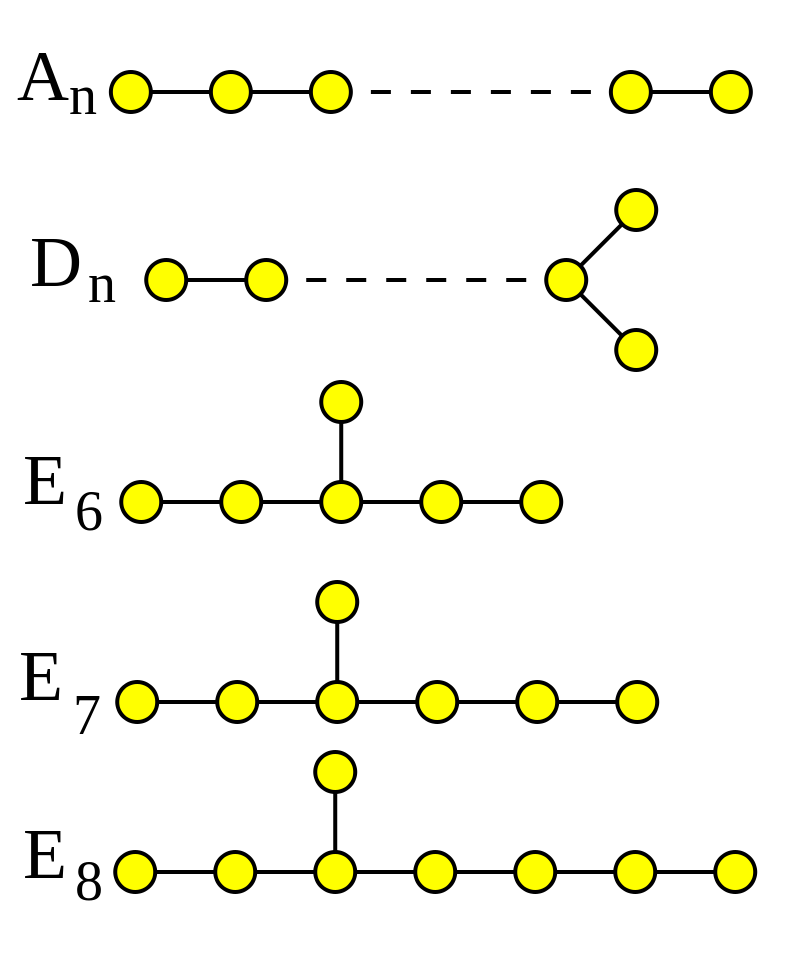
\includegraphics[scale=0.3]{images/simply_laced}
		\caption{Simply-laced Dynkin diagrams.}
	\end{center}
\end{figure}

\subsection{Examples of resolutions}
\begin{example}[ ]\label{}\text{}
Consider $x^4+y^4=z^2$.\footnote{Fermat showed that this equation has no integer solutions, demonstrating Fermat's last theorem for $n=4$.} Differentiating, one gets $4x^3=0$, $4y^3=0$, and $2z=0$. Therefore, the only singularity here is at $(0,0,0)$. Let us blow up the point $(0,0,0)$. Hence, we work in $\mathbf{A}^3\times \mathbf{P}^2$, introducing new coordinates $(X:Y:Z)$ in $\mathbf{P}^2$. We assert $xY=Xy$, $xZ=Xz$, and $yZ=Yz$. Cover $\mathbf{P}^2$ by three copies of $\mathbf{A}^2$ corresponding to $Z=1$, $Y=1$, and $X=1$. For the first case, one gets 
\begin{align*}
	z^2X^4+z^2Y^4=1.
\end{align*}
This is nonsingular. For the second case, one gets
\begin{align*}
	y^2X^4+y^2=Z^2.
\end{align*}
This has singularities whenever $y=Z=0$. A similar thing happens with $X=1$. (What's happening is that there is a projective line of singular points.)

\begin{remark}
	A singularity's ``complexity'' has more to do with its codimension than its dimension.
\end{remark}

Let us blow up $y^2X^4+y^2=Z^2$ along $y=Z=0$. Introduce coordinates $(s:t)$ where $sZ=ty$. With $s=1$, one gets 
\begin{align*}
	X^4 + 1=t^2,
\end{align*}
which is nonsingular. One also gets a nonsingular variety with $t=1$.
\end{example}


\begin{example}[Blowing up can make the singularity worse]\label{}\text{}
Consider $x^2-yz=0$. Instead of blowing up at the conical singularity $(0,0,0)$, blow up along $y=z=0$. Introduce coordinates $(Y:Z)$ of $\mathbf{P}^1$ where $yZ=Yz$. Take $Y=1$. Then, one gets
\begin{align*}
	x^2-y^2Z=0,
\end{align*}
which is the more complicated \index{Whitney umbrella}Whitney umbrella.
\end{example}

\begin{example}[ ]\label{}\text{}
The ring $\mathbf{Z}\!\left[\sqrt{-3}\right]$ does not have unique factorization:
\begin{align*}
	2\cdot 2 = (1+\sqrt{-3} ) (1-\sqrt{-3} ).
\end{align*}
Even though it is the coordinate ring of a scheme, pretend that $\mathbf{Z}\!\left[\sqrt{-3}\right]$ is the coordinate ring of a variety. This ring has a maximal ideal $(2,\sqrt{-3}-1 )$. If one, somehow, thinks of maximal ideals as points, one wants to show that the variety has a singular point at that maximal ideal. Let us look at the local ring $R=\Z_{(2)} \!\!\left[ \sqrt{-3}  \right] $ whose maximal ideal is $\mathfrak{m}=(2,\sqrt{-3}-1 )$. One sees that \begin{align*}
	R/\mathfrak{m} = \mathbf{F}_{2}.
\end{align*}
Further, $R/\mathfrak{m}^2$ has order $8$, so $\mathfrak{m}/\mathfrak{m}^2$ is a $2$-dimensional vector space over $R/\mathfrak{m}$. (Recall that $\mathfrak{m}/\mathfrak{m}^2$ is the \index{Zariski cotangent space}Zariski cotangent space at $\mathfrak{m}$.) The \index{Krull dimension}Krull dimension of $R$ is $1$ since the only prime ideals of $R$ are $(0)$ and its maximal ideals. One notices that this is smaller than the dimension of the cotangent space at $\mathfrak{m}$, so $\mathfrak{m}$ corresponds to a ``singular point.''

\begin{remark}
	The existence of a singular point is somehow related to unique factorization failing. However, there are some rings of algebraic integers with no singular points in which unique factorization fails. 
\end{remark}

Now, we will resolve this singularity. One can blow up, but we won't do that. To resolve a singularity in number theory, one might take the \defn{normalization}\index{normalization} (i.e. \defn{integral closure}\index{integral closure}) of the ring. The integral closure of $\Z\!\left[ \sqrt{-3}  \right] $ is
\begin{align*}
	\Z \!\left[ \frac{1+\sqrt{-3} }{2} \right] = \Z[\omega] .
\end{align*}
Since $\omega^2+\omega+1=0$, $\omega$ is an algebraic integer in the field of fractions of $\Z\!\left[ \sqrt{-3}  \right] $. This integral closure has unique factorization, and its points are nonsingular.
\end{example}

\begin{example}[Application of resolutions]\label{}\text{}
Recall that
\begin{align*}
	\Gamma(s) :=  \int_{0}^{\infty} e^{-t}t^{s-1}  \, dt
\end{align*}
	converges for $\Re (s)>0$ and can be extended to a meromorphic function of $s$ by integrating by parts. Suppose that $f(x_1,\hdots,x_n)$ is a polynomial and $\varphi(x_1,\hdots, x_n)$ is a smooth function with compact support. Then
	\begin{align*}
		\int_{0}^{\infty} \left\lvert f(x_1,\hdots, x_n) \right\rvert ^s\varphi(x_1,\hdots,x_n)  \, dx_1\cdots dx_n 
	\end{align*}
	will be a holomorphic function of $s$ for $s$ large enough. Can one continue this to all $s$? This is more or less the situation of $\Gamma$.\footnote{Let's ignore that $e^{-t}$ does not have compact support.} The problems here occur at the roots of $f$, which correspond to hypersurfaces with singularities.
	
	Atiyah suggested to use Hironaka's theorem to resolve the singularities of $\{f=0\}$. What one ends up with isn't really nonsingular, since blowing up introduces exceptional curves. These exceptional curves don't really matter, though, since they cross transversally. That is, when one blows up, one gets singularities $x_1\cdots x_k=0$ (one gets hyperplanes intersecting orthogonal to each other). Therefore, we reduce to 
	\begin{align*}
		\int_{}^{}  \left\lvert x_1\cdots x_n \right\rvert^s\varphi(x_1,\hdots,x_n)   \, dx_1\cdots dx_n =0.
	\end{align*}
	This splits into integrals of the form
	\begin{align*}
		\int\left\lvert x_1 \right\rvert ^sf(x_1)\, dx_1=0,
	\end{align*}
	which one can do with integration by parts, just as one does with $\Gamma$. Hence, one can continue integrals of the form above. Bernstein came up with a much more simpler way of showing this using Bernstein (or Bernstein--Sato) polynomials.
\end{example}

\subsection{Completions}
The completion of $R=k[x]$ is the formal power series ring $k[\![x]\!]$. \iffalse How does one get this, though? Take the ideal $I=(x)$. Then
\begin{align*}
	R/I&= k;\\
	R/I^2 &= \{a_0+a_1x:a_0,a_1\in k\};\\
	R/I^3 &= \{a_0+a_1x+a_2x^2:a_0,a_1,a_2\in k\};
\end{align*}
etc. An element One has a sequence
\[
\begin{tikzcd}
	\cdots \ar[r] &R/I^4\ar[r] &R/I^3\ar[r]&R/I^2 \ar[r] &R/I\\
		      &&\widehat{R}\ar[lu]\ar[u]\ar[ru]
\end{tikzcd}
\]
\fi Let's see how one gets this.

Consider the ideal $I=(x)$. Notice that there is a natural surjective map $\varphi_n :R/I^{n+1} \longrightarrow R/I^{n}$. One says that the sequence
\[
\begin{tikzcd}
	\cdots\ar[r] &R/I^{n+1}\ar[r,"\varphi_n"]&R/I^n \ar[r] &\cdots\ar[r] &R/I^2 \ar[r,"\varphi_1"] &R/I 
\end{tikzcd}
\]
forms a \defn{projective system}\index{projective system} indexed by the natural numbers.
The completion of $R$ at $I$ is the \defn{projective limit}\index{projective limit} or \defn{inverse limit}\index{inverse limit} of the system $(R/I^n, \varphi_n)$; that is, an element of the completion
\begin{align*}
	\widehat{R}_I = \widehat{R} := \varprojlim (R/I^n, \varphi_n)
\end{align*}
is a sequence $z=(\hdots, z_n,\hdots,z_1)$ with $z_n\in R/I^n$ and $\varphi_n (z_n)=z_{n-1}$ if $n\ge 2$. This naturally extends to all rings $R$ and their ideals.

\begin{example}[ ]\label{}\text{}
Let $p$ be a prime number. Take $R=\mathbf{Z}$ and $\mathfrak{p}=(p)$. Then the completion $\widehat{R}_\mathfrak{p} = \mathbf{Z}_p$ is the $p$-adic integers.
\end{example}

In algebraic geometry, one likes to consider the completion of a local ring $R$ at its maximal ideal $\mathfrak{m}$.

The natural map $R\longrightarrow \widehat{R}$ is injective if $R$ is Noetherian.

\begin{example}[The natural map does not need to be injective]\label{}\text{}
\begin{enumerate}
	\item Let $R$ be all smooth functions on $\mathbf{R}$.\footnote{Note that $R$ isn't local.} Let $I=(x)$ be functions vanishing at $0$. Then the completion $\widehat{R}_I$ is given by power series. However, the natural map is not injective: Consider
		\begin{align*}
			f(x):=
			 \begin{cases}
				 e^{-1/x^2}&x\ne 0\\
				 0&x=0,
			\end{cases}
		\end{align*}
		which is in the kernel of the natural map.
	\item Let $R = k [\![x,x^{1/2},x^{1/4},\hdots]\!]$. Let $I=(x,x^{1/2}, x^{1/4},\hdots)$. (Note that $I=I^2$.) Then $\widehat{R}_I = k$.
\end{enumerate}
\end{example}

An application of completions of rings is \defn{Hensel's lemma}\index{Hensel's lemma}. There are many different ``Hensel's lemmas'' that depend on the context, but here's the main idea: Solutions in $R/\mathfrak{m}$ can be lifted to solutions in $\widehat{R}$ under some conditions.

\begin{example}[Factorizing polynomials]\label{}\text{}
Suppose $f(z)\equiv g_0(z) h_0(z)\pmod{\mathfrak{m}}$ where $g_0,h_0\in k[z]$ and $f\in R[z]$. Then this lifts to a factorization $f(z)=g (z)h (z)$ in $R[z]$ if $g_0$ and $h_0$ are coprime in $k[z]$.
\end{example}

\begin{esquisse}
	Suppose $f\equiv gh\pmod{\mathfrak{m}^n}$. Try to find elements $a,b\in \mathfrak{m}^{n+1}/\mathfrak{m}^{n+2}$ such that $f\equiv (g+a) (h+b)\pmod { \mathfrak{m}^{n+1}}$. One needs to solve an equation $g_0b+h_0a = *$, which one can solve if $g_0$ and $h_0$ are coprime. (This is related to the fact that two coprime polynomials over a field generate the unit ideal.)
\end{esquisse}

\begin{example}[ ]\label{}\text{}
Consider the curve $y^2 = x^3+x^2$. Looking closely at its singularity, one wants to say that the curve is a union of lines that intersect there. However, one struggles to see this looking at the local ring. If the local ring allowed for this, then it would have zero divisors, and it doesn't. The local ring isn't ``aware'' that the curve seems to split into two components near the origin. However, the completion is. 

Let $R$ be the local ring at $(0,0)$. Let $\widehat{R} = k [\![x,y]\!]/(y^2-x^3-x^2)$. Notice that $y^2-x^3-x^2\equiv (y-x) (y+x)\pmod {I^3}$. One lifts this to a product of power series $(y-x+\cdots) (y+x+\cdots)$. This corresponds to the components.
\end{example}

\begin{remark}
	One says that the varieties $y^2=x^3+x^2$ and $y^2=x^2$ are \defn{analytically isomorphic}\index{analytic isomorphism}; that is, the completions of their local rings are isomorphic.
\end{remark}

\begin{remark}
	The completion $\widehat{R}$ has zero divisors though $R$ does not. There are examples of reduced rings whose completions are not reduced.
\end{remark}

\begin{remark}
	There is a variation on completion called \defn{Henselization}\index{Henselization} that is better behaved.
\end{remark}

One has the following maps:
\[
\begin{tikzcd}
	R\ar[r]&\widehat{R}\ar[r] &\cdots\ar[r] & R/\mathfrak{m}^2 \ar[r]& R/\mathfrak{m} = k.
\end{tikzcd}
\]
One can think of successive maps looking at a point in a finer neighbourhood.


\subsection{Resultants}
This section will concern elimination theory. Andr\'e Weil's \underline{Foundations of Algebraic Geometry} has an infamous footnote:
\begin{center}
	\small The device that follows, which, it may be hoped, finally eliminates from algebraic geometry the last traces of elimination-theory, is borrowed from C. Chevalley's Princeton lectures.
\end{center}
This is quite funny next to the following line from a poem by Shreeram Abhyankar:
\begin{center}
	\small Eliminate the eliminators of elimination theory!
\end{center}

		Suppose you have two polynomials, say $x^3y^4 - 7x^2-xy^8$ and $3x^2y^5+4y^2+x^4y^7$. Now, suppose you want to eliminate $y$. The variable $x$ should satisfy a polynomial of degree $9\cdot 11$. Here's the general problem: Suppose
		\begin{align*}
			f(x)&=a_mx^m+\cdots +  a_1x+a_0;\\
			g(x)&=b_nx^n+\cdots +  b_1x+b_0.
		\end{align*}
What is the condition for $f$ and $g$ to have a common root? Temporarily suppose that $a_m\ne 0$ and $b_n\ne 0$. Then the condition is $f(x)p (x)=g (x)q (x)$ where $\deg p<n$ and $\deg q<m$. If $f$ and $g$ have a common root $\alpha$, one has
\begin{align*}
	p(x)&= \frac{g(x)}{x-\alpha};\\
	q(x)&= \frac{f(x)}{x-\alpha}.
\end{align*}
The equation $f(x)p (x)=g (x)q (x)$ gives homogeneous linear equations. The condition for homogeneous equations having a nontrivial solution is that some determinant vanishes. What we want is the determinant of this matrix:
\begin{align*}
	\mat{a_m & \cdots & a_0 && &&\\ & a_m & \cdots & a_0& &&\\ &&&\ddots&&&\\&&&a_m & \cdots & a_0\\&&&&a_m & \cdots & a_0\\b_n & \cdots & b_0 && &&\\ & b_n & \cdots & b_0& &&\\ &&&\ddots&&&\\&&&b_n & \cdots & b_0\\&&&&b_n & \cdots & b_0 }.
\end{align*}
This $ (m+n)\times  (m+n)$ matrix is called the \defn{Sylvester matrix}\index{Sylvester matrix} and its determinant is called the \defn{resultant}\index{resultant}\footnote{The prefix ``ant'' indicates that the resultant is some invariant and that Sylvester probably named it.} of $f$ and $g$.

\begin{remark}\label{ifffffffffff}
	One can think of the case where the leading coefficient of a polynomial $f$ is $0$ as $f$ having a root at infinity: One expects
	\begin{align*}
		f(x) = a_mx^m+\cdots+a_1x+a_0
	\end{align*}
	to have $m$ roots, but it doesn't if $a_m=0$. One makes up for this by saying that $f$ has a root at infinity. One way to think about this is looking at the homogeneous polynomial
	\begin{align*}
		a_mx^my^0 + a_{m-1}x^{m-1}y^1+\cdots +a_1x^1y^{m-1} +a_0x^0y^m
	\end{align*}
	and considering a root to be a point $(x:y)\in  \mathbf{P}^1 = k\cup \{\infty\}$. The resultant is $0$ if and only if the homogenized polynomials have a common root in $\mathbf{P}^1$.
\end{remark}

\begin{example}[ ]\label{}\text{}
The polynomial $f(x)=ax^2+bx+c$ has a double root if it and its derivative have a root in common (this is true for all polynomials). Let $g(x)=2ax+b$ be the derivative of $f$. One sees that the resultant of $f$ and $g$ is
\begin{align*}
	\det\mat{a&b&c\\2a&b&0\\0&2a&b} = a(b^2-4ac).
\end{align*}
The factor $(b^2-4ac)$ is the well-known quadratic discriminant, and the factor $a$ corresponds to the case when the leading coefficient is $0$, as discussed in \cref{ifffffffffff}.  
\end{example}

\begin{example}[ ]\label{}\text{}
Let us see when $f(x)=x^3+bx+c$. Write $g (x)= 3x^2 + b$ for the derivative of $f$. Then the resultant of $f$ and $g$ is
\begin{align*}
	\det\mat{1&0&b&c&0\\0&1&0&b&c\\3&0&b&0&0\\0&3&0&b&0\\0&0&3&0&b}&= 4b^3+27c^2.
\end{align*}
Notice that the definition of the resultant allows for sign inaccuracy; indeed, the discriminant of a cubic is $-(4b^3+27c^2)$.
\end{example}

\subsection{Proper maps}
Suppose $f$ and $g$ are homogeneous polynomials in $z_1$ and $z_2$ with coefficients in $k[y_1,\hdots, y_\ell]$. One might think of $f$ and $g$ as hypersurfaces $H_f$ and $H_g$ in $\mathbf{A}^\ell\times \mathbf{P}^1$. Consider the projection $\mathbf{A}^\ell\times \mathbf{P}^1\longrightarrow \mathbf{A}^\ell$. The condition that the resultants of $f$ and $g$ vanish (that is, the condition that $f$ and $g$ have a common root in $\mathbf{P}^1$) is that a point is in the image of $H_f\cap H_g\longrightarrow \mathbf{A}^\ell$. The image comprises the roots of the resultant (a polynomial in $k[y_1,\hdots,y_\ell]$). This is closed.

\begin{remark}
	It is a common mistake to think that the image of a closed set under a projection is closed.
\end{remark}

\begin{example}[ ]\label{}\text{}
The projection $\mathbf{A}^1\times \mathbf{A}^1 \longrightarrow \mathbf{A}^1$ is not closed: Consider $\{xy=1\}\longmapsto \mathbf{A}^1-\{0\}$.
\end{example}

\begin{exercise}\label{}\text{}
Show that the image of a polynomial under $\mathbf{R}^n\longrightarrow \mathbf{R}$ does not need to be closed.
\end{exercise}

We have seen that $\mathbf{P}^n(\mathbf{R})$ and $\mathbf{P}^n(\mathbf{C})$ are compact in the usual topology. Projective space over a field is compact in the Zariski topology, but even affine space over a field is compact in this setting.

\begin{problem}
	What is the correct analogue of compactness?
\end{problem}

First, let us digress. A map of topological spaces $X\longrightarrow Y$ is \defn{proper}\index{proper map} if it is continuous and universally closed. (Recall that a map is \defn{universally proper}\index{universally proper morphism} if $X\times W\longrightarrow Y\times W$ is closed for all $W$.) Notice that this is equivalent to saying that $X\longrightarrow Y$ is continuous and closed and has compact fibres.

Maps of Hausdorff spaces are proper if and only if they are continuous and the preimage of a compact set is compact.

A map of varieties $X\longrightarrow Y$ is called \defn{proper}\index{proper map} if it is universally closed for the Zariski topology on the product $X\times Y$. 

Now, we have somewhat of an analogue: Saying that a map from $X$ to a point is proper is like saying that $X$ is compact. We would like to show that, if $X$ is a projective variety, then maps from $X$ to a point is proper. One can reduce this to showing that $\mathbf{P}^n\times \mathbf{A}^m\longrightarrow \mathbf{A}^m$ is closed.

First, let us show that $\mathbf{P}^1\times \mathbf{A}^m\longrightarrow \mathbf{A}^m$. Suppose that $S$ is closed in $\mathbf{P}^1\times \mathbf{A}^m$. Then $S$ is given by the roots of polynomials $f_1,\hdots, f_\ell$ in $x,y, z_1,\hdots,z_m$. Consider 
\begin{align*}
	&s_1f_1+s_2f_2+\cdots+s_\ell f_\ell;\\
	&t_1f_1+t_2f_2+\cdots+t_\ell f_\ell.
\end{align*}
These are homogeneous polynomials in $x$ and $y$ with coefficients that are polynomials in $s_1,\hdots,s_\ell,t_1,\hdots, t_\ell,z_1,\hdots, z_m$. The projection of $S$ to $\mathbf{A}^m$ is given by the points where these polynomials have a common root---given by roots of all of the coefficients of all of the monomials in $s_1,\hdots,s_\ell,t_1,\hdots, t_\ell$ of the resultant. One can show that this implies that a map from $\mathbf{P}^1$ to a point is proper.

Showing that maps from $\mathbf{P}^n$ to a point are proper would be straightforward if $\mathbf{P}^n$ was a product of $\mathbf{P}^1$s: One knows that maps from $\mathbf{P}^{n-1}\times \mathbf{P}^1$ to a point are proper, since
\begin{align*}
	\mathbf{P}^{n-1} \times \mathbf{P}^1\times X\longrightarrow X
\end{align*}
is closed. (This follows from $\mathbf{P}^{n-1}\times X\longrightarrow X$ being closed.) 

Even though $\mathbf{P}^n\ne \mathbf{P}^{n-1}\times \mathbf{P}^1$, one can still use this. The blow up of $\mathbf{P}^n$ at a point is a nontrivial $\mathbf{P}^1$-bundle over $\mathbf{P}^{n-1}$.\footnote{That is, it looks like a product of $\mathbf{P}^1$ and something even if it doesn't globally. There might be some ``twisting'' going on.} Let us show that this is true, first.

The map $\mathbf{P}^{n}\longrightarrow \mathbf{P}^{n-1}$ isn't defined everywhere, but is still a sort of correspondence. Consider the ``graph'' $G\subseteq \mathbf{P}^n\times \mathbf{P}^{n-1}$ of this map.\footnote{Note that this map is not a function.} This is the set of pairs $((x_0:\cdots:x_n), (y_1:\cdots:y_n))$ such that $x_iy_j=x_jy_i$ for all $i$ and $j$. The map $G\longrightarrow \mathbf{P}^n$ is an isomorphism except that it maps $\mathbf{P}^{n-1}$ to $(1:0:\cdots:0)$. This means that $G$ is the blowup of $\mathbf{P}^n$ at this point. Further, $G\longrightarrow \mathbf{P}^{n-1}$ is locally a map from a product of $\mathbf{P}^1$ and an affine set to the same affine set. Thus, $G\longrightarrow \mathbf{P}^{n-1}$ is proper.

One gets the diagram
\[
\begin{tikzcd}[column sep = 8 em, row sep = 5 em]
	G \ar[r, "\textrm{surjective}" \iffalse twoheadrightarrow\fi] \ar[d,swap,"\textrm{proper}"] \ar[dr, "\textrm{proper}"] & \mathbf{P}^n\ar[d]\\
	\mathbf{P}^{n-1}\ar[r,"\textrm{proper }\\ \textrm{by induction}", swap] &\textrm{point,}
\end{tikzcd}
\]
whence it follows that the rightmost arrow is proper.

\begin{remark}
	This illustrates the technique of using blow up to turn a rational map into a regular map.
\end{remark}

\begin{remark}
	For $n=2$, the set $G$ is called a \defn{ruled surface}\index{ruled surface} over $\mathbf{P}^1$; that is, it is a surface $G$ where the fibres of $G\longrightarrow \mathbf{P}^1$ are copies of $\mathbf{P}^1$. The set $\mathbf{P}^1\times \mathbf{P}^1$ is also a ruled surface over $\mathbf{P}^1$.\footnote{Ruled surfaces over $\mathbf{P}^1$ are \index{Hirzebruch surface}Hirzebruch surfaces.}
\end{remark}

\subsection{Survey of curves}
Algebraic curves over $\mathbf{C}$ are birational to nonsingular projective curves. These are more or less the same as compact Riemann surfaces. They also correspond to finitely-generated fields over $\mathbf{C}$ of transcendence degree $1$.\footnote{One goes from a nonsingular projective curve to a field by taking rational functions. See p. 39 of Hartshorne's \underline{Algebraic Geometry} for the other direction.} Of course, there is a correspondence between compact Riemann surfaces and function fields of dimension $1$.

The principal invariant of curves is the \defn{genus}\index{genus}. One talks about the genus for compact Riemann surfaces since one already has the notion of genus for orientable topological surfaces. For every genus, one has a \defn{moduli space}\index{moduli space} whose points are the isomorphism classes of curves of that genus.

The only curve\footnote{That is, nonsingular projective curve.} of genus $0$ is $\mathbf{P}^1$, so the moduli space of curves of genus $0$ has one point.

Genus-$1$ curves are called \defn{elliptic curves}\index{elliptic curve}. If one looks at curves as compact Riemann surfaces, any elliptic curve can be written as $\mathbf{C}/\Lambda$ where $\Lambda$ is a lattice. The Weierstrass $\wp$ function, which satisfies
\begin{align*}
	(\wp') ^2 = 4\wp^3 -g_2\wp-g_3,
\end{align*}
maps $\mathbf{C}/\Lambda$ to the algebraic curve $y^2=4x^3-g_2x-g_3$. There is a two-to-one map from this curve to the plane that ramifies at four points: the three roots of the equation and a point at infinity.

Given three points $\lambda_1,\lambda_2,\lambda_3$ in the projective line, there is a linear fractional transformation 
\begin{align*}
	\tau\longmapsto \frac{a\tau+b}{c\tau+d}
\end{align*}
that takes $\lambda_1$ to $0$, $\lambda_2$ to $1$, and $\lambda_3$ to $\infty$. A fourth point $\lambda_4$ will be taken to some $\lambda$. Thus, any elliptic curve is defined by a number $\lambda$ and the equation $y^2=x(x-1) (x-\lambda)$. Different values of $\lambda$ can give the same algebraic curve: There is a group of order $6$ permuting $0$, $1$, and $\infty$ given by one of these transformations:
\begin{align*}
	\lambda&\longmapsto\lambda;\\
	\lambda&\longmapsto 1-\lambda;\\
	\lambda&\longmapsto\frac{1}{\lambda};\\
	\lambda&\longmapsto \frac{1}{1-\lambda};\\
	\lambda&\longmapsto \frac{\lambda}{\lambda-1};\\
	\lambda&\longmapsto 1-\frac{1}{\lambda}.
\end{align*}
This group is isomorphic to $\Sg_3$. Hence, the moduli space of elliptic curves is given by the affine line parameterized by $\lambda$ modulo $\Sg_3$. An invariant under this action is the \index{$j$-invariant}$j$-invariant of the elliptic curve $y^2 = x(x-1) (x-\lambda)$:
\begin{align*}
	j(\lambda) := \frac{256(\lambda^2-\lambda+1)^3}{\lambda^2(\lambda-1)^2}.
\end{align*}

However, one can also write an elliptic curve as $\mathbf{C}/\Lambda=\mathbf{C}/\langle 1,\tau\rangle$. That is, given $\tau$, one should have a $j$-invariant. If $q=e^{2\pi i\tau}$, one has
\begin{align*}
	j(\tau) := q ^{-1} + 744 + 196884q + \cdots.
\end{align*}

Elliptic curves are isomorphic if and only if they have the same $j$-invariant, so one might say that the moduli space of elliptic curves is, more or less, the affine line. However, this moduli space isn't a variety at all; it is an \defn{algebraic stack}\index{algebraic stack}. Describing moduli spaces of things that have automorphisms is kind of difficult.

Let us move on to genus-$2$ curves. One considers the equation
\begin{align*}
	y^2 = (x-a_1)(x-a_2)(x-a_3)(x-a_4) (x-a_5) (x-a_6).
\end{align*}
One takes $6$ points in $\mathbf{C}$ and a curve that is ramified to order $2$ over these points. In general,
\begin{align*}
	y^2 = (x-a_1)\cdots (x-a_{2n})
\end{align*}
has Euler characteristic $\chi = 2+2n-4n +2 = 4-2n$, so its genus is $g=n-1$ (since $\chi = 2-2g$). Curves of the form above are called \defn{hyperelliptic curves}\index{hyperelliptic curve}. All genus-$2$ curves are hyperelliptic. Classifying genus-$2$ curves is equivalent to taking $6$ distinct points in $\mathbf{P}^1$ modulo the action of the group $\PSL_{2}(\mathbf{C})$ given by
\begin{align*}
	\tau \longmapsto \frac{a\tau+b}{c\tau+d}.
\end{align*}
This is, more or less, the same as classifying binary forms of degree $6$ modulo the action of $\SL_{2}(\mathbf{C})$. This comes down to the problem of classifying the invariance of binary quantics. One gets that this looks like $\mathbf{A}^3/(\mathbf{Z}/5\mathbf{Z})$ where $\mathbf{Z}/5\mathbf{Z}$ acts by
\begin{align*}
	(x,y,z) \longmapsto  (\zeta x,\zeta^2 y, \zeta^3 z)
\end{align*}
where $\zeta$ is a $5$th root of unity. The set of generators for the invariants of this action is $\{x^5,x^3y,xy^2,y^5,x^2z, xz^3, z^5, yz\}$. Hence, there is an explicit description of the moduli space genus-$2$ curves, though a messy one. 

We continue to consider curves of genus $3$. There are hyperelliptic genus-$3$ curves and degree-$4$ nonsingular curves in the plane. One can determine the genus of a nonsingular plane curve of degree $d$: One can think of a generic degree-$d$ plane curve as a $d$-fold cover of the line and, generally, it will have $d(d-1)$ $2$-fold branch points and only $2$-fold branch points. Therefore, its Euler characteristic is $\chi = 2d -  d(d-1)$, so its genus is $(d-1) (d-2)/2$. Hence, the genus of nonsingular plane curve must be a triangular number.

There is a $6$-dimensional family of degree-$4$ nonsingular plane curves. The hyperelliptic curves form a family of dimension $5$.
\begin{figure}
        \begin{center}
                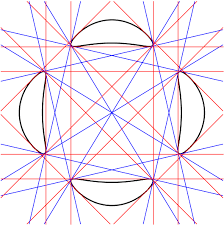
\includegraphics{images/trott_curve.png}
                \caption{The Trott curve and its $28$ bitangents.}
        \end{center}
\end{figure}
\begin{example}[Trott curve]\label{}\text{}
The \defn{Trott curve}\index{Trott curve} is given by
\begin{align*}
	12^2(x^4+y^4) - 15^2 (x^2+y^2) + 350 x^2y^2+81=0.
\end{align*}
This is a simple example of a nonsingular genus-$3$ curve with $28$ bitangents.
\end{example}

Curves of genus $4$ are intersections of a cubic and quadric in $\mathbf{P}^3$. Curves of genus $5$ are intersections of three quadrics in $\mathbf{P}^4$.

\subsection{Hurwitz curves}
Hurwitz curves are the most symmetric curves of a given genus $g$. The group of automorphisms for the cases $g=0$ and $g=1$ are infinite. Thus, we would like to consider the automorphism group $G$ of curves of genus $g>1$. Hurwitz proved that
\begin{align*}
	\# G \le 84(g-1)
\end{align*}
in characteristic $0$. 
\begin{esquisse}
	Consider the orbifold Euler characteristic. Recall that the Euler characteristic is $\chi =n_2-n_1+n_0$ where $n_i$ is the number of cells of dimension $i$ (in a suitable cellular decomposition). The Euler characteristic of a compact orientable surface is $\chi = 2-2g$. An \defn{orbifold}\index{orbifold} is the quotient of a surface by a finite group.\footnote{That is, it is for our purposes.} If one has a point fixed by a subgroup $H$, then the quotient of this point by $H$ might be thought of as $1/\# H$ of a point. \iffalse Consider the unit disk. Take the automorphism of order $2$ that corresponds to a rotation by $\pi$. If\fi One can check that, if $S$ is a surface and $G$ is a finite group,
	\begin{align*}
		\chi(S/G) =  \frac{\chi(S)}{\# G}.
	\end{align*}
One can consider $S/G$ a surface, provided the action of $G$ is ``nice'' enough. That is, $S/G$ has a topological Euler characteristic and an orbifold Euler characteristic. Suppose that $S/G$ is a surface $T$ with conical singular points of orders $p_1,p_2,\hdots, p_m$. The orbifold Euler characteristic is the topological Euler characteristic minus $\sum_{i}^{}  (1-1/p_i)$.\footnote{What is happening here is that each conical singularity contributes $1$ to the topological Euler characteristic and $1/p_i$ to the orbifold one.} We want to show that the maximal value of the orbifold Euler characteristic is $-1/42$.

First, note that the topological Euler characteristic is $2-2h$ where $h$ is genus of the topological surface. One sees that $h=0$, since the orbifold Euler characteristic must be negative.\footnote{Recall that $g>1$.} Suppose that there are at most $2$ conical points $p_1$ and $p_2$. Then, again, the orbifold Euler characteristic will be positive. Suppose there are at least $4$ conical points. Then the orbifold Euler characteristic will be at most $-1/6$ (since $0$ is not possible), which is less than $-1/42$. Therefore, we look at the case where there are $3$ conical points $p_1$, $p_2$, and $p_3$. 

Suppose that there are no conical points of order $2$. If each point has an order of $3$, then the orbifold Euler characteristic is $0$. If two points are of order $3$ and one is of order $4$, then it is $-1/12< -1/42$. Thus, there is at least $1$ point of order $2$. One also sees that there cannot be more than $2$ points of order $2$, since that makes the orbifold Euler characteristic positive. That is, there is $1$ point of order $2$.

Suppose $p_2,p_3\ge 4$. If one has equality, then the orbifold Euler characteristic is $0$. If $p_2=4$ and $p_3=5$, then the orbifold Euler characteristic is $-1/20<-1/42$. Thus, one can assume that $p_1=2$, $p_2=3$, and $p_3\ge 3$. The possibilities for $p_3$ give
\begin{align*}
	\frac{1}{6},\ \frac{1}{12},\ \frac{1}{30},\ 0, \ -\frac{1}{42},\  -\frac{1}{24},\ \hdots
\end{align*}
for the orbifold Euler characteristic.

Therefore, if $\chi<0$, then $\chi\le -1/42$. Further, if $\chi \ne -1/42$, then $\chi \le -1/24$. Hence, if the orbifold Euler characteristic is negative (that is, if $g>1$), then 
\begin{align*}
	\frac{2-2g}{\# G}\le -\frac{1}{42}.
\end{align*}
This implies
\begin{align*}
	\# G\le 84(g-1).
\end{align*}
\end{esquisse}
In particular, $G$ is generated by $\alpha$, $\beta$, and $\gamma$ where $\alpha^2=1$, $\beta^3=1$, $\gamma^7=1$, and $\alpha\beta\gamma=1$. A finite group $G$ generated by $3$ elements with these properties is called a \defn{Hurwitz group}\index{Hurwitz group}.

 \begin{definition}[ ]\label{}\text{}
A \defn{Hurwitz curve}\index{Hurwitz curve} is a genus-$g$ curve with $84(g-1)$ automorphisms.
\end{definition}

\subsection{Examples of Hurwitz curves}
One gets interesting information about genus $0$ or $1$ from the arguments of the previous section. If the genus is $g=0$, then the orbifold Euler characteristic is positive. The smallest orbifold Euler characteristic one gets is 
\begin{align*}
	2-\frac{1}{2}-\frac{2}{3}-\frac{4}{5}= \frac{1}{30} = \frac{2}{\# G}.
\end{align*}
This implies that there is a group of automorphisms of order $60$ that acts on $\mathbf{P}^1$. 

If $g=1$, then $\chi=0$. One can get this if there are no conical singularities, $4$ conical singularities of order $2$, $3$ conical singularities of order $3$, $1$ conical singularity of order $2$ and $2$ of order $4$, or $3$ conical singularities where the orders are $2$, $3$, and $6$.\footnote{These possibilities correspond to finite cyclic groups of orders $1$, $2$, $3$, $4$, and $6$ acting on an elliptic curve.} 

		Let us try to find the ``most symmetric'' curve of genus $g=2$. First, note that there isn't a genus-$2$ curve whose automorphism group has order $84$: Suppose that the automorphism group $G$ has order $84$. By the Sylow theorems, $G$ has a normal subgroup of order $7$. The group $G$ modulo this group of order $7$ is of order $12$ and has a normal subgroup of order $3$ or $4$. If it is of order $4$, then every element of order $2$ or $7$ is in the normal subgroup of order $28$, which has no elements of order $3$. Recall that any Hurwitz group has generators such that $\alpha^2 = \beta^3 = \gamma^7 = \alpha\beta\gamma = 1$. Therefore, one does not have a normal subgroup of order $4$. The order-$3$ normal subgroup case is similar: Every element of order $3$ or $7$ is contained in the normal subgroup of order $21$. Therefore, there is no Hurwitz group of order $84$.

		We also saw that if $\# G\ne 84(g-1)$, then $\# G \le 48(g-1)$. One sees that there is a curve whose automorphism group has order $48(g-1)=48$: Consider the double branched cover of $\mathbf{P}^1$ branched over $0$, $\infty$, $1$, $-1$, $i$, and $-i$.\footnote{One might think of these points as the vertices of an octahedron.} The subgroup of $\PSL_2(\mathbf{C})$ fixing these points is generated by
		\begin{align*}
			z&\longmapsto iz;\\
			z&\longmapsto \frac{z+1}{1-z}.
		\end{align*}
		Indeed, these generate a group of order $24$. The group of automorphisms is a central extension of this group in which the two branches are exchanged. This gives a group of order $48$ that acts on this hyperelliptic curve.

		There is a genus-$3$ Hurwitz curve that is given by the \defn{Klein quartic}\index{Klein quartic}:
		\begin{align*}
			x^3y + y^3z + z^3x=0.
		\end{align*}
		Indeed, this is nonsingular, and it is the only genus-$3$ curve whose automorphism group has order $84(g-1)=168$ up to isomorphism. Further, this automorphism group is the simple group $\PSL_{2}(\mathbf{F}_{7})$.\footnote{This is the smallest simple group after $\Ag_5$.} There is a manifest order-$3$ automorphism: $x\longmapsto y\longmapsto z\longmapsto x$. One also has order-$7$ automorphisms given by
		\begin{align*}
			x&\longmapsto \zeta^4x;\\
			y&\longmapsto \zeta^2y;\\
			z&\longmapsto \zeta z;
		\end{align*}
		where $\zeta$ is a $7$th root of unity. Determining the remaining automorphisms is quite difficult and, hence, omitted.

\begin{remark}
	In characteristic $p\ne 0$, the Euler characteristic behaves much differently than it does in characteristic $0$.\footnote{One defines the Euler characteristic in characteristic $p$ using \'etale cohomology.} Hence, the Hurwitz bound does not hold: The double cover of the projective line $y^2=x^p-x$ branched at all points defined over $\F_p$ has genus $g = (p-1)/2$ but is acted on by the group $\SL_{2}(\Z/p\Z)$ of order $p^3-p$.
\end{remark}

\subsection{Resolution of curve singularities}
We have seen that function fields of transcendence degree $1$ sort of correspond to nonsingular projective curves.\footnote{Hartshorne constructs a curve directly from a function field.} 

If a function field has transcendence degree $1$, then it is of the form $k(x,y)$ where $x$ is transcendental over $k$ and $f(x,y)=0$ for some $f$, which gives a possibly singular projective curve. We shall demonstrate that one can resolve the singularities of $f(x,y)=0$ by repeated blow ups.\footnote{We assert $\chr k =0$, though the result holds in all characteristics.}

Assume that the singular point is $(0,0)\in  \mathbf{A}^2$. Consider the lowest-degree terms, say $a_ny^n + a_{n-1}xy^{n-1} + \cdots + a_1 x^{n-1}y + a_0 x^n$. The number $n$ is the \defn{multiplicity}\index{multiplicity of a singularity} of the singularity. The roots of this homogeneous polynomial given by the lowest-degree terms are in $\mathbf{P}^1$ and correspond to the ``directions'' of the singularity. Blowing up this point means separating these directions. Therefore, $1$ blow up reduces multiplicities unless all of the points are the same. In the latter case, this homogeneous polynomial is of the form $a_n(y+\alpha x)^n$.

Make the change of variables $y\longmapsto y-\alpha x$. Then, the degree-$n$ terms are given by only $y^n$.

\begin{example}[ ]\label{}\text{}
Let us blow up $y^2+x^9 + x^3y^5$ at $(0,0)$. This corresponds to either $x\longmapsto xy$, which does not produce any singularities, or $y\longmapsto xy$. In this case, one gets
\begin{align*}
	y^2 + x^7 + x^6y^5=0.
\end{align*}
One sees that, under this change of variables, monomials of the form $y^nx^\alpha$ are invariant (by $y^nx^\alpha\longmapsto y^nx^{\alpha+n}$ and dividing out by the common $x^n$). In general, one has $y^{n-\ell}x^\alpha \longmapsto y^{n-\ell}x^{\alpha-\ell}$. Hence, one can blow up until at least $1$ monomial has degree $n$. Then, one is in the previous case in which multiplicities can be reduced by blowing up.
\end{example}

However, one sees that the monomials of degree $n$ might be another $n$th power. Nevertheless, either the process terminates or the polynomial is transformed into a power series. In the latter case, the original polynomial is divisible by some $m$th power of a power series where $m\ge 2$.\footnote{An example of this is $f(x,y)= (y^2-y+x^2)^2$.} This is not possible, though, since the original polynomial $f(x,y)$ doesn't have repeated factors.\footnote{It is actually an irreducible curve.} Therefore, one has an algorithm for resolving singularities of an algebraic curve by blowing up.

\begin{remark}
	Subschemes can be defined by a polynomial with repeated factors; in this case, their singularities cannot be resolved by blowing up.
\end{remark}

\subsection{Newton's rotating ruler}
Consider a polynomial $f(x,y)\in  \mathbf{C}[x,y]$ that is not a polynomial in $x$. Newton proved that $y$ is a power series in $x^{1/N}$ for some $N$. These are called \defn{Puiseux series}\index{Puiseux series}.\footnote{Puiseux series can have negative exponents, too.}

\begin{example}[ ]\label{}\text{}
If $f(x,y) = y^2-x^2 -x^3$, then
\begin{align*}
	y &= x\sqrt{1+x}\\
	  &= x \left( 1 + \frac{1}{2}x^{1/2} + \cdots \right). 
\end{align*}
\end{example}

\begin{esquisse}
	Suppose that $f$ has a $y^n$ term but not $y^i$ for $i<n$. Draw a square lattice of monomials. Mark all monomials $x^iy^j$ that occur in $f$. Get a ruler.\footnote{This ruler will become Newton's rotating ruler.} Place it vertically on the left of the lattice. Rotate it counterclockwise about the $y^n$ point until it reaches the first marked point. Draw a line through these points. Rotate about this point. Repeat. This process will generate a \defn{Newton polygon}\index{Newton polygon}.

	One notices that the line that one draws might not pass through a point on each horizontal. Hence, one introduces extra points by $x\longmapsto x^{1/r}$ for a suitable $r$. Write the next monomial through which the line crosses $y^{n-1}x^m$. One can call the terms on the first line of the Newton polygon (which, now, passes through a point on each horizontal) the ``smallest-degree terms.'' Put $\deg y = m$ and $\deg x = 1$. The monomials on this line give a homogeneous polynomial in $y$ and $x^m$. Factorize this to $(y-\alpha x^m) (y-\beta x^m)\cdots$. Then, with $y\longmapsto y+\alpha x^m$, this polynomial becomes $y(y-\gamma x^m)\cdots$. Notice that there is no term in $x^{mn}$.

	Now, with $y\longmapsto x^my$, all of the terms are divisible by $x^{mn}$, so one divides out by $x^{mn}$. One sees that all of the points on that line are pushed all the way to the left. Now, if any of the coefficients are nonzero, then the exponent on $y$ is less than $n$; then, one repeats with this smaller exponent. This happens when the first root in the factorization has multiplicity less than $n$. Hence, one focuses on the case when the multiplicity of this root is $n$.\footnote{Typically, this occurs when $n=1$.}

	In this case, the coefficient on $y^n$ is $1$. Further, every other coefficient on the line is $0$. Then, Newton's ruler has not met a marked point, so it rotates on. Therefore, either $n$ is decreased or the ruler is rotated counterclockwise. This rotation process\footnote{The rotation process here corresponds to $y\longmapsto y + *x^m$.} either continues ad infinitum or the smallest power of $y$ is reduced. There are finitely many times that one can reduce the exponent on $y$, so the rotation process will continue forever.

	When it continues on and on, one sees that the following sequence of variable changes is happening:
	\begin{align*}
		y &\longmapsto y + *x;\\
		y &\longmapsto y + *x^2;\\
		y &\longmapsto y + *x^3;
	\end{align*}
	etc. That is, one has $y\longmapsto y + *x + *x^2 + *x^3 + \cdots$. Then, all monomials $y^ix^j$ for $i< n$ vanish. Now, the series is divisible by $y$, so the original $f(x,y)$ is divisible by $y$ minus some power series in $x^{1/r}$ for some $r$. Thus, $y$ is a power series in $x^{1/r}$ that satisfies $f(x,y)=0$.
\end{esquisse}

\begin{corollary}[ ]\label{}\text{}
The field of Puiseux series 
\begin{align*}
	K = \bigcup_{n>0} \mathbf{C} (\!(x^{1/n})\!)
\end{align*}
is algebraically closed.
\end{corollary}

If one has a polynomial in $y$ whose coefficients are Puiseux series in $x$, its roots are Puiseux series. That is, $K$ is algebraically closed.

The field $K$ is a \defn{quasifinite field}\index{quasifinite field}. That is, its absolute Galois group is $\widehat{\mathbf{Z}}$, which is the absolute Galois group of $\mathbf{F}_{p}$.

\subsection{Hilbert polynomials}
Suppose $M=\bigoplus_{n}M_n$ is a finitely-generated graded module over a graded ring $R = k[z_1,\hdots, z_m]/I$ where $\deg z_i = d_i >0$. If $R$ is the graded ring of some projective variety, the ``growth rate'' of the $M_n$s might give some information about the variety.

Consider
\begin{align*}
	f_M(z) :=  \sum_{n}^{} z^n\dim_k(M_n)
\end{align*}
where $\dim_k(M_n)$ is the dimension of $M_n$ as a $k$--vector space. First, notice that $f_M$ is a \index{rational function}rational function. Consider the exact sequence
\[
\begin{tikzcd}
	0\ar[r]&\ker z_m \ar[r] & M \ar[r,"\times z_m"]& M(d_m) \ar[r] & M(d_m)/z_m M \ar[r]& 0. 
\end{tikzcd}
\]
Note that $M(d_m)$ means $M$ with its grading shifted by $d_m$. Since this is an exact sequence of vector spaces, one gets a relation between the dimensions of these vector spaces. Furthermore, $\ker z_m$ and $M(d_m)/z_m M$ are $R/(z_m)$-modules. Also,
\begin{align*}
	f_{M(d_m)}(z) = z^{d_m} f_M(z).
\end{align*}
Thus, by induction, $(1-z^{-d_m})f_M$ is a rational function. Further, $f_M$ is a rational function with denominator dividing $(1-z^{d_1})\cdots(1-z^{d_m})$.

Let us focus on the case $d_i=1$ for all $i$. Then, the denominator is $(1-z)^m$, and the coefficients of $x_i$ for $i\ge 0$ in the expansion of $1/(1-z)^m$ are given by a polynomial in $i$. Therefore, $\dim_k (M_n)$ is a polynomial in $n$ for $n>0$ large. This is called the \defn{Hilbert polynomial}\index{Hilbert polynomial} of $M$. It describes how rapidly the graded pieces of $M$ grow in large degree.

Write $g(n) := \dim_k(M_n)$ for the Hilbert polynomial of $M$. Though its coefficients are not necessarily integers, the restriction
\begin{align*}
	g:\mathbf{Z}\longrightarrow \mathbf{Z}
\end{align*}
is well defined; that is, $g$ is integer-valued. Let us see what integer-valued polynomials look like. Clearly, $a_mz^m + \cdots + a_1z + a_0$ is an integer if $z$ is an integer and $a_i$ is an integer for all $i$. However, an integer-valued function does not need integral coefficients: Consider
\begin{align*}
	\frac{z(z-1)}{2}.
\end{align*}

Notice that the binomial coefficients
\begin{align*}
	1 &= \binom{z}{0};\\
	z &= \binom{z}{1};\\
	\frac{z(z-1)}{2} &= \binom{z}{2};\\
	\frac{z(z-1) (z-2)}{3!}&= \binom{z}{3};
\end{align*}
are integer-valued. We shall demonstrate that these span the integer-valued polynomials. Write 
\begin{align*}
	g_n(z) := \binom{z}{n}.
\end{align*}
Then
\begin{center}
	\begin{tabular}{cccccccc}
		$z$&0&1&2&3&4&5\\
    		\midrule
		 $g_0(z)$& $1$ &     &     &    \\
		 $g_1(z)$& $0$ & $1$ &     &    \\
		 $g_2(z)$& $0$ & $0$ & $1$ &    \\
		 $g_3(z)$& $0$ & $0$ & $0$ & $1$\\
		 $g_4(z)$& $0$ & $0$ & $0$ & $0$ & $1$\\
		 $g_5(z)$& $0$ & $0$ & $0$ & $0$ & $0$ & $1$
	\end{tabular}
\end{center}
Suppose $f(n)$ is a degree-$\ell$ integer-valued polynomial. Then, one can choose coefficients such that
\begin{align*}
	f(n) -  a_0g_0(n) -  a_1g_1(n) - \cdots - a_\ell g_\ell (n) =0
\end{align*}
for $n = 0,\hdots, \ell$. The above is a polynomial of degree $\ell$ that vanishes at $\ell + 1$ points, so it is $0$. Notice that the leading coefficient of $f$ is $a_\ell n^\ell / \ell!$ where $a_\ell$ is an integer.\footnote{This integer will give the degree of projective varieties.}

\begin{remark}
In the construction of the Hilbert polynomial, we used $\dim_k(M_n)$ because it was additive on short exact sequences. Any other measure of the ``size'' of $M_n$ that is additive on short exact sequences can give a variation on the Hilbert polynomial of $M$.	
\end{remark}

\subsection{The degree of a projective variety}
\index{degree of a projective variety}
Suppose that $V\subseteq \PP^n$ is a projective variety. If $V$ is a hypersurface, it is given by $f(x_0,\hdots,x_n)=0$ for a polynomial $f$. One defines
\begin{align*}
	\deg V := \deg f.
\end{align*}

\iffalse
Most of the time, if $V$ has codimension greater than $1$, then $\deg V$ is the number of intersection points of $V$ with a hyperplane section $H$ or the number of intersections of $V$ with a linear variety of codimension $\dim V$. However, one requires the hyperplane section or linear variety to be in ``general position,'' whatever that means.
\fi

One used to define $\deg V$ in terms of intersections with hyperplane sections or linear varieties, but these ``definitions'' had many caveats to them.

Suppose $V$ corresponds to an ideal $I$ of $k [x_0,\hdots, x_n]=R$ (that is, $V$ is the set of roots of $I$). Now, $R/I$ is a graded ring, so it has a Hilbert polynomial. The degree of this Hilbert polynomial is $\dim V$. This is closely related to the following theorem from commutative algebra.

\begin{theorem}[ ]\label{}\index{}\text{}
Let $R$ be a local ring with maximal ideal $\mathfrak{m}$. Then $\dim R$ is $1$ plus the degree of the Hilbert polynomial of $\mathfrak{m}^n / \mathfrak{m}^{n+1}$.
\end{theorem}

If $d:=\dim V$, the leading coefficient of the Hilbert polynomial is $\alpha z^d/d!$ where $\alpha\in \Z$. One defines
\begin{align*}
	\deg V := \alpha.
\end{align*}
Notice that $\alpha>0$ since the Hilbert polynomial takes on positive values for large inputs.

\begin{remark}
	The degree defined this way is a well-defined invariant of a projective variety together with its embedding in projective space.
\end{remark}

\begin{example}[ ]\label{}\text{}
Suppose $V=\mathbf{P}^n$. Hence, one considers the graded ring $k[x_0,\hdots,x_n]/(0)=k[x_0,\hdots,x_n]$. The Hilbert polynomial of this is
\begin{align*}
	\binom{n+z}{n} = \frac{z^n}{n!} + \cdots.
\end{align*}
(This counts the monomials of degree $z$.) One sees that $\dim V = n$ and $\deg V = 1$. 
\end{example}

\begin{example}[ ]\label{}\text{}
Consider a hypersurface of a degree-$d$ polynomial $f(x_0,\hdots, x_n)$. Now, one considers $k[x_0,\hdots, x_n]/(f)$. The Hilbert polynomial of this is
\begin{align*}
	\binom{n+z}{n} - \binom{n+z-d}{n}  = d \frac{z^{n-1}}{(n-1)!} + \cdots,
\end{align*}
so the dimension of the hypersurface is $n-1$ and the degree of the hypersurface is $d$.
\end{example}

\begin{example}[Twisted cubic]\label{}\text{}
\index{twisted cubic} Recall that the twisted cubic is given by
\begin{align*}
	wz &= xy;\\
	x^2 &= wy;\\
	y^2 &= xz.
\end{align*}
One can kill off $x^2$, $y^2$, and $xy$, so a basis for the relevant quotient ring is $\{w^iz^{z- i}, w^ixz^{z- i -1}, w^iyz^{z-i-1}\}$. There are $( z+ 1)+z +  z = 3z + 1$ of these, so the Hilbert polynomial is $3z+1$. Therefore, the twisted cubic has dimension $1$ and degree $3$.
\end{example}

\begin{remark}
	The twisted cubic is isomorphic to the projective line, which is of degree $1$. Thus, the degree depends on the embedding.
\end{remark}

The \defn{Euler polynomial}\index{Euler polynomial} of $V$, $\chi(V)$, is the constant term of the Hilbert polynomial. The Euler polynomial depends on only the abstract variety, not on the variety's embedding. It is the Euler characteristic of the sheaf of rings of $V$. People didn't use $\chi(V)$; they used the \defn{arithmetic genus}\index{arithmetic genus}:
\begin{align*}
	(-1)^{\dim V}  (\chi(V)-1).
\end{align*}
The Euler characteristic is ``better,'' though, since
\begin{align*}
	\chi(V\times W) = \chi (V)\chi (W).
\end{align*}

\begin{problem}
	Determine the arithmetic genus of a plane curve of degree $d$.
\end{problem}

The Hilbert polynomial of this plane curve is
\begin{align*}
	\binom{2+z}{2} - \binom{2+z-d}{2} = dz + 1 - \frac{(2-d) (1-d)}{2},
\end{align*}
so the arithmetic genus is $(2-d) (1-d)/2$.

Robin Hartshorne proved the following theorem.\footnote{``Connectedness of the Hilbert scheme,'' 1963.}

\begin{theorem}[Hartshorne]\label{}\index{}\text{}
Let $S$ be a Noetherian prescheme, let $n$ be an integer, and let $p(z)\in\Q [z]$ be a polynomial. If $S$ is connected, then the Hilbert scheme $\Hilb^p(\mathbf{P}^n_S/S)$ is connected.
\end{theorem}

This implies that the Hilbert polynomial is, essentially, the only continuous invariant of things in projective space.

\subsection{B\'ezout's theorem}
Here is B\'ezout's theorem in its simplest form.
\begin{theorem}[B\'ezout]\label{b_1}\index{B\'ezout's theorem}\text{}
Curves of degrees $m$ and $n$ intersect at $mn$ points.
\end{theorem}
However, this is wrong as stated. Two distinct parallel lines, for example, do not intersect. To patch this, one includes points at infinity (that is, one works in projective space). The curves $y=0$ and $y=x^2+1$ do not intersect over $\R$, but they do over $\C$. Thus, one needs to work over an algebraically closed field. Thirdly, the curves must not have components in common. Further, the curves $y=0$ and $y=x^2$ intersect at one point, so one needs to consider multiplicities.\footnote{Things get even more complicated here when one considers, for example, $y^3-x^4=0$ and $y^5 - x^6=0$.} It is challenging, though, to define ``multiplicity.''

Let's try again.

\begin{theorem}[B\'ezout]\label{b_2}\index{B\'ezout's theorem}\text{}
Two distinct irreducible curves in $\mathbf{P}^2\mathbf{C}$ of degress $m$ and $n$ intersect at $mn$ points up to multiplicity.
\end{theorem}

Further, one might want that $n$ distinct hypersurfaces in $\mathbf{P}^n\mathbf{C}$ of degrees $d_1,\hdots, d_n$ usually\footnote{That is, when the intersections are not of the wrong dimension.} intersect at $d_1\cdots d_n$.

One might ask whether the intersection of two algebraic sets of degrees $m$ and $n$ is of degree $mn$, setting aside the definition of the degree of an algebraic set. Oftentimes, it is.\footnote{Recall the informal ``perturbation proof'' from \cref{s_3}. Even though it doesn't prove anything, it gives one the impression that B\'ezout's theorem is true, and it extends to higher dimensions.} 

Now, one recalls the theory of finitely-generated modules over Noetherian rings. Suppose $M$ is a finitely-generated module over a Noetherian ring $R$. One can filter $M$
\begin{align*}
	0=M_0 \subset M_1\subset \cdots\subset M_n=M
\end{align*}
such that $M_i/M_{i-1} \isomto R/\mathfrak{p}$ where $\mathfrak{p}$ is a prime ideal.
\begin{esquisse}
	Choose $I$ maximal among ideals such that $R/I$ is isomorphic to a submodule of $M$. Check that $I$ is prime. Set $M_1\isomto R/I$. Induction.
\end{esquisse}

One would like to define the multiplicity of $R/\mathfrak{p}$ in $M$ to be the number of times $R/\mathfrak{p}\isomto M_i/M_{i-1}$.

\begin{example}[ ]\label{}\text{}
Take $R=\mathbf{Z}$ and $M$ a finite (abelian) group. Then $R/\mathfrak{p} \isomto \Z/2\Z,\Z/3\Z,$ etc. If $\# M = p_1^{n_1}\cdots p_\ell^{n_\ell}$, the number of times $\Z/p_1\Z$ is in $M$ is $n_1$. 
\end{example}

\begin{example}[ ]\label{fail_1}\text{}
Let $M=\mathbf{Z}$. In the filtration $0=M_0\subset M_1=\mathbf{Z}$, $\mathbf{Z}/2\mathbf{Z}$ doesn't occur. However, in the filtration $0\subset 2\mathbf{Z}\subset \mathbf{Z}$, $\mathbf{Z}/2\mathbf{Z}$ occurs once.
\end{example}

\begin{remark}
	Therefore, one cannot define ``multiplicity'' as above for all primes: It depends on the filtration.
\end{remark}

\begin{example}[ ]\label{}\text{}
Let $M$ be a finitely-generated module over $\mathbf{Z}$. Then the multiplicity of $\mathbf{Z}/(0)$ in $M$ is defined: It is the rank of $M$, which one might determine by tensoring with $\mathbf{Q}$ and taking the dimension of the resulting vector space.
\end{example}

Look at the prime ideals $\mathfrak{p}_1,\mathfrak{p}_2,\hdots$ with $R/\mathfrak{p}_i$ in a filtration of $M$. If $\mathfrak{p}_j$ is minimal, one gets a well-behaved multiplicity. Notice that, in \cref{fail_1}, $(0)$ is minimal but $(2)$ is not. If $\mathfrak{p}$ is minimal, its \defn{multiplicity}\index{multiplicity of an ideal} is the length of $M_\mathfrak{p}$ over $R_\mathfrak{p}$, where $R_\mathfrak{p}$ is the localization of $R$ at $\mathfrak{p}$, etc.

Let $R=\mathbf{C}[x,y]$. Prime ideals of $R$ correspond to points, curves, and the plane. Suppose one draws the prime ideals that occur in a filtration of an $R$-module $M$. The minimal primes are ``maximal varieties.''\footnote{That is, if one has a point and a curve that intersects that point, the minimal prime there is the curve.} One might think of this set of primes as the annihilator of $M$, an ideal that corresponds to an algebraic set that splits up into irreducible subsets that correspond to the minimal primes.

There is a similar theorem for graded modules over graded rings, in which the only difference is that one might shift the degree of $R/\mathfrak{p}$ by an integer $\ell$. 

Now, let us state and prove B\'ezout's theorem.

\begin{theorem}[B\'ezout]\label{b_3}\index{B\'ezout's theorem}\text{}
Let $Y$ be a variety in $\mathbf{P}^n$. Let $H$ be a hypersurface given by $f(x_0,\hdots, x_n)=0$. Suppose that $Y$ is not contained in $H$. Then 
\begin{align*}
	\sum_{j}^{} \mult(Y, H; Z_j) \deg (Z_j) = \deg  (Y)\deg (H)
\end{align*}
where $Y\cap H$ is a union of irreducible components $Z_j$ and $\mult(Y,H;Z_j)$ is the multiplicity of the intersection of $Y$ and $H$ at $Z_j$.
\end{theorem}

\begin{proof}
Consider the exact sequence of modules
\[
\begin{tikzcd}
	0\ar[r] & k[x_0,\hdots,x_n] / I_Y \ar[r, "\times f"] & k[x_0,\hdots, x_n] /I_Y \ar[r] & k[x_0,\hdots, x_n]/(I_Y, f)\ar[r] &0
\end{tikzcd}
\]
in which the degree of the second term is shifted by $-\deg f$. Note that the Hilbert polynomials of these terms are related: The Hilbert polynomial of the last term is $P_Y(z) - P_Y (z-d)$ where $d=\deg f$. The Hilbert polynomial of $Y$ is
\begin{align*}
	P_Y(z) =  \frac{\deg(Y)z^{\dim Y}}{(\dim Y)^!}+\cdots
\end{align*}
and
\begin{align*}
	P_Y(z-d) =  \frac{\deg(Y) (z-d)^{\dim Y}}{(\dim Y)!}+\cdots.
\end{align*}
Thus, the leading term of $P_Y(z)-P_Y (z-d)$ is $d\deg(Y) z^{\dim Y-1}/ (\dim Y- 1)!$, so the Hilbert polynomial of $k[x_0,\hdots,x_n]/(I_Y,f)$ has leading term
\begin{align*}
	\deg(H)\deg (Y)  \frac{z^{\dim Y\cap H}}{(\dim Y\cap H)!}.
\end{align*}
This implies that $\dim (Y\cap H) =\dim (Y)-1$. 

The module $M=k[x_0,\hdots, x_n]/(I_Y, f)$ has a filtration 
\begin{align*}
	0  = M_0\subset M_1\subset\cdots \subset M_k = M
\end{align*}
such that the quotients are of the form $R/\mathfrak{q}_i(\ell_i)$ for some graded prime ideal $\mathfrak{q}_i$. Shifting by $\ell_i$ does not change the leading coefficient since it is comes with the dominant term asymptotically. Thus, the Hilbert polynomial of each $R/\mathfrak{q}_i(\ell_i)$ has leading term 
\[
	\frac{\deg (Z_i)}{(\dim Z_i)!}z^{\dim Z_i}.
\]
Quoting dimension theory, $\dim Z_i = \dim (Y)-1$. Hence, 
\begin{align*}
	\deg(H)\deg (Y) =  \sum_{j}^{} \deg(Z_j) \mult (R/\mathfrak{q}_j(\ell_j) \textrm{ in $k[x_0,\hdots, x_n]/(I_Y,f)$}).
\end{align*}
The claim is that this last term is the multiplicity of the corresponding intersection.

Quoting Dr. Borcherds, ``There's an old joke about a target shooter who got 100 percent in his target shooting. First, he would fire at the target. Whenever one of his bullets hit, he would draw a circle around it to indicate that that was the target he was firing at.'' We shall employ the same technique. Notice that we haven't defined the multiplicity of an intersection yet: In the spirit of the target shooter, we define the multiplicity of an intersection such that the result holds. 
\end{proof}


\section{Schemes}

\begin{figure}
\begin{center}
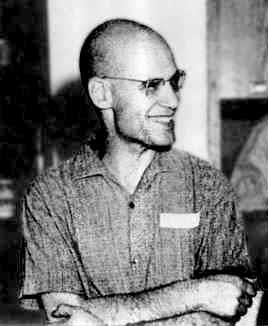
\includegraphics[scale=0.8]{images/groth}
\caption{Alexander Grothendieck.}
\end{center}
\end{figure}

\subsection{Introduction}
Affine varieties over a field $k$ correspond to commutative rings $R$ that satisfy the following properties:
\begin{enumerate}
	\item $R$ is a $k$-algebra;
	\item $R$ is finitely-generated as an algebra;
	\item $R$ is reduced.
\end{enumerate}
The coordinate ring of an affine variety has these properties. Further, one can construct an affine variety from a commutative ring with these properties.

The coordinate ring of a line $k[x]$ behaves similarly to $\mathbf{Z}$ or algebraic number fields such as $\mathbf{Z}[i]$. It was noticed in the nineteenth century that the theory of algebraic number fields was very similar to the theory of curves over finite fields. Hence, one wants algebraic geometry to include these things, so we don't want to require that $R$ is an algebra over a field. 

One might want to consider the localization of the ring of rational functions $k(x)$ at the ideal $(x)$. However, this is not finitely-generated as an algebra.

Further, one might want to intersect curves $y=x^2$ and $y=0$. Then, one considers the ring $k[x,y]/(y,x^2-y) \isomto k[x]/ (x^2)$. Classically, one replaces this with $k[x]/(x) = k$. However, when one does this, one loses information about the intersection. This replacement is the coordinate ring of a point, and while these curves intersect at a point, that point is really a ``double point.'' The ring $k[x]/(x^2)$ is two-dimensional, so it keeps track of the ``double point''; however, it has nilpotent elements.

One sees the benefit in abandoning these extra conditions. Hence, one wants to define some generalization of an affine variety that corresponds to commutative rings. We shall call these mysterious things ``affine schemes.''\index{affine scheme} However, to define them, one needs to look into the theory of sheaves.

\index{sheaf}Sheaves were introduced by Jean Leray circa 1950. Thereafter, Jean-Pierre Serre and Henri Cartan used them to study analytic varieties. Serre introduced sheaves to algebraic geometry in his famous ``Faisceaux Algébriques Cohérents'' of 1955.\footnote{FAC is a superb introduction to sheaf theory.}

Prior to the introduction of sheaves, people found all sorts of invariants in algebraic geometry. Take, for example, the \index{arithmetic genus}arithmetic genus, which didn't seem to depend on a surface's embedding in projective space. It was hard to define or compute, though: One of its definitions was
\begin{align*}
	p\textsubscript{a} = \binom{\mu_0-1}{2} - (\mu_0 - 4) \epsilon_0 + \frac{\epsilon_1}{2} - \epsilon_0+2t
\end{align*}
where these numbers are some rather strangely-defined invariants.\footnote{This was the definition for two dimensions. Good luck generalizing it.} With sheaves, the arithmetic genus of a surface is
\begin{align*}
	p\textsubscript{a} = \chi -1
\end{align*}
where the Euler characteristic $\chi$ is given by an alternating sum of dimensions of sheaf cohomology groups.

Another such invariant was the \defn{irregularity}\index{irregularity of a surface} of a surface. The irregularity was a weird thing that was related to the difference between the arithmetic and geometric genuses. However, with sheaves, it is, simply, the dimension of the first sheaf cohomology group of the structure sheaf. One extends this to higher dimensions by considering the dimension of higher sheaf cohomology groups. More generally, one defines the \defn{Hodge number}\index{Hodge number} 
\begin{align*}
	{\h}^{pq}(X) := \dim \HH^q(X,\Omega^p) 
\end{align*}
as the dimension of the $q$th homohology group of a sheaf of $p$-forms over a surface.

\begin{example}[Motivation]\label{}\text{}
Suppose $X$ is a topological space with an open set $U$. Let $\mathscr{F}(U)$ be the continuous functions from $U$ to $\mathbf{R}$. That is, $\mathscr{F}$ goes from open sets to abelian groups. One will call $\mathscr{F}$ a (pre)sheaf of abelian groups. 

If $V$ and $U$ are open sets and $V\subseteq U$, there is a restriction map
\begin{align*}
	\rho_{U}^V : \mathscr{F}(U)  \longrightarrow \mathscr{F}(V).
\end{align*}
Given open sets $W\subseteq V\subseteq U$, the restriction map $\rho$ makes
\[
\begin{tikzcd}
	\mathscr{F}(U)\ar[r,"\rho"] \ar[dr,"\rho", swap] &  \mathscr{F}(V)\ar[d,"\rho"] \\
						   & \mathscr{F}(W)
\end{tikzcd}
\]
commute. That is, $\rho_{U}^W = \rho_{V}^W \rho_{U}^V$. Further, $\rho_{U}^U$ is the identity.

A \defn{presheaf}\index{presheaf} of abelian groups is a map
\begin{align*}
	\mathscr{F} : \textrm{open subsets of $X$} \longrightarrow \textrm{abelian groups}
\end{align*}
together with restriction maps $\rho_{U}^V : \mathscr{F}(U) \longrightarrow  \mathscr{F}(V)$ for all open sets $U\subseteq V$ satisfying the above conditions. 
\end{example}

One can think of $\mathscr{F}$ as a contravariant functor from $\catn{Op}_X$ to $\catn{Ab}$. The objects of $\catn{Op}_X$ are open sets; further, there is $1$ morphism $U\longrightarrow V$ if $U\subseteq V$ and $0$ otherwise. One sees that $\mathscr{F}$ is assigning an abelian group to every open set and giving a map from the abelian group of $V$ to the abelian group of $U$ whenever $U\subseteq V$.

\begin{remark}
	This indicates that one can replace $\catn{Op}_X$ with another category and still define presheaves (and similarly for $\catn{Ab}$). Grothendieck did this to define \'etale cohomology.
\end{remark}

\begin{example}[Presheaves]\label{}\text{}
\begin{enumerate}
	\item Let $X$ be a smooth manifold. Let $\mathscr{F}(U)$ be the smooth vector fields on $U$. Not only is $\mathscr{F}$ a presheaf, $\mathscr{F}$ is a sheaf.
	\item Let $X$ be an affine variety. Let $\mathscr{F}(U)$ be the regular functions on $U$.
	\item Let $X$ be a Riemann surface. Let $\mathscr{F}(U)$ be the holomorphic functions on $U$. Riemann surfaces can be viewed as complex manifolds, smooth real manifolds, or topological manifolds. One gets different sheaves of functions from these perspectives.
	\item Let $\mathscr{F}(U) = A$ be a fixed abelian group. This is a presheaf.\footnote{This is not true for all definitions of ``presheaf.'' For example, Hartshorne adds the condition that $\mathscr{F}(\emptyset) = 0$.}
\end{enumerate}
\end{example}


Suppose $U$ is a union of open sets $U_\alpha$. A presheaf $\mathscr{F}$ is \defn{separated}\index{separated presheaf} if the image of $f$ in all $\rho_{U}^{U_\alpha}$ is $0$ implies $f=0$ for all $f\in \mathscr{F}(U)$. 

Suppose that $\mathscr{F}$ is separated. Suppose $f_\alpha,f_\beta\in \mathscr{F}(U_\beta)$ have the same image in $\mathscr{F}(U_\alpha\cap U_\beta)$. If one can find $f\in \mathscr{F}(U)$ with images $f_\alpha$ in $\mathscr{F}(U_\alpha)$, then $\mathscr{F}$ is a \defn{sheaf}\index{sheaf}.

\begin{example}[Presheaves that are not sheaves]\label{}\text{}
\begin{enumerate}
	\item Let $\mathscr{F}(U) = A$ for a fixed abelian group $A\ne 0$. A sheaf satisfies $\mathscr{F}(\emptyset) = 0$.
	\item Let
		\begin{align*}
			\mathscr{F}(U) = 
			 \begin{cases}
				 0&U=\emptyset\\
				 A&\textrm{otherwise.}
			\end{cases}
		\end{align*}
		Let $U = U_1\sqcup U_2$. Then $\mathscr{F}(U) =A$, but, if $\mathscr{F}$ were a sheaf, then $\mathscr{F}(U) =  \mathscr{F}(U_1)\times \mathscr{F}(U_2) = A\times A$.
\end{enumerate}

A presheaf $\mathscr{F}$ is a sheaf if the following sequence is exact:
\[
\begin{tikzcd}
	0 \ar[r] & \mathscr{F}(U) \ar[r] & \displaystyle\prod_\alpha  \mathscr{F}(U_\alpha) \ar[r, yshift = 0.5 ex] \ar[r, yshift = -0.5 ex] & \displaystyle\prod_{\alpha,\beta}  \mathscr{F}(U_\alpha\cap U_\beta).
\end{tikzcd}
\]
Note that 
\[
\begin{tikzcd}
	A\ar[r] &A\times A \ar[r, yshift = 0.5 ex] \ar[r, yshift = -0.5 ex] & 0 
\end{tikzcd}
\]
is not exact.
\end{example}

By the way, an element $s\in \mathscr{F}(U)$ is called a \defn{section}\index{section} and an element $s\in \mathscr{F}(X)$ is called a \defn{global section}\index{global section}.

\subsection{\'Etale spaces}
Sheaves seem to be an unnecessarily complicated and abstract way to describe functions on a space. Of course, this isn't the case.

\begin{example}[ ]\label{}\text{}
The points of the affine line $\mathbf{C}$ correspond to the maximal ideals of the ring $\mathbf{C}[x]$.\footnote{The point $\alpha\in \mathbf{C}$ corresponds to the maximal ideal $(x-\alpha)$.} Given $f\in \mathbf{C}[x]$, define
\begin{align*}
	D_f := \{\alpha : f(\alpha)\ne 0\}.
\end{align*}
Then, open sets have a basis $\{D_f\}$ in the Zariski topology. Further, the ring of regular functions of an open set is given as follows: 
\begin{align*}
	\mathscr{F}(D_f) = \{g/f^n: g\in \C[x]\}
\end{align*}

Let us replace $\mathbf{C}[x]$ with $\mathbf{Z}$. The maximal ideals of $\mathbf{Z}$ are given by
\begin{align*}
	\specmax\mathbf{Z} = \{(2),  (3),\hdots\}.
\end{align*}
This set is called the \defn{maximal spectrum}\index{maximal spectrum} of $\mathbf{Z}$. Given $f\in \mathbf{Z}$, define 
\begin{align*}
	D_f := \{\mathfrak{m}: f\notin  \mathfrak{m}\}.
\end{align*}
Then, one gets a basis of open sets $\{D_f\}$. Now, define
\begin{align*}
	\mathscr{F}(D_f) := \{ g/f^n : g\in \mathbf{Z}\}.
\end{align*}

One pretends that an integer is a function on the space $\specmax \mathbf{Z}$. One notes the difference, though: $f\in \C[x]$ has values in $\mathbf{C}$ at all points of $\mathbf{C} = \mathbf{C}[x]/(x-\alpha)$, but $f\in \mathbf{Z}$ has values in $\mathbf{Z}/(p)$, which varies as the point varies. Nevertheless, $\mathscr{F}$ satisfies the sheaf property.\footnote{This fact comes down to the fundamental theorem of arithmetic.}
\end{example}

Sheaves of sets behave similarly to sets; likewise, sheaves of abelian groups behave similarly to abelian groups. Hence, one can form a category of sheaves of sets and of sheaves of abelian groups. Given sheaves $\mathscr{F}$ and $\mathscr{G}$, one has a morphism by defining a morphism $\mathscr{F}(U) \longrightarrow \mathscr{G}(U)$ for all open sets $U$ that is compatible with the restriction map: Given open sets $V\subseteq U$,
\[
\begin{tikzcd}
	\mathscr{F}(U)\ar[d,"\rho", swap] \ar[r]&  \mathscr{G}(U)  \ar[d,"\rho"] \\
	\mathscr{F}(V) \ar[r]&  \mathscr{G}(V)
\end{tikzcd}
\]
commutes. Hence, sheaves comprise a category.

The category of sheaves of sets is a sort of weak model of set theory. It is called a \defn{topos}\index{topos}: One does set theory with sheaves over a topological space instead of sets.

Suppose
\[
\begin{tikzcd}
	0\ar[r]&A\ar[r]&B\ar[r]&C\ar[r]&0
\end{tikzcd}
\]
is an exact sequence of abelian groups. What this means is clear. Now, what does it mean for
\[
\begin{tikzcd}
        0\ar[r]&\mathscr{A}\ar[r]&\mathscr{B}\ar[r]&\mathscr{C}\ar[r]&0,
\end{tikzcd}
\]
a sequence of sheaves, to be exact? The obvious guess is that
\[
\begin{tikzcd}
	0\ar[r]&\mathscr{A}(U)\ar[r]&\mathscr{B}(U)\ar[r]&\mathscr{C}(U)\ar[r]&0
\end{tikzcd}
\]
is exact for all open sets $U$. This is wrong: While this is okay for saying that $\mathscr{A}\longrightarrow \mathscr{B}$ is injective, it is not for saying that $\mathscr{B} \longrightarrow \mathscr{C}$ is surjective.

\begin{example}[ ]\label{}\text{}
Let $X$ be a circle. Let $X_1=X$ and $X_2$ be a circle winding around $X$ twice. Let $\mathscr{F}_1(U)$ be the sections from $U$ to $X_1$ and $\mathscr{F}_2(U)$ be the sections from $U$ to $X_2$. These are sheaves. There is a natural surjective map from $X_2$ to $X_1$ (and a map from $X_1$ to $X$), whence one gets a natural map $\mathscr{F}_2\longrightarrow \mathscr{F}_1$. Note that $\mathscr{F}_2(X) \longrightarrow \mathscr{F}_1(X)$ is not surjective: $\mathscr{F}_1(X)$ is a point and $\mathscr{F}_2(X)$ is empty, since there are no continuous maps from $X$ to $X_2$ that are sections of it.

Hence, one has two different ways to talk about surjectivity depending on whether one looks at $X_2\longrightarrow X_1$ or $\mathscr{F}_2(X) \longrightarrow \mathscr{F}_1(X)$. These correspond to local and global notions respectively, and it turns out that one should work with a local definition. 
\end{example}

Suppose one has a continuous map from $A$ to $X$. One can construct a sheaf by letting $\mathscr{F}(U)$ be continuous sections from $U$ to $A$. Suppose further that one has a continuous map from $B$ to $X$. If $\mathscr{F}$ is the ``sheaf of $A$'' and $\mathscr{G}$ is the ``sheaf of $B$,'' a continuous map from $A$ to $B$ such that
\[
\begin{tikzcd}
	A \ar[d]\ar[r] &B\ar[dl]\\X
\end{tikzcd}
\]
commutes induces a map $\mathscr{F}\longrightarrow \mathscr{G}$. The map $\mathscr{F}(X) \longrightarrow \mathscr{G}(X)$ does not need to be surjective if $A\longrightarrow B$ is surjective.

\begin{problem}
	Does a sheaf $\mathscr{F}$ come from a map $A\longrightarrow X$ for some $A$?
\end{problem}

The answer is ``yes,'' even if one replaces ``sheaf'' with ``presheaf.'' Now, we shall construct the \index{\'etale space}\'etale space of the presheaf $\mathscr{F}$. 

Given a space $X$, we want to construct a space $A$ mapping to $X$ that has something to do with $\mathscr{F}$. First, given $x\in X$, we want to determine the fibre of $A$ above $x$. A point $p$ of the fibre is given by a section $f\in \mathscr{F}(U)$ for some open neighbourhood $U$ of $p$. One says that $f$ and $g$ are the same point of the fibre if the images of $f$ and $g$ in $V$ are the same for some small $V$ containing $p$. Thus, if one thinks of $\mathscr{F}$ as the continuous sections of something, then the fibre is, roughly, equivalence classes of sections.

Now, endow $A$ with a topology. A basis of open sets is given as follows: Suppose $f\in \mathscr{F}(U)$. For every $p\in U$, take the image of $f$ in the fibre above $p$. The union of these images is an open set. These open sets give a basis for the topology. One calls $A$ the \defn{\'etale space}\index{\'etale space} of $\mathscr{F}$. Note that a map $A\longrightarrow X$ is \defn{\'etale} if, for all $\alpha\in A$, there is a neighbourhood $V$ of $\alpha$ such that the map from $V$ to $\img X$ is a homeomorphism.

\subsection{Exactness and sheaves}
\begin{example}[ ]\label{}\text{}
Let $X=\mathbf{R}$ and let $\mathscr{F}$ be the sheaf of smooth functions, so $\mathscr{F}(U)$ comprises the smooth functions on $U$. One can think about the fibre above $0$ as germs of smooth functions at $0$. Let $A = \Et ( \mathscr{F})$ be the \'etale space of $\mathscr{F}$. 

Note that $A$ is not Hausdorff: Consider the fibres $f=0$ and $g$, where $g$ is a smooth function that is $0$ to the left of $0$ and has infinitely many bumps to the right. 
One sees that $f$ and $g$ are distinct points of the fibre above $0$ since there are no open neighbourhoods of $0$ in which they are the same. However, any open neighbourhoods of $f$ and $g$ have a point in common.

If $\mathscr{G}$ is the sheaf of analytic functions, then $\Et(\mathscr{G})$ is Hausdorff.
\end{example}

From any presheaf $\mathscr{F}$, one gets an \'etale space. From any \'etale space, one gets a sheaf of sections $\mathscr{F}\sh$. The sheaf $\mathscr{F}\sh$ is called the \defn{sheafification}\index{sheafification} of the presheaf $\mathscr{F}$. Note the following properties:
\begin{enumerate}
	\item If $\mathscr{F}$ is a presheaf and $\mathscr{G}$ is a sheaf and one has a map $\mathscr{F}\longrightarrow \mathscr{G}$, one has a unique sheaf morphism such that
		\[
		\begin{tikzcd}
			\mathscr{F} \ar[r] \ar[d] & \mathscr{G}\\
			\mathscr{F}\sh \ar[ur, dashed]
		\end{tikzcd}
		\]
		commutes.
	\item If $\mathscr{F}$ is a sheaf, then $\mathscr{F}\longrightarrow \mathscr{F}\sh$ is an isomorphism. 
	\item If $A\longrightarrow X$ is \'etale and $\mathscr{F}$ is the sheaf of sections, then
		\begin{align*}
			\Et ( \mathscr{F} ) \isomto A.
		\end{align*}
\end{enumerate}

Thus, sheaves over $X$ are sort of equivalent to \'etale spaces $A\longrightarrow X$.\footnote{Sheaves are called ``sheaves'' because the \'etale space of a sheaf is the union of its fibres (stalks). Note that the definition of ``sheaf'' is ``a bundle of grain stalks laid lengthwise and tied together after reaping.''} In particular, a morphism of sheaves $\mathscr{F}\longrightarrow \mathscr{G}$ is an isomorphism if and only if the corresponding morphism of \'etale spaces is an isomorphism if and only if it is an isomorphism for all stalks. Let us digress to clarify some useful definitions.

 \begin{definition}[ ]\label{}\text{}
Let $\mathscr{F}$ be a presheaf on $X$. Let $x\in X$. The \defn{stalk}\index{stalk} of $\mathscr{F}$ at $x$ is the set
\begin{align*}
	\mathscr{F}_x := \varinjlim_{U\ni x} \mathscr{F}(U).
\end{align*}
Equivalently,
\begin{align*}
	\mathscr{F}_x = \{(U,s) : U\ni x, s\in  \mathscr{F}(U)\} / \sim
\end{align*}
where $(U_1,s_1)\sim(U_2,s_2) $ if and only if there exists an open set $U_3 \subset U_1\cap U_2$ with $x\in U_3$ and $s_1\big |_{U_3} = s_2\big |_{U_3}$.
\end{definition}

\begin{definition}[ ]\label{}\text{}
The \defn{germ}\index{germ} of $s\in \mathscr{F}(U)$ at a point $x$ is the equivalence class of $(s,U) \in  \mathscr{F}_x$.
\end{definition}

\begin{example}[Sheafification]\label{}\text{}
Let $\mathscr{F}$ be the constant presheaf; that is,
\begin{align*}
	\mathscr{F}(U) := A
\end{align*}
for some fixed abelian group $A$. The fibre at each point is $A$. Hence, one sees that the \'etale space is $X\times A \longrightarrow X$ where $A$ has the discrete topology. Hence, $\mathscr{F}\sh(U)$ is continuous maps $U\longrightarrow A$. Since $A$ has the discrete topology, $\mathscr{F}\sh(U)=A$ if $U$ is connected and nonempty.\footnote{Apparently, the connectedness of the empty set is contested.} Further, $\mathscr{F}\sh(\emptyset ) = 0$. If $U$ has two open components, then $\mathscr{F}\sh(U) = A\times A$. 
\end{example}

A sequence of sheaves on $X$
\[
\begin{tikzcd}
	\mathscr{F} \ar[r] &\mathscr{G}\ar[r] &\mathscr{H}
\end{tikzcd}
\]
is exact if it is exact on the fibres (stalks). Similarly, a morphism of sheaves $\mathscr{F}\longrightarrow \mathscr{G}$ is injective/surjective if it is on the fibres (stalks).

\begin{example}[Skyscraper sheaf]\label{}\text{}
Fix $x\in X$ and an abelian group $A$. Define
\begin{align*}
	\mathscr{F}(U) := 
	 \begin{cases}
		 A & x\in U\\
		 0&\textrm{otherwise.}
	\end{cases}
\end{align*}
This is a sheaf called the \defn{skyscraper sheaf}\index{skyscraper sheaf} of $\mathscr{F}$ at $x$. Let $\mathscr{G}$ be the sheaf of smooth functions on $\mathbf{R}$. Given $\alpha\in \mathbf{R}$, one gets a map 
\[
\begin{tikzcd}
	0\ar[r] & \mathscr{G}\ar[r, "\times \alpha"] &\mathscr{G}.
\end{tikzcd}
\]
At all nonzero points, the corresponding map of fibres is an isomorphism, so the second arrow is an isomorphism except at $0$. One sees that
\[
\begin{tikzcd}
	0\ar[r] &\mathscr{G}\ar[r,"\times \alpha"] &\mathscr{G}\ar[r] &\mathscr{F}\ar[r] &0
\end{tikzcd}
\]
is exact where $\alpha = 0$ and $A=\mathbf{R}$, since, for nonzero $\alpha$, one gets the sequence of fibres
\[
\begin{tikzcd}
	0 \ar[r] & B\ar[r, "\times \alpha"] & B\ar[r] &0
\end{tikzcd}
\]
where $B$ is a space of all germs of functions at $0$ and the second arrow is an isomorphism, and, for $\alpha = 0$, one gets
\[
\begin{tikzcd}
	0\ar[r] & B\ar[r,"\times\alpha"] & B\ar[r] & \mathbf{R}\ar[r] & 0.
\end{tikzcd}
\]
\end{example}

\begin{example}[ ]\label{}\text{}
Consider the sequence
\[
\begin{tikzcd}
	0 \ar[r] & 2\pi i \mathbf{Z} \ar[r] & \textrm{holomorphic functions} \ar[r, "\exp"] &\textrm{holomorphic functions $\ne 0$} \ar[r] & 0
\end{tikzcd}
\]
where $2\pi i \mathbf{Z}$ is, really, the constant sheaf of $2\pi i \mathbf{Z}$ (and the rest of the things are sheaves, too).\footnote{``Holomorphic functions $\ne 0$'' means ``(the sheaf of) holomorphic functions that do not vanish anywhere.''} This is an exact sequence of sheaves because it is exact on fibres (the third arrow is surjective since one can take $\log$ in the neighbourhood of a point). However, it is not exact on sections of open sets: Take $U = \mathbf{C}-\{0\}$ and let $f(z)=z$ be the nonzero holomorphic function. Then, there must be a function $g$ such that $\exp g = z$ at all points. One recalls that this doesn't work: $\log$ is not holomorphic.
\end{example}

\subsection{$f_*$ and $f^{-1}$}
Suppose $f:X\longrightarrow Y$ is a continuous map of topological spaces. Let $\catn{Sh}_X$ be the category of sheaves of abelian groups on $X$. We shall define functors $f_* : \catn{Sh}_X \longrightarrow \catn{Sh}_Y$ and $f^{-1} : \catn{Sh}_Y \longrightarrow \catn{Sh}_X$.

Recall that a sheaf $\mathscr{F}$ on $X$ can be viewed as a map from the open sets of $X$ to abelian groups or as an \'etale space over $X$.

If $U$ is an open subset of $Y$, then
\begin{align*}
	f_*(\mathscr{F}) (U) :=  \mathscr{F}(f^{-1}(U))
\end{align*}
where $f^{-1}(U)$ is the preimage of $U$ under $f$.

\begin{example}[ ]\label{}\text{}
Let $Y$ be a point. Let $\mathscr{F}$ be a sheaf on $X$. The space $Y$ has $1$ nonempty open set, so a sheaf on $Y$ is a group. Therefore,
\begin{align*}
	f_*(\mathscr{F}) (Y) =  \mathscr{F}(X)
\end{align*}
comprises the global sections of $\mathscr{F}$.
\end{example}

One sees that $f_*$ does not preserve surjectivity: If $\mathscr{F}_1\longrightarrow \mathscr{F}_2$ is a surjective morphism of sheaves, then $f_*(\mathscr{F}_1)\longrightarrow f_*(\mathscr{F}_2)$ does not need to be surjective.

Suppose
\[
\begin{tikzcd}
	0 \ar[r] &\mathscr{A} \ar[r] &\mathscr{B} \ar[r] &\mathscr{C}\ar[r]&0
\end{tikzcd}
\]
is an exact sequence of sheaves on $X$. Then
\[
\begin{tikzcd}
	0 \ar[r]&f_*(\mathscr{A}) \ar[r] &f_*(\mathscr{B}) \ar[r] &f_*(\mathscr{C})
\end{tikzcd}
\]
is exact. 

Suppose $p$ is a point of $Y$. The elements of the fibre of $f_*(\mathscr{B})$ above $p$ are given by elements of $f_*(\mathscr{B})(U)$ where $U\ni p$; this set is given by $\mathscr{F}(f^{-1}(U))$ where $f^{-1}(U)$ denotes the premiage. Given an exact sequence sequence of sheaves
\[
\begin{tikzcd}
	 0 \ar[r] &\mathscr{A} \ar[r] &\mathscr{B} \ar[r] &\mathscr{C}\ar[r]&0
\end{tikzcd}
\]
and an element in $f_*(\mathscr{B})$ that is in the kernel of the third arrow, it must be the image of something in $f_*(\mathscr{A})$. Thus, the resulting sequence is exact.

Let $\mathscr{G}$ be a sheaf on $Y$. The sheaf $\mathscr{G}$ corresponds to an \'etale space $B$ over $Y$. so there is a local homeomorphism $B\longrightarrow Y$. One has a pullback square
\[
\begin{tikzcd}
	B\times_Y X \ar[r] \ar[d] & B\ar[d]\\
	X \ar[r] & Y
\end{tikzcd}
\]
whose kernel is the subset of $B\times_Y X$ consisting of points that have the same image in $Y$. Alternatively, if $p$ is a point in $X$, then the fibre above $p$ of $B\times Y X$ is the same as the fibre above $f(p)$ of $B$. The check that $B$ is \'etale over $Y$ implies that $B\times_Y X$ is \'etale over $X$ is straightforward, so $B\times_Y X$ gives a sheaf. One defines $f^{-1}(\mathscr{G})$ to be the sheaf of the \'etale space $B\times_Y X\longrightarrow X$.

\begin{remark}
	The functor $f^{-1}$ preserves exactness.
\end{remark}

\begin{example}[ ]\label{}\text{}
Suppose $X\subseteq Y$. If $\mathscr{G}$ is a sheaf on $Y$, then $f^{-1}(\mathscr{G})$ can be thought of as the restriction of $\mathscr{G}$ to $X$. The fibre of $f^{-1}(\mathscr{G})$ at $p\in X$ is the fibre of $\mathscr{G}$ at $p\in Y$.
\end{example}

Notice that $f^{-1}$ is left adjoint to $f_*$: Suppose $\mathscr{F}$ is a sheaf on $X$ and $\mathscr{G}$ is a sheaf on $Y$. Then $f^{-1}(\mathscr{G})$ is a sheaf on $X$ and $f_*(\mathscr{F})$ is a sheaf on $Y$. One has maps
\[
\begin{tikzcd}
	f^{-1}(\mathscr{G}) \ar[d]& \mathscr{G}\ar[d]\\
	\mathscr{F} & f_*(\mathscr{F}).
\end{tikzcd}
\]
Informally, adjointness means that these maps are the same in some sense. One might see this via the fact that maps $f^{-1}(\mathscr{G})\longrightarrow \mathscr{F}$ and $\mathscr{G}\longrightarrow f_*(\mathscr{F})$ are somehow the same as collections of maps $\mathscr{G}(V) \longrightarrow \mathscr{F}(U)$ whenever one has open sets $U\subseteq X$ and $V\subseteq Y$ with $f(U)\subseteq V$; these maps must be compatible with the restriction maps.

If $F$ is left adjoint to $G$, then $F$ preserves right exactness and $G$ preserves left exactness. Since $f^{-1}$ is left adjoint to $f_*$, one sees that $f_*$ is left exact (as we showed) and $f^{-1}$ is right exact (as we showed). Note, however, that we showed that $f^{-1}$ is exact (that is, it is also left exact).

\subsection{Definition of a scheme}
Alexander Grothendieck introduced schemes in the 1950s. At this time, mathematicians such as Weil, Serre, Chevalley, and Grothendieck were experimenting with the foundations of algebraic geometry and looking at potential generalizations of algebraic varieties. The figure below illustrates generalizations of projective varieties.
\begin{center}
\begin{tikzpicture}[level 1/.style = {sibling distance = 5 cm}, level 4/.style = {sibling distance = 5 cm}]
	\node {Projective variety}[edge from parent fork down]
		child { node {Abstract variety\index{abstract variety} (Weil)}
			child {node {Scheme (Grothendieck)\index{scheme}}
				child {node {Locally ringed space\index{locally ringed space}}
					child {node{Locally ringed topos\index{locally ringed topos}}}}
				child {node {Algebraic space\index{algebraic space}}
					child {node{Stack\index{stack}}}}
				}
		};
\end{tikzpicture}
\end{center}

Smooth manifolds, complex manifolds, and topological maniforlds are examples of locally ringed spaces.
A quotation of János Kollár that is found in \underline{The Princeton Companion to Mathematics} sums up the theory of stacks: 
\begin{center}
	\small The study of stacks is strongly recommended to people who would have been flagellants in earlier times. (367)
\end{center}

\begin{definition}[ ]\label{}\text{}
A \defn{scheme}\index{scheme} is a \index{locally ringed space}locally ringed space that is locally isomorphic to an \index{affine scheme}affine scheme.
\end{definition}

\begin{definition}[ ]\label{}\text{}
A \defn{ringed space}\index{ringed space} is a space $X$ together with a sheaf of rings.
\end{definition}

\begin{example}[Ringed space]\label{}\text{}
	A smooth manifold with the sheaf of smooth functions is a ringed space.
\end{example}

\begin{definition}[ ]\label{}\text{}
A \defn{locally ringed space}\index{locally ringed space} is a ringed space in which all stalks are local rings.
\end{definition}

\begin{remark}
	The maximal ideal corresponding to a stalk sort of corresponds to functions that vanish at the point.
\end{remark}

\begin{example}[Ringed space that isn't locally ringed]\label{}\text{}
Let $X$ be a topological space. Let $\mathscr{O}$ be a presheaf on $X$ given by $\mathscr{O}(U) := R$ for a fixed ring $R$. Then, $\mathscr{O}\sh(U)$ comprises functions $U\longrightarrow R$ where one gives $R$ the discrete topology. The local ring at $p\in X$ is isomorphic to $R$; hence, if $R$ is not a local ring, the corresponding ringed space is not locally ringed. 
\end{example}

\begin{definition}[ ]\label{}\text{}
An \defn{affine scheme}\index{affine scheme} is isomorphic to the spectrum $\Spec R$ of a ring $R$. The spectrum $\Spec R$ is a locally ringed space whose points are the prime ideals of $R$ and whose topology is given by a basis of open sets
\begin{align*}
	U_r = \{\mathfrak{p} \textrm{ prime}: \mathfrak{p}\not\ni r\}
\end{align*}
for $r\in R$; the sheaf of $\Spec R$ is given by
\begin{align*}
	\mathscr{O}(U_r) := R[r ^{-1}].
\end{align*}
\end{definition}

\begin{remark}
	One needs to define the sheaf on only the open sets $U_r$. Open sets that are not of this form tend to be unimportant and the action of the sheaf on the basis determines everything. By the way, it is not trivial that $\mathscr{O}$ is a sheaf.
\end{remark}

\begin{example}[ ]\label{}\text{}
\begin{enumerate}
	\item Let $R$ be a field. Then, $\Spec R$ has $1$ point $0$ and $\mathscr{O}(0)= R$.
	\item Let $R=\mathbf{Z}$. Then, the points of $\Spec R$ are $(0),  (2),  (3),\hdots$. One sees that $U_r$ is either $\emptyset$ or $\Spec R$ minus a finite number of nonzero primes.\footnote{Not only is $\Spec R$ not necessarily Hausdorff, its points don't need to be closed: $(0)$ is not closed.} Also,
		 \begin{align*}
		 	\mathscr{O}(U_r) = \{ m/r^k\}.
		 \end{align*}
		 Further, the local ring at $(0)$ is $\mathbf{Q}$ and the local ring at $(p)$ is
		 \begin{align*}
		 	\mathbf{Z}_{(p)} := \{ m/n:p\nmid n\}.
		 \end{align*}
	 \item Let $R=\mathbf{C}[z]$. Then, $\Spec R$ has points $(0)$ and $(z-\alpha)$ for $\alpha\in \mathbf{C}$. One sees that 
\begin{align*}
	U_f = \{ (z-\alpha) : f (\alpha)\ne 0\}
\end{align*}
is either $\emptyset$ or $\Spec R$ minus a finite number of points. Also, $\mathscr{O}(U_f)$ consists of rational functions $g/f^k$ that have no poles on $D_f$. Further, the local ring at $(0)$ is $\mathbf{C}(z)$ and the local ring at $(z-\alpha)$ comprises rational functions with no poles at $\alpha$.
\end{enumerate}
\end{example}

Let us see why the locally ringed space $\Spec R$ is called the ``spectrum.'' First, the spectrum of an atom is related to the spectrum of a linear operator on a Hilbert space. 

Second, the eigenvalues of a matrix $A$ correspond to the maximal ideals of $\mathbf{C}[A]\isomto \mathbf{C}[z]/(\mu(z))$ where $\mu$ is the minimal polynomial of $A$. 

Now, let $X$ be compact and Hausdorff. Let $R=C(X)$ be the ring of continuous real-valued functions on $X$. Then, the points of $X$ correspond to the (closed) maximal ideals of $R$ and the topology is given by $U_f$ (the open set of maximal ideals that do not contain $f$) for all $f$.

Hence, one says that the maximal ideals of a commutative ring form a topological space defined in this way. An obvious question arises:
\begin{center}
	\small Why prime ideals instead of maximal ideals, then?
\end{center}
Maximal ideals work just fine in specific settings, but not in general: Suppose $f:R\longrightarrow S$ is a homomorphism of rings. One wants to define a map $\Spec S \longrightarrow \Spec R$ given by $\mathfrak{m} \longmapsto f^{-1}(\mathfrak{m})$. However, $f^{-1}(\mathfrak{m})$ does not need to be maximal.\footnote{Let $f:\mathbf{Z} \longrightarrow \mathbf{Q}$ be the inclusion. Then $\mathfrak{m}=(0)$ is maximal in $\mathbf{Q}$ since $\mathbf{Q}$ is a field, but $f^{-1}(\mathfrak{m}) = (0)$ is not maximal in $\mathbf{Z}$ since $\mathbf{Z}$ is not a field.}

An $R$-ideal $\mathfrak{m}$ is maximal if and only if $R/\mathfrak{m}$ is a field. One sees that $R/f^{-1}(\mathfrak{m})$ is a subring of the field $S/\mathfrak{m}$, so one finds that $R/f^{-1}(\mathfrak{m})$ is an integral domain, but not necessarily a field. Recall that an $R$-ideal $\mathfrak{p}$ is prime if and only if $R/\mathfrak{p}$ is an integral domain. Therefore, if $\mathfrak{p}$ is a prime ideal, then $f^{-1}(\mathfrak{p})$ is prime. This is why Grothendieck considered prime ideals instead of maximal ideals.

\subsection{$\Spec \C[x,y]$ and $\Spec \Z[x]$}
Consider $\C[x,y]$.\footnote{One can consider $\Omega[x,y]$ for any algebraically closed $\Omega$.} There are three types of prime ideals:
\begin{enumerate}
	\item For any $(\alpha,\beta)\in  \mathbf{C}^2$, the maximal ideal $(x-\alpha,y-\beta)$ is prime;
	\item If $f(x,y)$ is irreducible, then $(f(x,y))$ is prime; 
	\item $(0)$.
\end{enumerate}
The local ring at $(0)$ is $\mathbf{C}(x,y)$. The local ring at $(x-\alpha, y-\beta)$ consists of rational functions whose denominators are nonzero at $(\alpha,\beta)$. The local ring at $\mathfrak{p} = (f(x,y))$ comprises all rational functions whose denominators are not divisible by $f$ (rational functions that are regular at almost all points).

\begin{definition}[ ]\label{}
The ring $R$ is a \defn{discrete valuation ring}\index{discrete valuation ring} if it is a PID that has a unique nonzero maximal ideal $\mathfrak{m}(R)$. The field $R/\mathfrak{m}(R)$ is the \defn{residue field}\index{residue field} of $R$. 
\end{definition}

\begin{remark}
The localization $\mathbf{C}[x,y]_\mathfrak{p}$ is a discrete valuation ring. Therefore, every element in the localization can be written as a power of $f$ times a unit.	
\end{remark}

Now, let $R$ be a discrete valuation ring (for example, $\mathbf{Z}_{(2)}$). One sees that $\mathfrak{m}(R) =  (2) $. The other ideals of $R$ are $(0)$ and $(2^n)$.\footnote{Note that the ideal $(0)$ is prime, not maximal, and $(2^n)$ is neither prime nor maxmial.} Hence, $\Spec R$ has two points.\footnote{The space $\Spec R$ is the \defn{Sierpi\'nski space}\index{Sierpi\'nski space}; that is, it is the topological space with two points, of which only one is closed.} The local ring at $(2)$ is $R$ and the stalk at $(0)$ is the field of fractions of $R$ (that is, $\mathbf{Q}$).

Now, let us consider $\Spec \mathbf{Z}[x] $. There is a ring homomorphism $\mathbf{Z}\longrightarrow \mathbf{Z}[x]$, so there is a map $\Spec \mathbf{Z}[x] \longrightarrow \Spec \mathbf{Z}$.\footnote{Recall that the generic point $(0)$ in $\Spec \mathbf{Z}$ contains all of the other points of $\Spec\mathbf{Z}$ in its closure.} The fibre above $(2)$ is $\Spec\mathbf{F}_{2}[x]$, which is the closure of the generic point $(2)$. The same thing happens for all prime numbers $p$. For the fibre above $(0)$, one looks at ideals whose intersection with $\mathbf{Z}$ is $(0)$, so one tensors with $\mathbf{Q}$ to get a map
\begin{align*}
	\mathbf{Z}[x]/\mathfrak{p}\tensor \mathbf{Q}\longrightarrow \mathbf{Q}(\alpha). 
\end{align*}
The image of $x$ under this map is some algebraic integer. The corresponding prime ideals shall be of the form $(f(x))$ where $f(x) $ is irreducible in $\mathbf{Z}[x]$. These prime ideals corresponding to irreducibles in $\mathbf{Z}[x]$, essentially, comprise $\Spec \mathbf{Q}[x]$. Thus, the closure of the generic point (the fibre above $(0)$) consists of $(x),  (x+1), (x+2),\hdots,  (x^2+1),\hdots$. These points correspond to algebraic numbers up to the action of $\Gal (\overline{\mathbf{Q}}/\mathbf{Q})$.

However, this isn't what $\Spec \mathbf{Z}[x]$ looks like. One thinks about $\Spec \mathbf{Z}[x]$ as a surface with points, vertical lines, and horizontal lines that illuminate algebraic number theory happening when they intersect.\footnote{See \url{https://youtu.be/WirufRI1_Uo?t=957}.} 

The local ring at $(2,x)$ consists of rational functions whose denominator has an odd constant term. The local ring at $(2)$ consists of rational functions whose denominator has an odd coefficient. The local ring at $(0)$ is $\mathbf{Q}(x)$.

\subsection{More examples of $\Spec R$}
\begin{example}[ ]\label{}\text{}
We have seen that $\Spec \mathbf{C}[x]$ looks like $\mathbf{C}$ with a generic point corresponding to the ideal $(0)$. This is not the case for $\mathbf{R}[x]$: While polynomials of the form $x-\alpha$ are irreducible, polynomials $x^2 + ax + b$ with two complex conjugate roots $\beta\pm \gamma i$ are also irreducible. Hence, one should also add in points that correspond to pairs of real numbers. Thus, $\Spec \mathbf{R}[x]$ consists of the orbits of $\mathbf{C}$ under complex conjugation---under $\Gal(\mathbf{C}/\mathbf{R})$---plus a generic point.
\end{example}

\begin{example}[ ]\label{}\text{}
Consider the ring of Gaussian integers $\mathbf{Z}[i]$. The principal ideal domain $\mathbf{Z}[i]$ has three flavours of prime ideals. To determine them, one takes a prime ideal in $\mathbf{Z}$ and figures out how it splits in $\mathbf{Z}[i]$. Observe how the following prime numbers factorize in $\mathbf{Z}[i]$:
\begin{align*}
	2 &= -i (1+i)^2;\\ 
	3 &= 3;\\
	5 &= (2+i) (2-i).
\end{align*}
The first case is unique to $2$; the second case happens for all $p\equiv 3\pmod 4$; and the third case happens for all $p\equiv 1\pmod 4$.

There is a map $\mathbf{Z}\longrightarrow \mathbf{Z}[i]$, so there is a map $\Spec \mathbf{Z}[i]\longrightarrow \Spec \mathbf{Z}$. The fibre above $(2)$ is $(1+i)$; the fibre above $(3)$ is $(3)$; and the fibre above $(5)$ is $\{(2+i),  (2-i)\}$. Similarly, the fibre above $(13)$ is $\{(3+2i),  (3-2i)\}$. One can think of the generic point $(0)$ as a curve that goes through all of these points. One might see that $\Spec \mathbf{Z}$ is similar to an affine line.\footnote{Note that $\mathbf{Z}[i]$ is a PID.}
\end{example}

\begin{remark}
	Given a geometric object (a ringed space) $X$, the \defn{Picard group}\index{Picard group} $\Pic X$ is the group of line bundles on $X$.\footnote{``Roughly speaking, a line bundle is a way of assigning a $1$-dimensional vector space to each point.''} Given an algebraic number field $K$, the \defn{ideal class group}\index{ideal class group} $\Cl_K$ of $K$---the group of fractional ideals modulo principal fractional ideals---correspond to a Picard group in some way.
\end{remark}

\begin{example}[ ]\label{}\text{}
Let us consider the spectrum of the localization $\C[x,y]_{(x,y)}$. First, $(0)$ is the generic point of $\Spec \C[x,y]_{(x,y)}$. Second, $(x,y)$ is the maximal ideal of this localization, so it gives a closed point. Further, one has points $(f(x,y))$ for $f(x,y)=0$. If one draws the spectra of $\mathbf{C}[x,y]$ and the localization we are considering, one notices that the latter looks like a magnification of the former at one point.
\end{example}

\begin{problem}
	What is $\Spec \text{}(0)$?
\end{problem}

The points of $\Spec R$ are the prime ideals of $R$. However, $(0)$ is not an integral domain, and it is its only ideal, so $\Spec \text{}(0)$ is empty. It has one open set, namely $\emptyset$. One defines the structure sheaf on $\Spec R$ by $\mathscr{O}(\emptyset) :=  (0)$.

\begin{example}[$\Spec (R\times S)$]
	The prime ideals of $R\times S$ are homomorphisms to integral domains. Either $S$ maps to $(0)$ or $R$ maps to $(0)$, so the primes of $R\times S$ are the primes of $R$ with the primes of $S$. It follows that $\Spec (R\times S)$ is a disjoint union $\Spec R\times \Spec S$. The corresponding structure sheaf is defined in the obvious way.
\end{example}

\subsection{Localization}
Suppose $R$ is a commutative ring and $S$ is a multiplicative subset of $R$. Suppose further that one wants to invert all elements of $S$. We shall construct a ring $R[S^{-1}]$ such that there is a universal homomorphism $R\longrightarrow R[S^{-1}]$ under which the image of $S$ consists of invertible elements. One takes
\begin{align*}
	R[S^{-1}] := \frac{R[t_1,t_2,\hdots]}{(s_1t_1-1,s_2t_2-1,\hdots)}.
\end{align*}

Let's determine the kernel $I$ of the map $R\longrightarrow R[S^{-1}]$. If $rs=0$ for some $s\in S$, then $r\in I$. Define
\begin{align*}
	I := \{r\in R: rs=0\textrm{ for some $s\in S$}\}.
\end{align*}
One can check that $I$ is an ideal. Further, $I$ is the kernel of $R\longrightarrow R[S^{-1}]$.

First, one assumes that $S$ has no zero divisors and copies the construction of $\mathbf{Q}$ from $\mathbf{Z}$: One sees that
\begin{align*}
	R[S^{-1}] = \left\{ (r,s) =  \frac{r}{s} : r\in R, s\in S \right\}/\sim 
\end{align*}
where $r_1/s_1 \sim r_2/s_2$ if and only if $r_1s_2 = r_2s_1$. Then, one defines 
\begin{align*}
	\frac{r_1}{s_1}+\frac{r_2}{s_2} &:= \frac{r_1s_2+r_2s_1}{s_1s_2};\\
	\frac{r_1}{s_1}\cdot\frac{r_2}{s_2}&:= \frac{r_1r_2}{s_1s_2}.
\end{align*}
The checks that $\sim$ is an equivalence relation and that these operations well-define a ring are relatively mundane, except for checking that $\sim$ is transitive: Suppose 
\begin{align*}
	\frac{r_1}{s_1}&\sim \frac{r_2}{s_2};\\
	\frac{r_2}{s_2}&\sim \frac{r_3}{s_3}.
\end{align*}
Then, $r_1s_2=r_2s_1$ and $r_2s_3=r_3s_2$. These equations imply $r_1s_2s_3=r_3s_2s_1$, so
\begin{align*}
	s_2(r_1s_3-r_3s_1)=0.
\end{align*}
Therefore, $r_1s_3=r_3s_1$ and $r_1/s_1\sim r_3/s_3$ if $s_2$ is not a zero divisor.

Now, suppose $S$ has zero divisors. Then, replace $R$ by $R/I$. The image of $S$ in $R/I$ has no zero divisors, so one can form $R/I[S^{-1}]$. One defines $R[S^{-1}]$ to be this ring. 

There is a one-step construction: Define
\begin{align*}
\frac{r_1}{s_1}\sim \frac{r_2}{s_2}	
\end{align*}
if $(r_1s_2-r_2s_1)s=0$ for some $s$. The construction above, however, is more intuitive and gives a clearer picture of things.

Now, suppose $S$ is the complement of a prime ideal $\mathfrak{p}$.\footnote{Exercise: Show that $S$ is multiplicative.} One writes
\begin{align*}
	R[S^{-1}] = R_{\mathfrak{p}}.
\end{align*}
This is the \defn{localization}\index{localization} of $R$ at $\mathfrak{p}$.

\begin{remark}
	If $R=\mathbf{C}[x]$, the dimension of the spectrum of $R/(0)$ is $1$ and that of $R_{(0)}$ is $0$. Further, the dimension of the spectrum of $R/(x-\alpha)$ is $0$ and that of $R_{(x-\alpha) }$ is $1$.

	If $R=\mathbf{C}[x,y]$, the dimension of the spectrum of $R/(0)$ is $2$ and that of $R_{(0)}$ is $0$. Furthermore, the dimensions of the spectra of $R/(f)$ and $R_{(f)}$ are $1$. Lastly, the dimension of the spectrum of $R/(x-\alpha, y-\beta)$ is $0$ and that of $R_{(x-\alpha,y-\beta)}$ is $2$. 
\end{remark}

\begin{remark}
	Taking $R/\mathfrak{p}$ makes $\mathfrak{p}$ minimal and taking $R_{\mathfrak{p}}$ makes $\mathfrak{p}$ maximal.
\end{remark}
\subsection{$\Spec R$ is a locally ringed space}
\subsection{Morphisms of affine schemes}
\subsection{Gluing schemes}
\subsection{$\Proj S$}
\subsection{The functor of points}
\subsection{Irreducible, reduced, integral, connected}
\subsection{Quasicompact, Noetherian}
\subsection{Morphisms of finite type}
\subsection{Finite, quasifinite}
\subsection{Immersions}
\subsection{Products}
\subsection{Groups schemes}
\subsection{Separated morphisms}
\subsection{Valuation rings}
\subsection{Valuations and separation}
\subsection{Proper morphisms}
\subsection{Proper morphisms and valuations}
\subsection{Abstract and projective varieties}
\subsection{Quasicoherent sheaves}
\subsection{Examples of quasicoherent sheaves}
\subsection{Invertible sheaves over the projective line}
\subsection{$f^*$ and $f_*$}
\subsection{Coherent sheaves}
\subsection{The line bundles $\mathscr O(n)$ on projective space}
\subsection{Vector bundles on the projective line}
\subsection{Coherent sheaves on projective space}
\subsection{Divisors on a Riemann surface}
\subsection{Weil and Cartier divisors}
\subsection{Comparison of Weil and Cartier divisors}
\subsection{Comparison of Cartier divisors and $\Pic$}
\subsection{Divisors and Dedekind domains}
\subsection{Examples of $\Pic X$}
\subsection{Morphisms to projective space}
\subsection{Very ample sheaves}
\subsection{Linear systems}
\subsection{$\Proj S$}
\subsection{Blowing up schemes}
\subsection{Differential operators}
\subsection{Cotangent bundle}
\subsection{The canonical sheaf}


\section{The Riemann--Roch theorem}
\subsection{Introduction}
\subsection{Genus $0$}
\subsection{Genus $1$}
\subsection{Structure of genus-$1$ curves}
\subsection{Genus-$2$ curves}
\subsection{Genus-$3$ curves}
\subsection{Plane curves}
\subsection{Proof of the Riemann--Roch theorem}


\section{The Weil conjectures}

\begin{figure}
	\begin{center}
		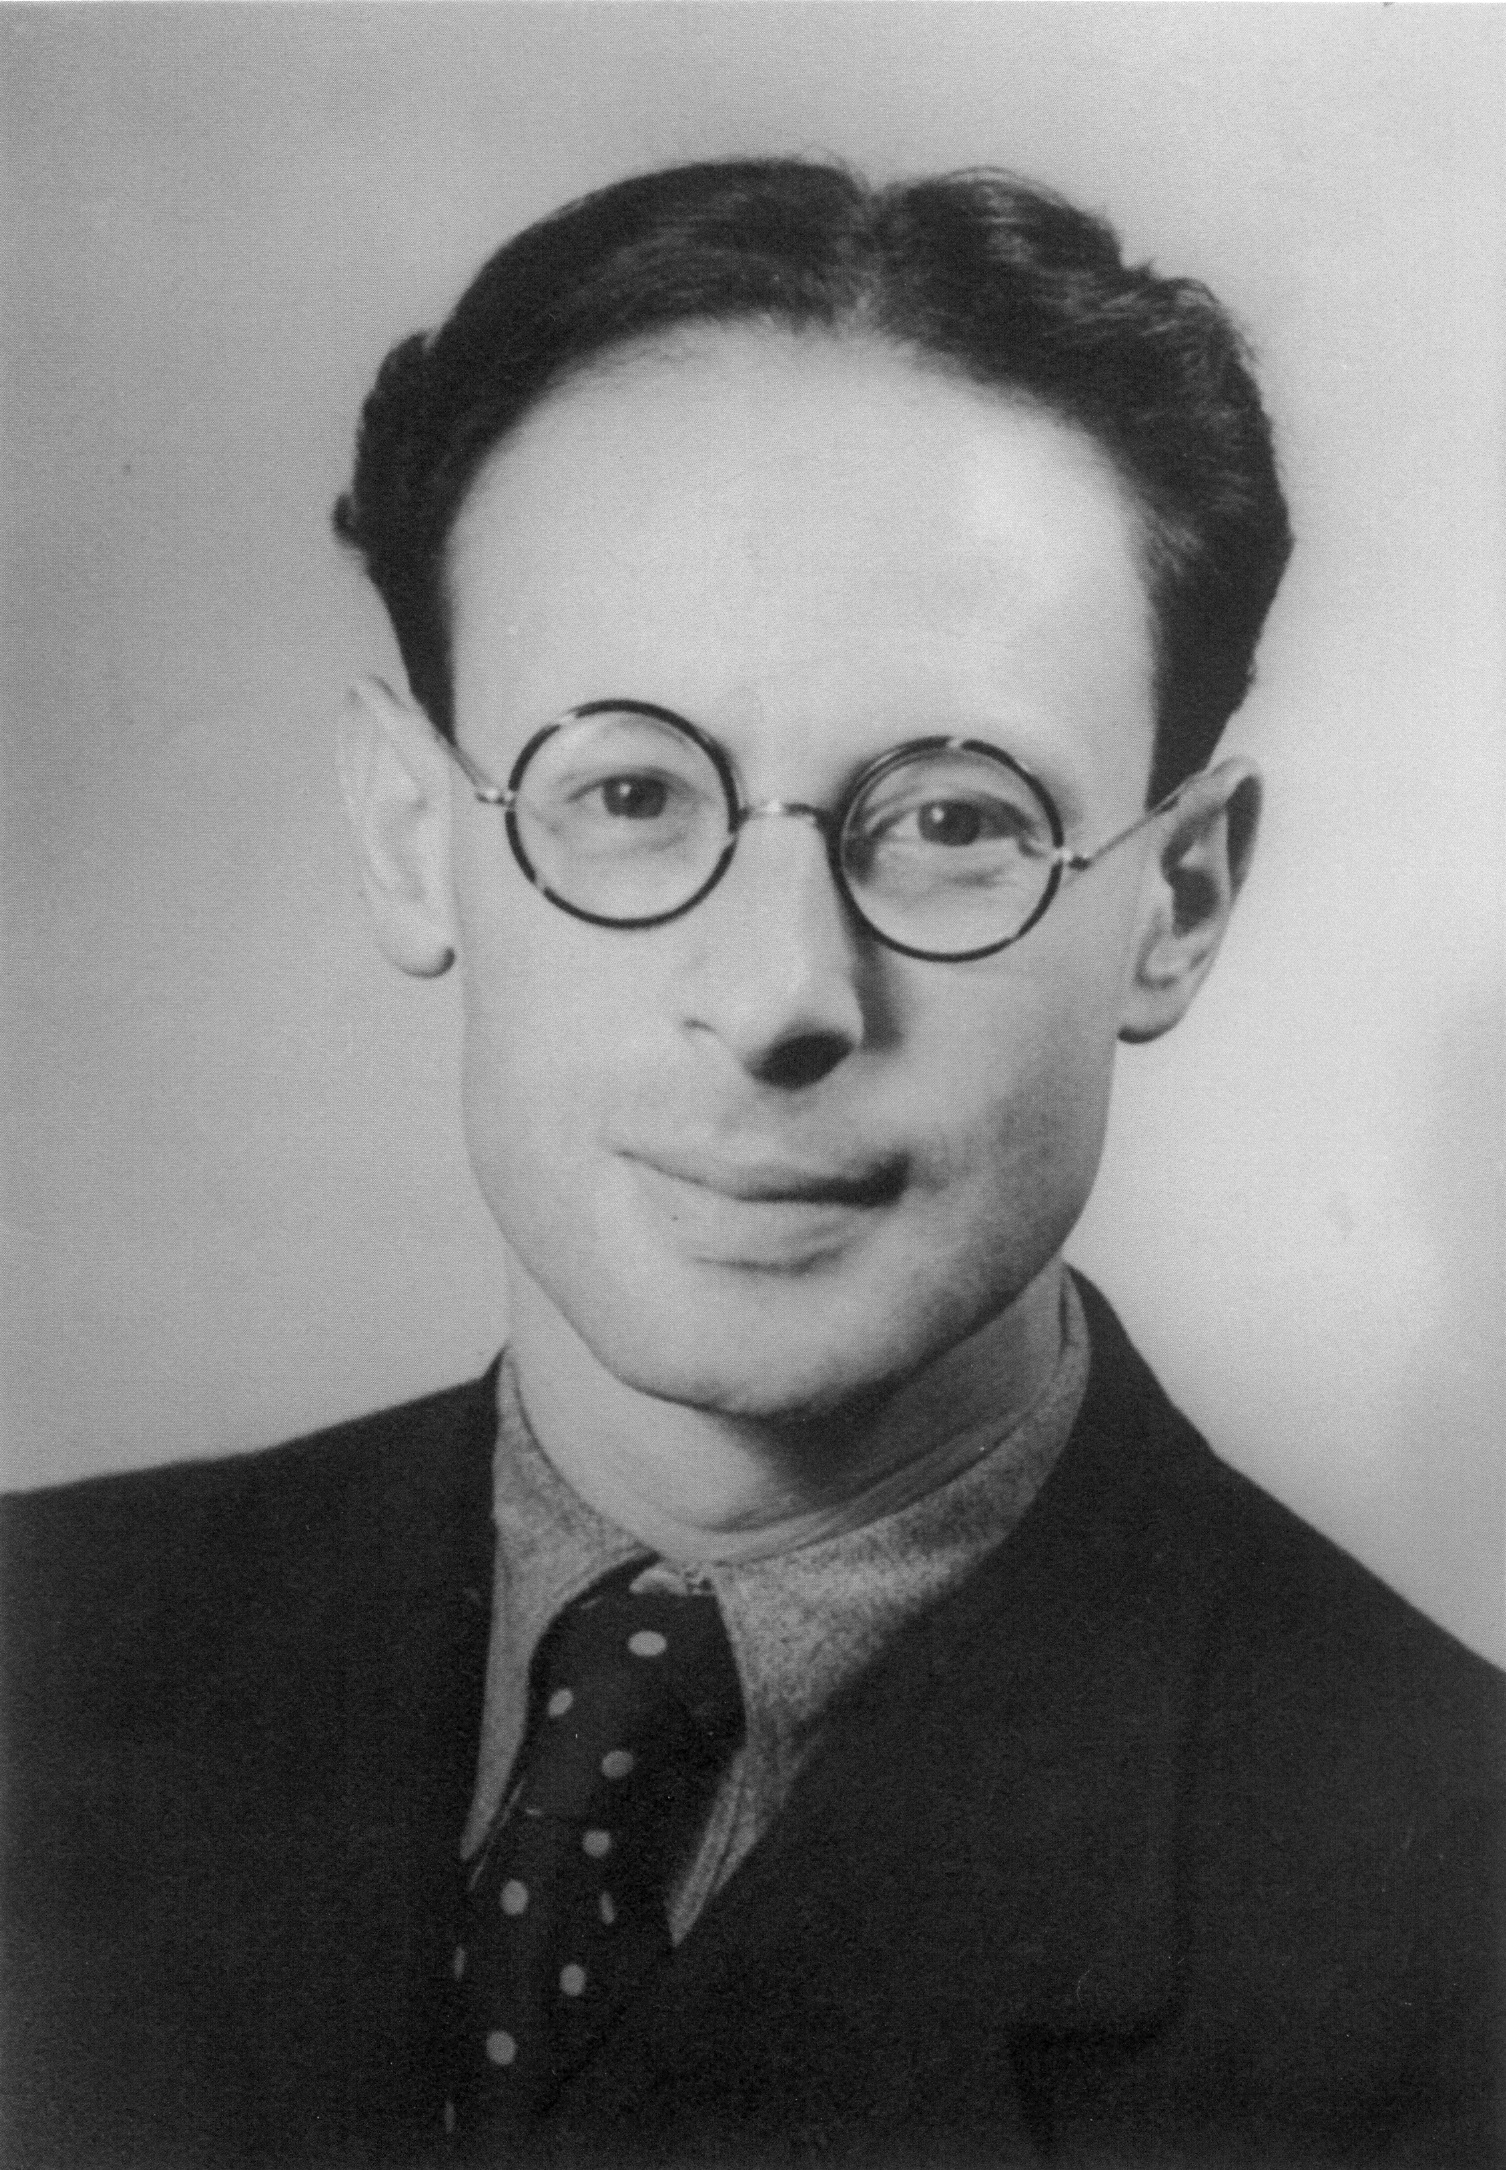
\includegraphics[scale=0.8]{images/weil}
		\caption{Andr\'e Weil.}
	\end{center}
\end{figure}

\begin{figure}
	\begin{center}
		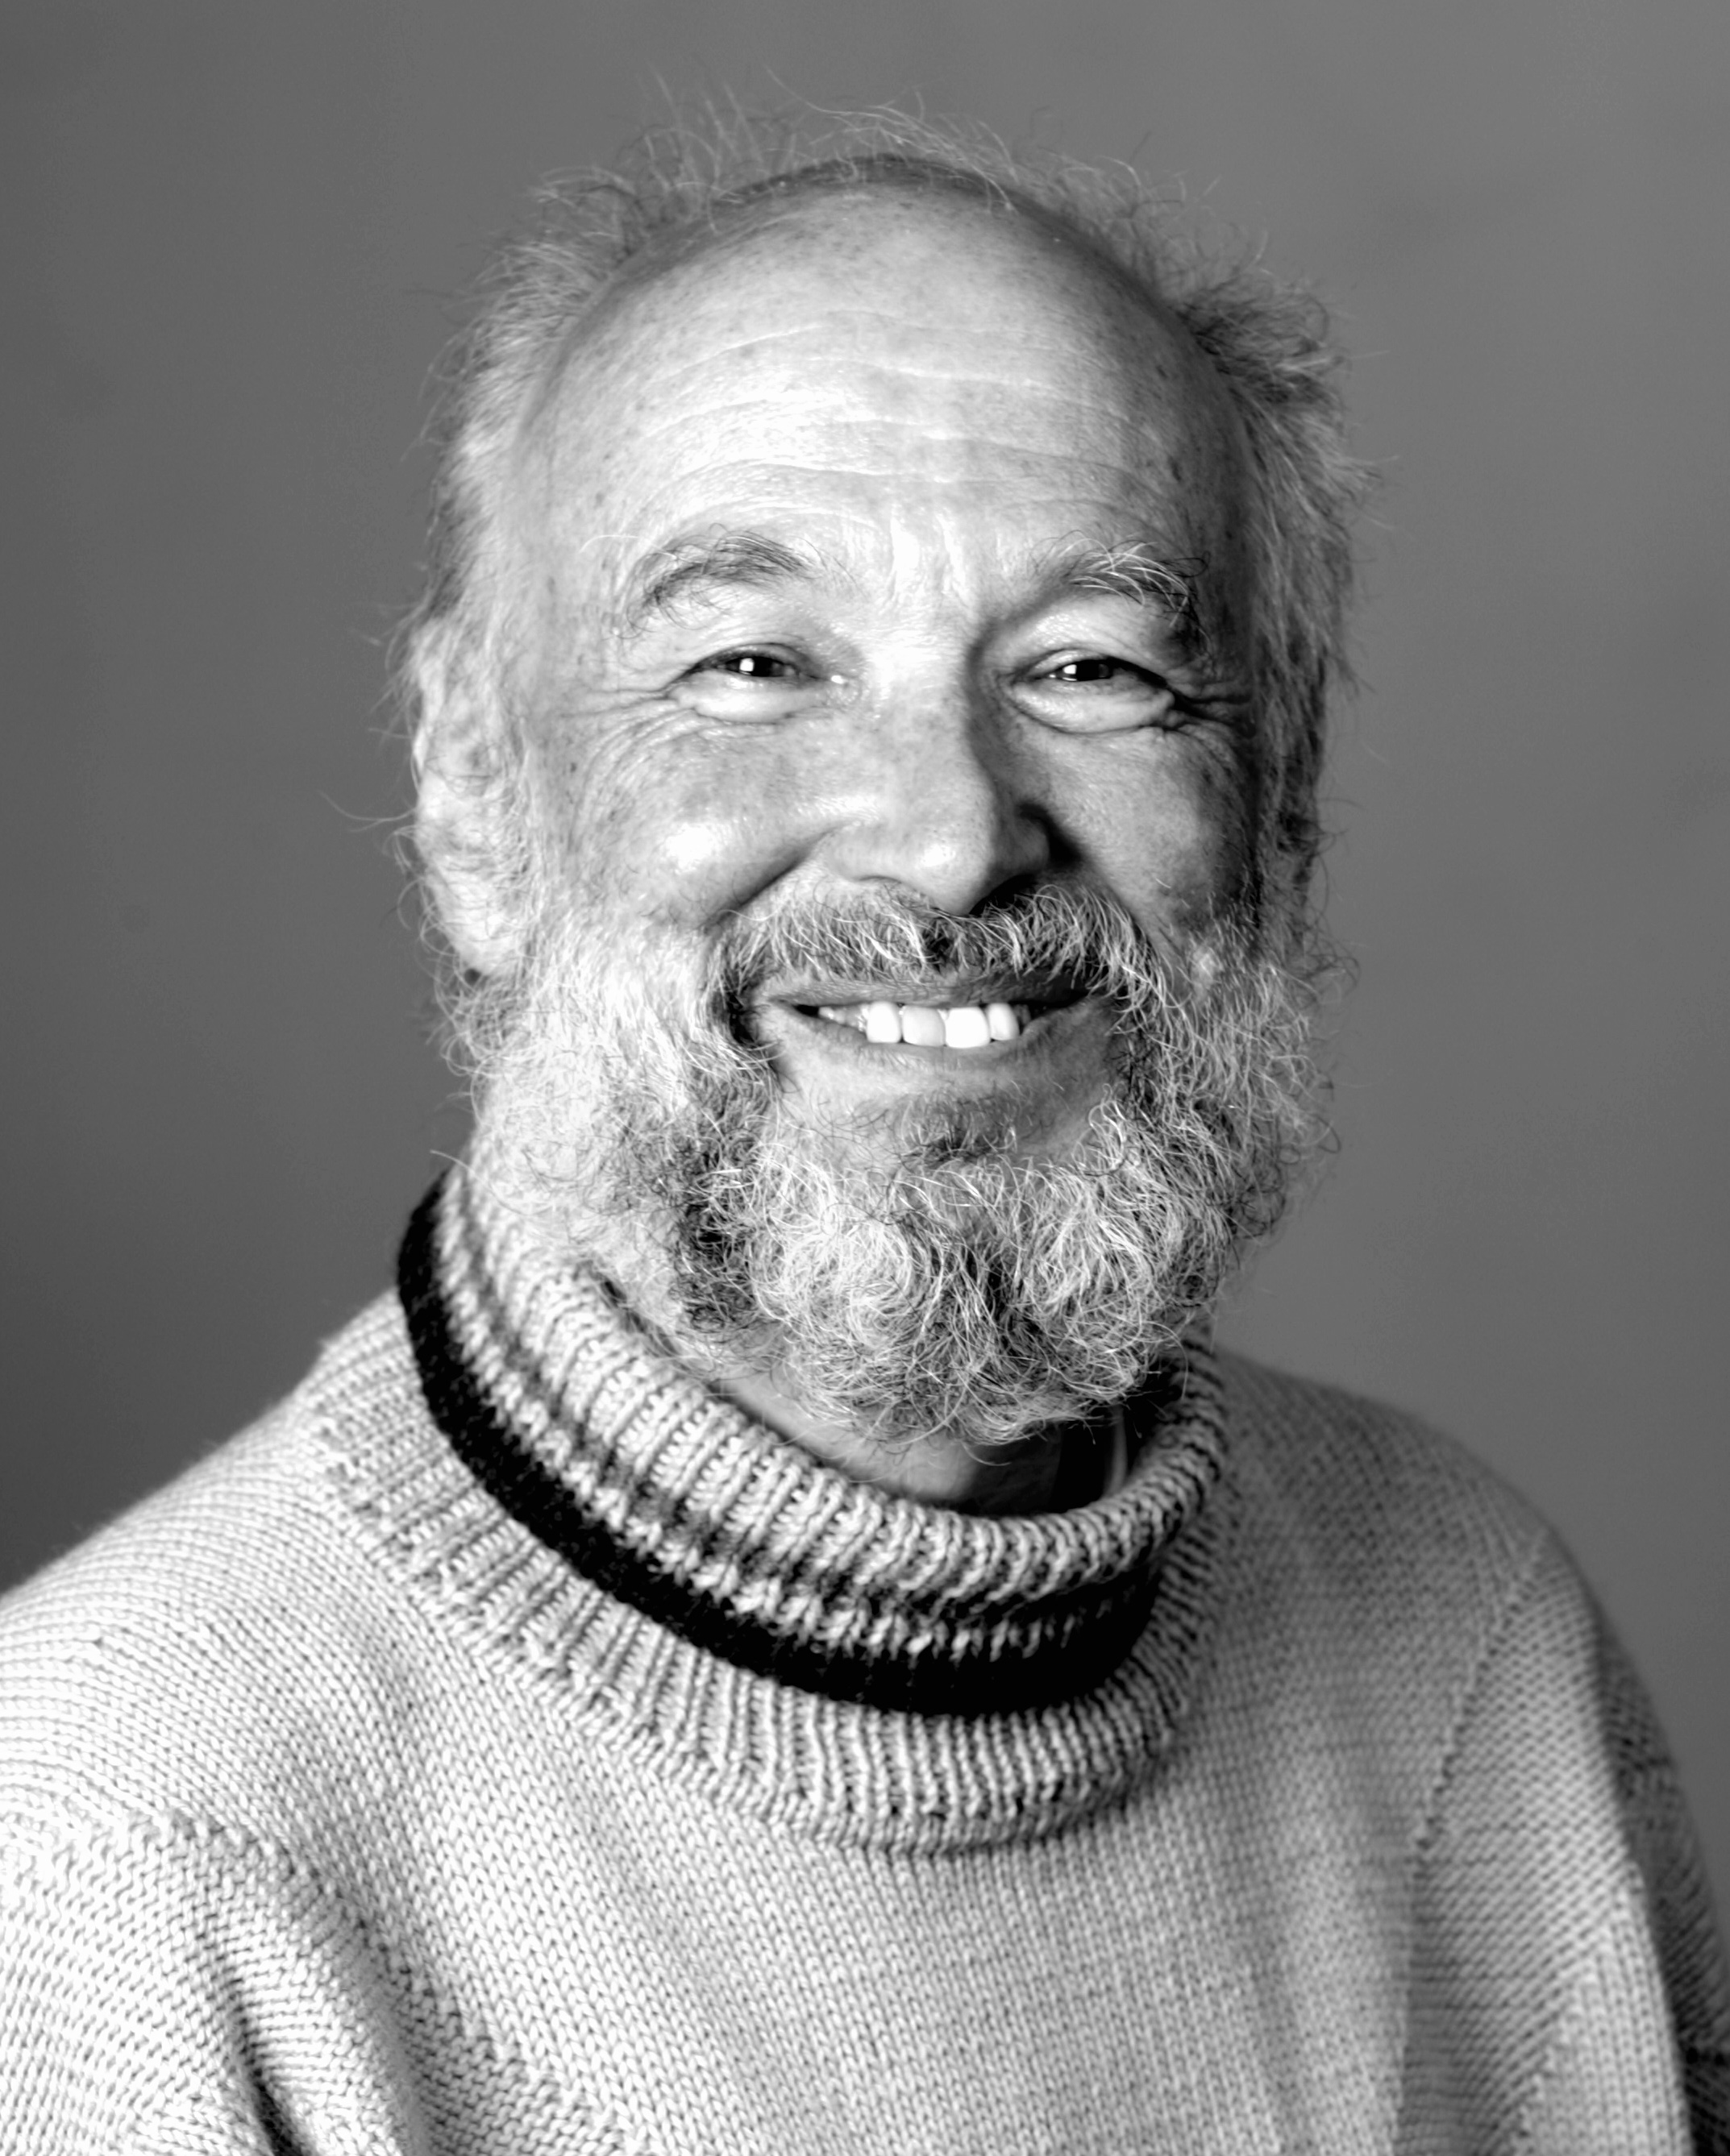
\includegraphics[scale=0.8]{images/deligne}
		\caption{Pierre Deligne.}
	\end{center}
\end{figure}

\subsection{Introduction}
\subsection{Functional equation}
\subsection{Riemann hypothesis}
\subsection{Fermat hypersurfaces}
\subsection{Lefschetz trace formula}
\subsection{\'Etale cohomology of a curve}
\subsection{\'Etale morphisms}

\section{Complex surfaces}
\subsection{Introduction}
\subsection{Minimal surfaces}
\subsection{Rational surfaces}
\subsection{Ruled surfaces}
\subsection{Kodaira: dimension $0$}
\subsection{Kodaira: dimensions $1$ and $2$}


\section{The Chow ring}
\subsection{Introduction}
\subsection{Chern classes}

\printindex
\end{document}
